\documentclass[sigconf]{acmart}

\usepackage{amsmath}
\usepackage{graphicx}
\usepackage{amsthm}
%\usepackage{amssymb}
\usepackage{thmtools}
\usepackage{color}
\usepackage{enumitem}
\usepackage{bm}
\usepackage{multirow}
\usepackage[linesnumbered, lined, boxed]{algorithm2e}

\def\calA{\mathcal{A}}
\def\calB{\mathcal{B}}
\def\calC{\mathcal{C}}
\def\calD{\mathcal{D}}
\def\calE{\mathcal{E}}
\def\calF{\mathcal{F}}
\def\calG{\mathcal{G}}
\def\calH{\mathcal{H}}
\def\calI{\mathcal{I}}
\def\calJ{\mathcal{J}}
\def\calK{\mathcal{K}}
\def\calL{\mathcal{L}}
\def\calM{\mathcal{M}}
\def\calN{\mathcal{N}}
\def\calO{\mathcal{O}}
\def\calP{\mathcal{P}}
\def\calQ{\mathcal{Q}}
\def\calR{\mathcal{R}}
\def\calS{\mathcal{S}}
\def\calT{\mathcal{T}}
\def\calU{\mathcal{U}}
\def\calV{\mathcal{V}}
\def\calW{\mathcal{W}}
\def\calX{\mathcal{X}}
\def\calY{\mathcal{Y}}
\def\calZ{\mathcal{Z}}
\def\E{\mathbb{E}}
\def\R{\mathbb{R}}
\def\Z{\mathbb{Z}}
\def\hsbm{\textnormal{HSBM}}
\def\dpcom{\textsf{DPCommunity}}
\def\dphchsbm{\textsf{DPClusterHSBM}}
\def\dphcblocks{\textsf{DPHCBlocks}}
\def\sparsecut{\textsf{SparseCut}}
\def\linkage{\textsf{Linkage}}
\newcommand{\leaves}[1]{\texttt{leaves}(#1)}

\def\dcost{\textnormal{cost}}
\def\mwcost{\textnormal{rev}}
\def\cost{\omega}
\def\mw{\textsf{MW}}
\def\DPCut{\textnormal{DPCut}}
\def\edgewgt{\textnormal{edge-wgt}}
\def\bcutcost{\textnormal{bcut-cost}}
\newcommand{\cut}[1]{\|#1\|_{\textnormal{cut}}}

%TODO Fix these
\def\citep{\cite}
\def\citet{\cite}

\newtheorem{lem}{Lemma}
\newtheorem{obs}{Observation}

%\newcommand{\Jnote}[1]{\textcolor{red}{Jacob: #1}}
%\newcommand{\Anote}[1]{\textcolor{red}{Ale: #1}}
%\newcommand{\Vnote}[1]{\textcolor{red}{Vincent: #1}}
%\newcommand{\Mnote}[1]{\textcolor{red}{Mohammed: #1}}


\SetKwInput{KwData}{Input}
\SetKwInput{KwResult}{Output}

% \newtheorem{definition}{Definition}
% \newtheorem{theorem}{Theorem}
% \newtheorem{lemma}{Lemma}
% \newtheorem{proposition}{Proposition}
% \newtheorem{corollary}{Corollary}
% \newtheorem{remark}{Remark}

% Switch conference/arXiv versions
%\newif\ifconferenceon\conferenceonfalse
\newif\ifconferenceon\conferenceontrue
\ifconferenceon
\newcommand{\conference}[1]{#1}
\newcommand{\arxiv}[1]{}
\else
\newcommand{\conference}[1]{}
\newcommand{\arxiv}[1]{#1}
\usepackage{balance}
\fi

%%
%% \BibTeX command to typeset BibTeX logo in the docs
\AtBeginDocument{%
  \providecommand\BibTeX{{%
    Bib\TeX}}}

%% Rights management information.  This information is sent to you
%% when you complete the rights form.  These commands have SAMPLE
%% values in them; it is your responsibility as an author to replace
%% the commands and values with those provided to you when you
%% complete the rights form.
% \setcopyright{acmcopyright}
% \copyrightyear{2018}
% \acmYear{2018}
% \acmDOI{XXXXXXX.XXXXXXX}

%% These commands are for a PROCEEDINGS abstract or paper.
% \acmConference[Conference acronym 'XX]{Make sure to enter the correct
%   conference title from your rights confirmation emai}{June 03--05,
%   2018}{Woodstock, NY}
% \acmPrice{15.00}
% \acmISBN{978-1-4503-XXXX-X/18/06}

\copyrightyear{2022}
\acmYear{2022}
% \setcopyright{acmcopyright}
% \setcopyright{acmlicensed}
\setcopyright{rightsretained}
\acmConference[CCS '22]{Proceedings of the 2022 ACM SIGSAC
Conference on Computer and Communications Security}{November
7--11, 2022}{Los Angeles, CA, USA}
\acmBooktitle{Proceedings of the 2022 ACM SIGSAC Conference on
Computer and Communications Security (CCS '22), November 7--11,
2022, Los Angeles, CA, USA}
\acmDOI{10.1145/3548606.3560659}
\acmISBN{978-1-4503-9450-5/22/11}
% Authors, replace the red X's with your assigned DOI string during the rightsreview eform process.
%% Your DOI link will become active when the proceedings appears in the DL.

\settopmatter{printacmref=true}

% Overwrite copyright field outside from cls file.
\usepackage{etoolbox}
\makeatletter
\patchcmd{\maketitle}{\@copyrightpermission}{
   \begin{minipage}{0.3\columnwidth}
     \href{https://creativecommons.org/licenses/by/4.0/}{\includegraphics[width=0.90\textwidth]{fig/cc_by4acm.png}}
   \end{minipage}\hfill
   \begin{minipage}{0.7\columnwidth}
     \href{https://creativecommons.org/licenses/by/4.0/}{This work is licensed under a Creative Commons Attribution International 4.0 License.}
   \end{minipage}
 
   \vspace{5pt}
}{}{}

\makeatother

%%
%% Submission ID.
%% Use this when submitting an article to a sponsored event. You'll
%% receive a unique submission ID from the organizers
%% of the event, and this ID should be used as the parameter to this command.
%%\acmSubmissionID{123-A56-BU3}

%%
%% For managing citations, it is recommended to use bibliography
%% files in BibTeX format.
%%
%% You can then either use BibTeX with the ACM-Reference-Format style,
%% or BibLaTeX with the acmnumeric or acmauthoryear sytles, that include
%% support for advanced citation of software artefact from the
%% biblatex-software package, also separately available on CTAN.
%%
%% Look at the sample-*-biblatex.tex files for templates showcasing
%% the biblatex styles.
%%

%%
%% The majority of ACM publications use numbered citations and
%% references.  The command \citestyle{authoryear} switches to the
%% "author year" style.
%%
%% If you are preparing content for an event
%% sponsored by ACM SIGGRAPH, you must use the "author year" style of
%% citations and references.
%% Uncommenting
%% the next command will enable that style.
%%\citestyle{acmauthoryear}



%%
%% end of the preamble, start of the body of the document source.
\begin{document}

%%
%% The "title" command has an optional parameter,
%% allowing the author to define a "short title" to be used in page headers.
\title{Differentially Private Triangle and 4-Cycle Counting in the Shuffle Model}

%%
%% The "author" command and its associated commands are used to define
%% the authors and their affiliations.
%% Of note is the shared affiliation of the first two authors, and the
%% "authornote" and "authornotemark" commands
%% used to denote shared contribution to the research.
\author{Jacob Imola}
\authornote{The first and second authors made equal contribution and are listed alphabetically.}
\email{jimola@eng.ucsd.edu}
\affiliation{%
  \institution{UC San Diego}
%  \streetaddress{P.O. Box 1212}
%  \city{Dublin}
%  \state{Ohio}
  \country{USA}
%  \postcode{43017-6221}
}

\author{Takao Murakami}
\authornotemark[1]
\email{takao-murakami@aist.go.jp}
\affiliation{%
  \institution{AIST}
  \country{Japan}
}

\author{Kamalika Chaudhuri}
\email{kamalika@cs.ucsd.edu}
\affiliation{%
  \institution{UC San Diego}
  \country{USA}
}

%%
%% By default, the full list of authors will be used in the page
%% headers. Often, this list is too long, and will overlap
%% other information printed in the page headers. This command allows
%% the author to define a more concise list
%% of authors' names for this purpose.
%\renewcommand{\shortauthors}{Trovato et al.}

%%
%% The abstract is a short summary of the work to be presented in the
%% article.
\begin{abstract}
Subgraph counting is fundamental for analyzing connection patterns or clustering tendencies in 
graph data. 
% a social graph. 
Recent studies have applied LDP (Local Differential Privacy) to subgraph counting to protect user privacy 
even against a data collector 
in 
% both centralized and decentralized 
social networks. 
However, existing local algorithms suffer from extremely large estimation errors or assume multi-round interaction between users and the data collector, which requires a lot of user effort and synchronization. 

In this paper, we focus on a one-round of interaction and propose accurate subgraph counting algorithms by introducing a recently studied shuffle model. 
We first propose a basic technique called \textit{wedge shuffling} to send wedge information, the main component of several subgraphs, with small noise. 
Then we apply our wedge shuffling to counting triangles and 4-cycles -- basic subgraphs for analyzing clustering tendencies -- with several additional techniques. 
% For triangles, we propose three 
% with several additional techniques, such as sending local edges to enable triangle counting, sampling independent user-pairs 
We also show upper bounds on the estimation error for each algorithm. 
We show through comprehensive experiments that our one-round shuffle algorithms significantly outperform the one-round local algorithms in terms of accuracy and achieve small estimation errors with a reasonable privacy budget, e.g., smaller than 1 in edge DP. 
%, e.g., a relative error much smaller than 1.
%with a reasonable privacy budget, e.g., smaller than 1 in edge DP. 
% our shuffle algorithms dramatically reduce the estimation error of the one-round local algorithms and achieve the relative error much smaller than 1 with a reasonable privacy budget, e.g., smaller than 1 in edge DP. 
\end{abstract}

%%
%% The code below is generated by the tool at http://dl.acm.org/ccs.cfm.
%% Please copy and paste the code instead of the example below.
%%
\begin{CCSXML}
<ccs2012>
   <concept>
       <concept_id>10002978.10002991.10002995</concept_id>
       <concept_desc>Security and privacy~Privacy-preserving protocols</concept_desc>
       <concept_significance>500</concept_significance>
       </concept>
   <concept>
       <concept_id>10002978.10003022.10003027</concept_id>
       <concept_desc>Security and privacy~Social network security and privacy</concept_desc>
       <concept_significance>500</concept_significance>
       </concept>
 </ccs2012>
\end{CCSXML}

\ccsdesc[500]{Security and privacy~Privacy-preserving protocols}
\ccsdesc[500]{Security and privacy~Social network security and privacy}

%%
%% Keywords. The author(s) should pick words that accurately describe
%% the work being presented. Separate the keywords with commas.
\keywords{differential privacy, shuffle model, subgraph counting, wedges}
%% A "teaser" image appears between the author and affiliation
%% information and the body of the document, and typically spans the
%% page.
% \begin{teaserfigure}
%   \includegraphics[width=\textwidth]{sampleteaser}
%   \caption{Seattle Mariners at Spring Training, 2010.}
%   \Description{Enjoying the baseball game from the third-base
%   seats. Ichiro Suzuki preparing to bat.}
%   \label{fig:teaser}
% \end{teaserfigure}

%%
%% This command processes the author and affiliation and title
%% information and builds the first part of the formatted document.
\maketitle

\section{Introduction}
\label{chap2-sec:intro}
Counting subgraphs (e.g., triangles, stars, cycles) is
% a fundamental task 
one of the most basic tasks 
for analyzing connection patterns
% for analyzing graph statistics
in
% a graph.
various graph data, e.g., social,
communication, and collaboration networks.
% , epidemiological networks.
% Graph statistics is important to understand the connection patterns in various graph data; e.g., social networks, collaboration networks,
% For example, a degree distribution in a social graph represents a distribution of the number of friends in the graph.
% A subgraph count (e.g.,
For example,
% a triangle count is the number of three nodes with three edges.
% A $k$-star count is the number of a node connected to $k$ other nodes.
a triangle is given by a set of three nodes with three edges, whereas a $k$-star is given by a central node connected to $k$ other nodes.
% a set of $k$ nodes connected a central node.
These subgraphs
% are important because they can be used to calculate
play a crucial role in calculating
a \textit{clustering coefficient} ($=\frac{3 \times \text{\#triangles}}{\text{\#2-stars}}$) (see Figure~\ref{chap2-fig:triangles_stars}). 
% which 
The clustering coefficient 
measures the average probability that
two friends of a user will also be a friend
% a friend's friend is also a friend
in a social graph \cite{Newman_PRL09}. 
Therefore, it is useful for measuring the effectiveness of friend suggestions. 
In addition, the clustering coefficient represents the degree to which users tend to cluster together. 
Thus, if it is large in some services/communities, we can effectively apply social recommendations \cite{Kolluri_CCS21} to the users. 
% for an example of
% the triangle and $k$-star counts and clustering coefficient).
% these subgraph counts).
% \cite{Newman_PRL09}.
% It is also known that these subgraphs are sufficient statistics for exponential random graph models
Triangles 
and $k$-stars 
% can also be used for
are also useful for 
% modeling graphs \cite{Jorgensen_SIGMOD16,Robins_SN07}.
% generating graphs based on some
constructing
graph models
\cite{Robins_SN07,Jorgensen_SIGMOD16}; 
% and other applications \cite{Imola_USENIX21}.
% (e.g., exponential random graph models \cite{Robins_SN07}, TriCycle \cite{Jorgensen_SIGMOD16}).
% Applications of triangle counting are summarized in \cite{Tsourakakis_JGAA11}. 
see also \cite{Tsourakakis_JGAA11} for other applications of triangle counting. 
However, graph data often involve sensitive data such as sensitive edges (friendships),
% that a user wants to keep secret,
% which 
and they 
can be leaked from 
% exact values of triangle counts and $k$-star counts \cite{Imola_USENIX21}.
exact numbers of triangles and $k$-stars \cite{Imola_USENIX21}.
% Therefore,
% there is a need for
% we need to develop an algorithm for
% counting
% subgraphs while strongly protecting user privacy.
% , which is the focus of this paper.


To analyze subgraphs while protecting user privacy, DP (Differential Privacy) \cite{DP} has been widely adopted as a privacy metric \cite{Ding_TKDE21,Imola_USENIX21,Karwa_PVLDB11,Sun_CCS19,Ye_ICDE20,Ye_TKDE21,Zhang_SIGMOD15}.
DP protects user privacy against adversaries with arbitrary background knowledge and is known as a gold standard for data privacy.
% Most studies on private graph analysis \cite{Chen_PoPETs20,Day_SIGMOD16,Hay_ICDM09,Karwa_PVLDB11,Kasiviswanathan_TCC13,Nissim_STOC07,Raskhodnikova_arXiv15,Song_arXiv18} assumes central DP
According to the underlying model, DP can be categorized into \textit{central (or global) DP} and \textit{LDP (Local DP)}.
Central DP assumes a scenario where
% that
a central server has personal data of all users.
% whereas LDP does not assume such trusted servers.
Although accurate analysis of subgraphs is possible under
% central DP
this model \cite{Ding_TKDE21,Karwa_PVLDB11,Zhang_SIGMOD15}, there is a risk that the entire graph is leaked from the server by illegal access or internal fraud \cite{data_breach2021,CambridgeAnalytica}.
In addition, central DP cannot be applied to  \textit{decentralized social networks} 
\cite{Diaspora,Mastodon,Minds,Paul_CN14} 
% \cite{Diaspora,Mastodon,Paul_CN14} 
% (e.g., Diaspora \cite{Diaspora}, Mastodon \cite{Mastodon}) 
% which has no central server that has the entire graph, and uses many servers each of which has personal data of users who have registered
where the entire graph is distributed across many servers. 
% nor 
We can even consider 
\textit{fully decentralized applications} where a server does not have
any original edge, 
% between users, 
% information about the original edges;
% For example,
% mobile application in which each user sends the number of her friends
e.g., a mobile app that sends a noisy degree (noisy number of friends) to the server, which then estimates a degree distribution. 
Central DP cannot be used in such applications. 

In contrast, LDP assumes a scenario where each user obfuscates her personal data (friends list in 
the case of graphs) 
% data) 
by herself and sends the obfuscated data to a possibly malicious server; i.e., it does not assume trusted servers.
Thus, it does not suffer from a data breach and can also be applied to the decentralized applications. 
% explained above.
% LDP does not assume trusted servers, hence
% can be applied to the above decentralized applications.
% In LDP, each user obfuscates her personal data (friends list in the case of graph data) by herself, and sends the obfuscated data to a (possibly malicious) server.
% Since the server does not have the original data, it does not suffer from the data breach.
LDP has been widely studied in tabular data where each row corresponds to a user's personal data (e.g., age, browser setting, location) 
\cite{Acharya_AISTATS19,Bassily_NIPS17,Erlingsson_CCS14,Kairouz_ICML16,Murakami_USENIX19,Wang_USENIX17} 
% \cite{Acharya_AISTATS19,Bassily_NIPS17,Erlingsson_CCS14,Fanti_PoPETs16,Kairouz_ICML16,Murakami_USENIX19,Qin_CCS16,Wang_USENIX17}, 
and also in graph data \cite{Imola_USENIX21,qin2017generating,Ye_ICDE20,Ye_TKDE21}.
For example, $k$-star counts can be very accurately estimated under LDP because each user can count $k$-stars of which she is a center and sends a noisy version of her $k$-star count to the server \cite{Imola_USENIX21}.

However, more complex subgraphs such as triangles are much harder to count under LDP because each user
% is not aware of
cannot see
edges between other users.
For example, in Figure~\ref{chap2-fig:triangles_stars}, user $v_1$ cannot see
% an edge between $v_2$ and $v_3$,
edges between $v_2$, $v_3$, and $v_6$ 
and therefore 
% , hence 
cannot count triangles involving $v_1$.
Thus,
% when only one-round interaction is allowed between each user and the server,
% instead of sending a noisy triangle count,
existing algorithms \cite{Imola_USENIX21,Ye_ICDE20,Ye_TKDE21}
% send noisy edges (rather than noisy triangle counts) obtained by randomized response \cite{Warner_JASA65} to a server.
obfuscate each user's edges (rather than her triangle count) by
% Warner's
RR (Randomized Response)
% randomized response
\cite{Warner_JASA65} and send noisy edges to a server.
% , which then estimates the triangle count.
% \cite{Imola_USENIX21,Ye_ICDE20,Ye_TKDE21} apply Warner's RR (Randomized Response) \cite{Warner_JASA65}, which flips 0/1 with some probability, to each edge and then estimate the triangle count.
Consequently, the server suffers from a
% very
prohibitively
large estimation error
% as shown in \cite{Imola_USENIX21} and Appendix~\ref{chap2-sec:one-round} in our paper 
(e.g., relative error $> 10^2$ in large graphs, 
as shown in Appendix~\ref{chap2-sec:one-round}) 
% (e.g., relative error $> 10^2$ in large graphs, as shown in Appendix~\ref{chap2-sec:one-round} of our paper)
because all three edges are noisy in any noisy triangle the server sees.

\begin{figure}[t]
  \centering
  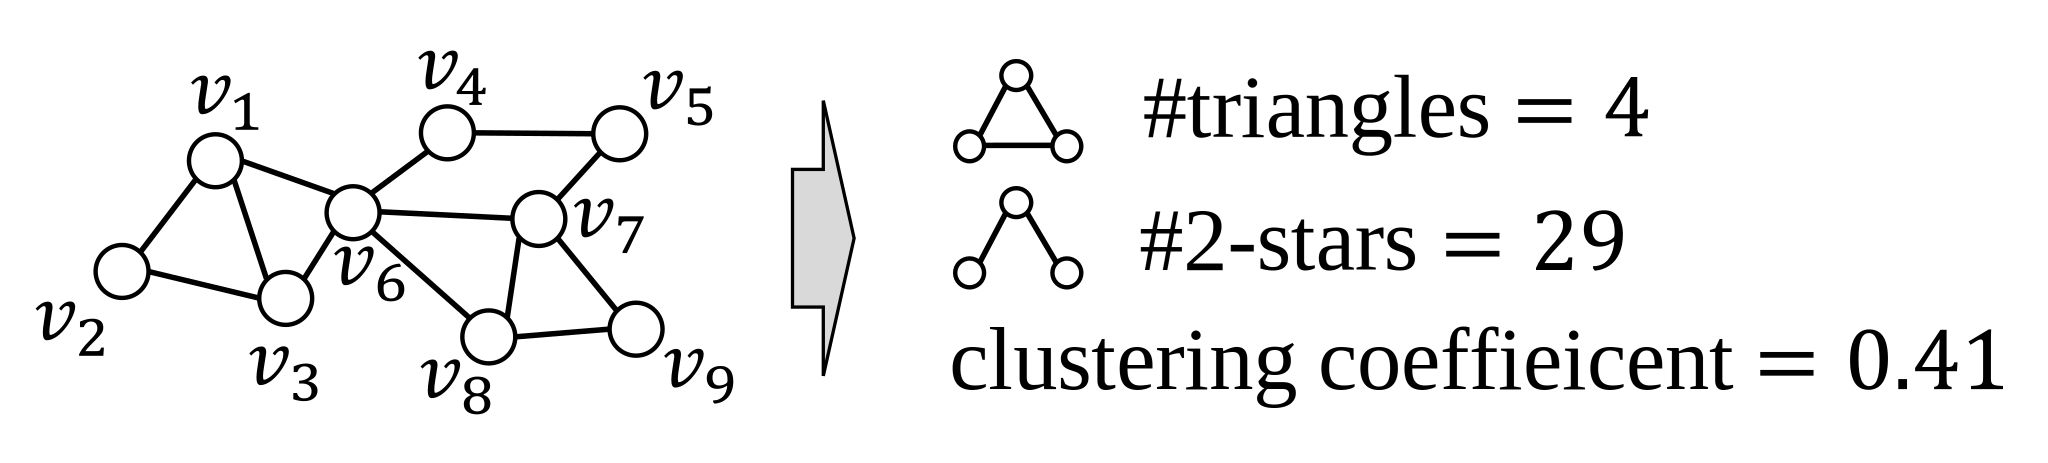
\includegraphics[width=0.85\linewidth]{fig/triangles_stars.pdf}
  
  \caption[Triangles, $2$-stars, and clustering coefficient.]{Triangles, $2$-stars, and clustering coefficient.}
  \label{chap2-fig:triangles_stars}
\end{figure}

A recent study \cite{Imola_USENIX21} shows that the estimation error in
% triangle counting under LDP
locally private triangle counting
is significantly reduced by introducing an additional round of interaction between users and the server.
Specifically, if the server publishes the noisy graph (all noisy edges) sent by users at the first round, then each user can count her noisy triangles such that \textit{only one edge} is noisy (as she knows two edges connected to her).
Thus,
% each user
the algorithm in \cite{Imola_USENIX21} sends each user's noisy triangle count (with additional noise) to the server at the second round.
Then the server can accurately estimate the triangle count. 
% between users and the server 
% The algorithm in \cite{Imola_USENIX21} 
This algorithm also requires a much smaller number of interactions 
% between users and the server 
(i.e., only two) than collaborative approaches \cite{Kairouz_FTML21,Shokri_CCS15} that generally require many interactions. 

Unfortunately, 
% this algorithm 
the algorithm in \cite{Imola_USENIX21} 
is still
% far from practical
impractical 
for a large-scale graph.
% as shown in this paper.
Specifically, the noisy graph sent by users is dense, hence extremely large for a large-scale graph, e.g.,
$500$
% $400$
Gbits for a graph of
% about $900000$ users, as in our experiments).
a million users.
The problem is that \textit{every user} needs to download such huge data; e.g., when the download speed is $20$ Mbps (which is a recommended speed in YouTube \cite{YouTube_speed}), every user needs about 7 hours to download the noisy graph.
Since the communication ability might be limited for some users, the algorithm in \cite{Imola_USENIX21} cannot be
% applied to
used for
% a large-scale graph with diverse communication environments.
applications with large and diverse users.

In summary, existing triangle algorithms under LDP suffer from either a prohibitively large estimation error or a prohibitively 
% large 
high 
communication cost.
% For the same reason, they cannot calculate the clustering coefficient
They also suffer from the same issues when calculating the clustering coefficient.

% \colorB{
% \begin{itemize}
%     \item graph statistics; e.g., degree distribution, subgraph count (e.g., 2-stars, triangles), clustering coefficient.
%     \item privacy issue, DP, central DP, LDP.
%     \item 2-star counting under LDP is easy because...
%     \item triangle counting (hence clustering coefficient) is much harder because...
%     \item Previous work \cite{Imola_USENIX21}. Communication cost is prohibitively large (e.g., 400 Gbits for \IMDB{}).
%     \item This work
% \end{itemize}}

\smallskip
\noindent{\textbf{Our Contributions.}}~~We 
% In this work, we 
propose locally private triangle counting algorithms with a small estimation error and small communication cost.
% dramatically reduce the communication cost in accurate two-rounds triangle counting under LDP
% introduce some novel algorithms
% dramatically reduce the communication cost in locally private triangle counting
% address this issue
% by introducing some novel algorithms.
% Specifically, our contributions are:
Our contributions are as follows:

\begin{itemize}
    \item We propose two-rounds triangle algorithms
% that sample edges and then select edges each user downloads.
consisting of \textit{edge sampling} after RR and \textit{selecting edges each user downloads}.
In particular, we show that a simple extension of \cite{Imola_USENIX21} with edge sampling suffers from a large estimation error for a large or dense graph where the number of 4-cycles (such as $v_1$-$v_2$-$v_3$-$v_6$-$v_1$
% and $v_4$-$v_5$-$v_7$-$v_6$-$v_4$
in Figure~\ref{chap2-fig:triangles_stars}) is large.
To address this issue, we propose some strategies for selecting edges to download to reduce the error caused by the 4-cycles, which we call the \textit{4-cycle trick}.
\item We
show that
% the above algorithms
the algorithms with the $4$-cycle trick
still suffer from a large estimation error due to
% a large global sensitivity
% a large amount of the Laplacian noise.
large Laplacian noise for each user.
% To address this, 
To significantly reduce the Laplacian noise, 
we
propose a \textit{double clipping} technique,
which clips 
a degree (the number of edges) of each user 
% the number of edges 
with LDP and then clips the number of noisy triangles. 
% to significantly reduce the Laplacian noise.
% which significantly reduces the Laplacian noise by edge clipping and noisy triangle clipping.
% consists of edge clipping and noisy triangle clipping, to significantly reduce the global sensitivity in DP \cite{DP}.
% consisting of edge clipping and noisy triangle clipping
\item We evaluate our algorithms using two real datasets.
We show that our entire algorithms with the 4-cycle trick and double clipping
% provide the best performance, and
dramatically reduce the communication cost
% when compared with
of
\cite{Imola_USENIX21}.
For example,
% when the number of users is about $900000$,
for a graph with about $900000$ users,
we reduce the download cost from $400$ Gbits ($6$ hours when $20$ Mbps) to 
% $100$ Mbits ($5$ seconds) 
$160$ Mbits ($8$ seconds) or less 
while keeping the relative error much smaller than 1.
\end{itemize}
Thus, locally private triangle counting is now much more practical. 
% Note that the number of interactions between users and a server in our algorithms (i.e, only two) is also much smaller than collaborative approaches that generally requires a number of interactions. 
In Appendix~\ref{chap2-sec:cluster}, we also show that we can estimate the clustering coefficient with a small estimation error and download cost. 
For example, our algorithms are useful for measuring the effectiveness of friend suggestions or social recommendations in decentralized 
social networks, 
% SNS, 
e.g., Diaspora \cite{Diaspora}, Mastodon \cite{Mastodon}. 
% We published
Our source code
% with C/C++
is available at 
\cite{TriangleLDP}. 
%\cite{ComTriLDP}.
% as open-source software.

All the proofs of our privacy and utility analysis 
% The proofs of all statements 
are given in \conference{the full version \cite{Imola_arXiv22}}\arxiv{Appendices~\ref{chap2-sec:proof_seq_comp_edge_LDP}, \ref{chap2-sec:proof_algorithms}, and \ref{chap2-sec:proof_double_clip}}.

\smallskip
\noindent{\textbf{Technical Novelty.}}~~Below we explain more about 
% also clarify 
the technical novelty of this paper. 
Although we focus on two-rounds local algorithms in the same way as \cite{Imola_USENIX21}, we introduce several new algorithmic ideas previously unknown in the literature. 

First, our 4-cycle trick is totally new. 
Although some studies focus on 4-cycle counting \cite{Bera_STACS17,Kallaugher_PODS19,Manjunath_ESA11,McGregor_PODS20}, this work is the first to use 4-cycles to improve communication efficiency. 
Second, selective download of parts of a centrally computed quantity is also new. 
This is not limited to graphs -- even in machine learning, 
% or federated learning, 
there are no such strategic download techniques previously, to our knowledge. 
Third, our utility analysis of our 
% two-rounds 
triangle 
algorithms (Theorem~\ref{chap2-thm:l2loss_algorithms}) is 
% also now because it 
different from \cite{Imola_USENIX21} in that ours introduces subgraphs such as 4-cycles and $k$-stars. 
This leads us to our 4-cycle trick. 
Fourth, we propose two triangle algorithms that introduce the 4-cycle trick and show that the more tricky one provides the best performance because of 
its low sensitivity in DP.
% small Laplacian noise. 

% Fourth, 
Finally, 
our double clipping is new. 
Andrew \textit{et al.} \cite{Andrew_NeurIPS21} propose an adaptive clipping technique, which applies clipping twice. 
However, they focus on federated averaging, 
% or SGD (Stochastic Gradient Descent), 
and their problem setting is different from our graph setting. 
In particular, they require a private quantile of the norm distribution. 
In contrast, we need only a much simpler estimate: a private degree. 
Here, we use the fact that the degree has a small sensitivity (sensitivity $=1$) in DP for edges. 
We also provide a new, reasonably tight bound on the probability that the noisy triangle count exceeds a clipping threshold (Theorem~\ref{chap2-thm:triangle_excess}). 
Thanks to the two differences, we obtain a significant communication improvement: two or three orders of magnitude. 

% Finally, we show an interesting finding when we combine the 4-cycle trick and double clipping. 
% Specifically, we propose two triangle algorithms that introduce the 4-cycle trick and show that the more tricky one provides the best performance because of its low sensitivity.

\section{Related Work}
\label{chap2-sec:related}
% !TEX root=main.tex
\noindent{\textbf{Triangle Counting.}}~~Triangle
% We finally note that triangle
counting has been extensively studied in a non-private setting \cite{Bera_KDD20,Bera_PODS20,Chu_KDD11,Eden_FOCS15,Seshadhri_SDM13,Suri_WWW11,Tsourakakis_KDD09,Wu_TKDE16} 
% \cite{Arifuzzaman_CIKM13,Bera_KDD20,Bera_PODS20,Chu_KDD11,Eden_FOCS15,Kolountzakis_IM12,Seshadhri_SDM13,Suri_WWW11,Tangwongsan_CIKM13,Tsourakakis_KDD09,Wu_TKDE16}
(it is almost a sub-field in itself)
because it requires high time complexity for large graphs.

Edge sampling \cite{Bera_PODS20,Eden_FOCS15,Tsourakakis_KDD09,Wu_TKDE16} is one of the most basic techniques to improve 
% the 
scalability.
Although edge sampling is simple, it is quite effective -- it is reported in \cite{Wu_TKDE16} that edge sampling outperforms other sampling techniques such as node sampling and triangle sampling.
Based on this, we adopt edge sampling after RR\footnote{We also note that a study in \cite{Nguyen_TDP16} proposes a graph publishing algorithm in the central model that independently changes 1-cells (edges) to 0-cells (no edges) with some probability and then 
changes a fixed number of 0-cells to 1-cells \textit{without replacement}. 
However, each 0-cell is \textit{not} independently sampled in this case, and consequently, 
their proof that relies on the independence of the noise to each 0-cell is incorrect. 
In contrast, our algorithms provide DP because we apply sampling after RR, i.e., post-processing.} 
with new techniques such as the 4-cycle trick and double clipping.
% to significantly improve
Our entire algorithms significantly improve the communication cost, as well as the space and time complexity, under LDP (see Sections~\ref{chap2-sub:clip_theoretical_analysis}
and \ref{chap2-sec:experiments}).
% for details).
% to significantly improve the communication cost, as well as the space and time complexity, under LDP (see Section~\ref{chap2-sub:clip_theoretical_analysis} for the performance of our entire algorithms).

\smallskip
\noindent{\textbf{DP on Graphs.}}~~For private graph analysis, DP has been widely adopted as a privacy metric.
Most of them adopt central (or global) DP
\cite{Day_SIGMOD16,Ding_TKDE21,Hay_ICDM09,Karwa_PVLDB11,Kasiviswanathan_TCC13,Raskhodnikova_arXiv15,Zhang_SIGMOD15}, 
% \cite{Chen_PoPETs20,Day_SIGMOD16,Ding_TKDE21,Hay_ICDM09,Kasiviswanathan_TCC13,Raskhodnikova_arXiv15,Song_arXiv18,Wang_TDP13,Wang_PAKDD13,Zhang_SIGMOD15}, 
which suffers from the data breach issue.
% explained above.
% in which the original graph might be leaked from the server by illegal access.

LDP on graphs has recently studied in some studies, e.g., synthetic data generation \cite{Qin_CCS17}, subgraph counting \cite{Imola_USENIX21,Sun_CCS19,Ye_ICDE20,Ye_TKDE21}.
% Sun \textit{et al.}
A study in
\cite{Sun_CCS19} proposes subgraph counting algorithms in a setting where each user
% can see all of her friends' friends.
allows her friends to see all her connections.
% However, it cannot be applied to many applications that do not allow friends to see
% Although each user can count her triangles at the first round in this setting,
However, this setting is unsuitable for
% it cannot be applied to
many applications; e.g., in Facebook, a user can easily change her setting so that
% her friend cannot see the other friends.
her friends cannot see her connections.



Thus, we consider a model where each user can see only her friends.
% , as in \cite{Sun_CCS19,Ye_ICDE20,Ye_TKDE21}.
In this model, some one-round algorithms \cite{Ye_ICDE20,Ye_TKDE21}
and two-rounds algorithms\cite{Imola_USENIX21} have been proposed.
However, they suffer from a prohibitively large estimation error or high communication cost, as explained in Section~\ref{chap2-sec:intro}.

% Recently proposed network LDP protocols \cite{Cyffers_arXiv21} consider, instead of a central server, collecting private data with user-to-user communication protocols along a graph. 
% Their results apply to sums, histograms, and SGD. 
% In our setting, we instead compute graph statistics with a central server.
% Thus, their use of graphs is orthogonal to ours. 
% The same applies to 
% another work \cite{Sabater_arXiv21} 
% that improves 
% the utility of an averaging query
% by correlating the noise of users according to a graph.
Recently proposed network LDP protocols \cite{Cyffers_arXiv21} consider, instead of a central server, collecting private data with user-to-user communication protocols along a graph. 
They focus on sums, histograms, and SGD (Stochastic Gradient Descent) and do not provide subgraph counting algorithms. 
Moreover, they focus on hiding each user's private dataset rather than hiding an edge in a graph. 
Thus, their approach cannot be applied to our task of subgraph counting under LDP for edges. 
% In our setting, we instead compute graph statistics with a central server.
% Thus, their use of graphs is orthogonal to ours. 
The same applies to 
another work \cite{Sabater_arXiv21} 
that improves 
the utility of an averaging query
by correlating the noise of users according to a graph.

\smallskip
\noindent{\textbf{LDP.}}~~RR~\cite{Kairouz_ICML16,Warner_JASA65} 
% Randomized response
and 
RAPPOR~\cite{Erlingsson_CCS14} 
% RAPPOR~\cite{Erlingsson_CCS14, Fanti_PoPETs16} 
have been widely used 
% to perform a wide range of tasks 
for tabular data 
in 
% local DP. 
LDP. 
Our work uses RR in part of our algorithm but
builds off of it significantly. One noteworthy result in this area is HR (Hadamard Response) \cite{Acharya_AISTATS19}, which is state-of-the-art for tabular data
and requires low communication. However, this result is not applied to graph
data and does not address the communication issues considered in this paper.
Specifically, applying HR to each bit in a neighbor list will result in 
% $O(n)$ communication cost 
$O(n^2)$ ($n$: \#users) download cost 
in the same way as 
the previous work \cite{Imola_USENIX21} that uses RR. 
% previous work in private, local graph
% statistics~\cite{Imola_USENIX21} does. 
Applying HR to an entire neighbor list
(which has $2^n$ possible values) will similarly result in 
% $O(\log 2^n) = O(n)$
% communication.
$O(n \log 2^n) = O(n^2)$ download cost. 

Previous work on distribution estimation~\cite{Kairouz_ICML16,Murakami_USENIX19,Wang_USENIX17} or 
% heavy hitters \cite{Bassily_NIPS17} 
heavy hitters \cite{Bassily_NIPS17} 
addresses a different problem than ours, as they assume that every user has
i.i.d. 
(independent and identically distributed) 
samples. 
In our setting, a user's neighbor list is non-i.i.d. (as one edge is shared by two users), 
% user data is an arbitrary graph, 
which does not
fit into their statistical framework.

% In work on heavy hitters in the local DP model \cite{Bassily_NIPS17,Qin_CCS16},
% each user holds a domain element and frequencies of domain elements are computed
% privately. While previous work considers user and server communication and computation
% costs as we do, their problem is not very related to our setting of graph statistics.

%\commentTM{About HR \cite{Acharya_AISTATS19}:
%Although HR is a state-of-the-art in tabular data, it is not applied to graph data and does not address the communication issue considered in this paper. For example, the communication complexity of HR (=log k) is the same as that of k-RR  (=log k), where k is category size (Table 2 in [8]). Thus,
%- if we apply HR to each bit of neighbor list, it suffers from high communication cost in the same way as our USENIX paper that uses RR.
%- if we apply HR to the whole neighbor list (n-dim vector = $2^n$ categorical data), the communication cost is high (=log $2^n$ = n).}

\section{Preliminaries}
\label{chap3-sec:preliminaries}
In this section, we describe some preliminaries for our work. 
Section~\ref{chap3-sub:notations} defines the basic notation used in this paper. 
% Sections~\ref{chap3-sub:privacy} and \ref{chap3-sub:utility} explain privacy notions and utility metrics, respectively. 
Sections~\ref{chap3-sub:privacy} and \ref{chap3-sub:shuffle} introduce DP on graphs and the shuffle model, respectively. 
Section~\ref{chap3-sub:utility} explains utility metrics. 

\subsection{Notation}
\label{chap3-sub:notations}
Let $\reals$, $\nnreals$, $\nats$, and $\nnints$ be the sets of real numbers, non-negative real numbers, natural numbers, and non-negative integers, respectively. 
% For $z\in\reals$, let $[z]$ be the set of natural numbers that do not exceed $z$. 
For $a\in\nats$, let $[a]$ be the set of natural numbers that do not exceed $a$, i.e., $[a] = \{1, 2, \ldots, a\}$. 
% Let $I_{-(i,j)} = [n]\setminus\{i,j\}$. 

We consider an undirected social graph $G=(V,E)$, where $V$ represents a set of nodes (users) and $E \subseteq V \times V$ represents a set of edges (friendships). 
Let $n\in\nats$ be the number of nodes in $V$, and $v_i \in V$ be the $i$-th node, i.e., $V=\{v_1,\ldots,v_n\}$. 
Let $I_{-(i,j)}$ be the set of indices of users other than $v_i$ and $v_j$, i.e., $I_{-(i,j)} = [n]\setminus\{i,j\}$. 
Let 
$d_i \in \nnints$ be a degree of $v_i$, 
$d_{avg} \in \nnreals$ be the average degree of $G$, and $d_{max} \in \nats$ be the maximum degree of $G$. 
In most real graphs, $d_{avg} \ll d_{max} \ll n$ holds. 
We denote a set of graphs with $n$ nodes by $\calG$. 
Let $f^\triangle: \calG \rightarrow \nnints$ and $f^\square: \calG \rightarrow \nnints$ be triangle and 4-cycle count functions, respectively. 
% Let $f^\triangle: \calG \rightarrow \nnints$ be a triangle count query. 
The triangle count function takes $G \in \calG$ as input and outputs the number $f^\triangle(G)$ of triangles in $G$, 
whereas the 4-cycle count function takes $G$ as input and outputs the number $f^\square(G)$ of 4-cycles. 
% Let $\hf^\triangle: \calG \rightarrow \reals$ be a triangle count estimator, which takes $G$ as input and outputs the estimate $\hf^\triangle(G)$ of triangles. 

Let $\bmA=(a_{i,j}) \in \{0,1\}^{n \times n}$ be 
%a symmetric 
an adjacency matrix corresponding to $G$. 
% $a_{i,j} = 1$ if and only if $(v_i,v_j) \in E$. 
If $(v_i,v_j) \in E$, then $a_{i,j} = 1$; otherwise, $a_{i,j} = 0$. 
We call $a_{i,j}$ an \textit{edge indicator}. 
Let $\bma_i \in \{0,1\}^n$ be a neighbor list of user $v_i$, i.e., the $i$-th row of $\bmA$. 
\arxiv{Table~\ref{chap3-tab:notations} shows the basic notation in this paper.} 
% We summarize the basic notation in Table~\ref{chap3-tab:notations} of Appendix~\ref{chap3-sec:notation_table}.

\arxiv{\begin{table}[t]
\caption{Basic notation in this paper.}

\centering
\hbox to\hsize{\hfil
\begin{tabular}{l|l}
\hline
Symbol		&	Description\\
\hline
% $I_{-(i,j)}$    &   Set of user indices other than $i$ and $j$ ($[n]\setminus\{i,j\}$).\\
$G=(V,E)$   &	    Undirected social graph.\\
$n$         &	    Number of nodes (users).\\
$v_i$       &       $i$-th user in $V$, i.e., $V=\{v_1,\ldots,v_n\}$.\\
% $I_{-(i,j)}$    &   Set of user indices other than $i$ and $j$ ($[n]\setminus\{i,j\}$).\\
$I_{-(i,j)}$    &   $=[n]\setminus\{i,j\}$.\\
$d_i$   &       Degree of $v_i$.\\
$d_{avg}$   &       Average degree in $G$.\\
$d_{max}$   &       Maximum degree in $G$.\\
$\calG$     &       Set of possible graphs with $n$ nodes.\\
$f^\triangle(G)$   &  Triangle count in graph $G$.\\
$f^\square(G)$   &  4-cycle count in graph $G$.\\
% $\hf^\triangle(G)$   &  Estimate of the triangle count in graph $G$.\\
$\bmA=(a_{i,j})$	    &		Adjacency matrix.\\
% $a_{i,j}$	&		Edge indicator between $v_i$ and $v_j$.\\
$\bma_i$	&		Neighbor list of $v_i$, i.e., the $i$-th row of $\bmA$.\\
% $\calR_i$     &       Local randomizer of $v_i$.\\
\hline
\end{tabular}
\hfil}
\label{chap3-tab:notations}
\end{table}}

% \subsection{Privacy Notions}
\subsection{Differential Privacy}
\label{chap3-sub:privacy}
% \smallskip
% \noindent{\textbf{$(\epsilon,\delta)$-DP.}}~~
\noindent{\textbf{DP and LDP.}}~~We use differential privacy, and more specifically $(\epsilon,\delta)$-DP \cite{DP}, as a privacy metric: 

\begin{definition} [$(\epsilon,\delta)$-DP \cite{DP}] \label{chap3-def:DP} 
Let $n \in \nats$ be the number of users. 
Let $\epsilon \in \nnreals$ and $\delta \in [0,1]$. 
Let $\calX$ be the set of input data for each user. 
%Let 
%$\calM: \calX^n \rightarrow \calS$ 
% $\calM$ 
%be a randomized algorithm. 
A randomized algorithm $\calM$ with domain $\calX^n$ 
provides \emph{$(\epsilon,\delta)$-DP} if for any neighboring databases $D,D' \in \calX^n$ that differ in a single user's data and any 
%$s \in \calS$, 
$S \subseteq \mathrm{Range}(\calM)$, 
\begin{align*}
\Pr[\calM(D) \in S] \leq e^\epsilon \Pr[\calM(D') \in S] + \delta.
%\label{chap3-eq:DP}
\end{align*}
% We say $\calM$ provides \emph{$\epsilon$-DP} if it provides \emph{$(\epsilon,0)$-DP}.
\end{definition}
$(\epsilon,\delta)$-DP guarantees that two neighboring datasets $D$ and $D'$ are almost equally likely when $\epsilon$ and $\delta$ are close to $0$. 
The parameter $\epsilon$ is called the privacy budget. 
It is well known that $\epsilon \leq 1$ is acceptable and $\epsilon \geq 5$ is unsuitable in many practical scenarios \cite{DP_Li}. 
In addition, the parameter $\delta$ needs to be much smaller than $\frac{1}{n}$ \cite{Barber_arXiv14,DP}. 

% Note that $(\epsilon,\delta)$-LDP (Local DP) is a special case of $(\epsilon,\delta)$-DP in Definition~\ref{chap3-def:DP} where $n=1$. 
% Note that $(\epsilon,\delta)$-DP in Definition~\ref{chap3-def:DP} covers the local model where each user obfuscates her personal data by herself. 
% Specifically, we can apply $(\epsilon,\delta)$-DP to the local model by setting $n=1$. 
% In this case, a randomized algorithm $\calM$ is called a \textit{local randomizer}. 
LDP \cite{Kasiviswanathan_FOCS08} is a special case of DP where $n=1$. 
In this case, a randomized algorithm is called a \textit{local randomizer}. 
We denote the local randomizer by $\calR$ to distinguish it from the randomized algorithm $\calM$ in the central model. 
Formally, LDP is defined as follows: 
\begin{definition} [$\epsilon$-LDP \cite{Kasiviswanathan_FOCS08}] \label{chap3-def:LDP} 
Let $\epsilon \in \nnreals$. 
Let $\calX$ be the set of input data for each user. 
A local randomizer $\calR$ with domain $\calX$ 
provides \emph{$\epsilon$-LDP} if for any $x,x' \in \calX$ and any $S \subseteq \mathrm{Range}(\calR)$, 
\begin{align}
\Pr[\calR(x) \in S] \leq e^\epsilon \Pr[\calR(x') \in S].
\label{chap3-eq:LDP}
\end{align}
\end{definition}

% \begin{table}[t]
% \caption{Basic notations in this paper.}
% 
% \centering
% \hbox to\hsize{\hfil
% \begin{tabular}{l|l}
% \hline
% Symbol		&	Description\\
% \hline
% % $I_{-(i,j)}$    &   Set of user indices other than $i$ and $j$ ($[n]\setminus\{i,j\}$).\\
% $G=(V,E)$   &	    Undirected social graph.\\
% $n$         &	    Number of nodes (users).\\
% $v_i$       &       $i$-th user in $V$, i.e., $V=\{v_1,\ldots,v_n\}$.\\
% % $I_{-(i,j)}$    &   Set of user indices other than $i$ and $j$ ($[n]\setminus\{i,j\}$).\\
% $I_{-(i,j)}$    &   $=[n]\setminus\{i,j\}$.\\
% $d_{avg}$   &       Average degree in $G$.\\
% $d_{max}$   &       Maximum degree in $G$.\\
% $\calG$     &       Set of possible graphs with $n$ nodes.\\
% $f^\triangle(G)$   &  Triangle count in graph $G$.\\
% $f^\square(G)$   &  4-cycle count in graph $G$.\\
% % $\hf^\triangle(G)$   &  Estimate of the triangle count in graph $G$.\\
% $\bmA=(a_{i,j})$	    &		Adjacency matrix.\\
% % $a_{i,j}$	&		Edge indicator between $v_i$ and $v_j$.\\
% $\bma_i$	&		Neighbor list of $v_i$, i.e., the $i$-th row of $\bmA$.\\
% % $\calR_i$     &       Local randomizer of $v_i$.\\
% \hline
% \end{tabular}
% \hfil}
% \label{chap3-tab:notations}
% \end{table}

\smallskip
\noindent{\textbf{Randomized Response.}}~~We use Warner's RR (Randomized Response) \cite{Warner_JASA65} to provide 
% $\epsilon$-
LDP. 
% in the local model. 
Given $\epsilon \in \nnreals$, Warner's RR $\calR_{\epsilon}^W: \{0,1\} \rightarrow \{0,1\}$ maps $x \in \{0,1\}$ to $y \in \{0,1\}$ with the probability: 
\begin{align*}
    \Pr[\calR_{\epsilon}^W(x) = y] = 
    \begin{cases}
    \frac{e^\epsilon}{e^\epsilon + 1}   &   \text{(if $x=y$)} \\
    \frac{1}{e^\epsilon + 1}   &   \text{(otherwise)}.
    \end{cases}
\end{align*}
$\calR_{\epsilon}^W$ 
% $\epsilon$-RR 
provides $\epsilon$-LDP in Definition~\ref{chap3-def:LDP}, where $\calX = \{0,1\}$. 
We refer to Warner's RR $\calR_{\epsilon}^W$ with parameter $\epsilon$ as \textit{$\epsilon$-RR}. 
% $\epsilon$-DP in Definition~\ref{chap3-def:DP}, where $\calX = \{0,1\}$ and $n=1$. 
% We call $\calR_{\epsilon}^W$ the $\epsilon$-RR.

% \commentTM{Below, we could include the following:
% \begin{itemize}
% \item Motivation of introducing $(\epsilon, \delta)$-element DP, e.g., to be consistent with existing edge LDP \cite{qin2017generating} that considers the difference of one element.
% \item $(\epsilon, \delta)$-element DP $\rightarrow$ $(2\epsilon, 2\delta)$-edge DP.
% \end{itemize}}

\smallskip
\noindent{\textbf{DP on Graphs.}}~~For graphs, we can consider two types of DP: 
% When we apply DP to graphs, we can consider two types of definitions: 
\textit{edge DP} and \textit{node DP} \cite{Hay_ICDM09,Raskhodnikova_Encyclopedia16}. 
Edge DP hides the existence of one edge, whereas node DP hides the existence of one node along with its adjacent edges. 
% Node DP is much harder to attain
In this paper, we focus on edge DP because existing one-round local triangle counting algorithms \cite{Imola_USENIX21,Imola_USENIX22,Ye_ICDE20,Ye_TKDE21} use edge DP. 
%one-round local triangle (or 4-cycle) counting requires too large $\epsilon$ even in edge DP, as shown in our experiments. 
In other words, we are interested in 
% how much $\epsilon$ in edge DP is reduced (or 
how much the estimation error is reduced at the same value of $\epsilon$ in edge DP by shuffling. 
% We also provide a new lower bound on the estimation error to illustrate the limitations of edge DP in the local model. 
Although node DP is much stronger than edge DP, it is much harder to attain and often results in a much larger $\epsilon$ \cite{Chen_SIGMOD13,Sajadmanesh_arXiv22}. 
Thus, we leave an algorithm for shuffle node DP with small $\epsilon$ (e.g., $\epsilon \leq 1$) for future work. 
Another interesting avenue of future work is establishing a lower bound on the estimation error for node DP. 
%on the estimation error to illustrate the limitations of shuffle node DP. 
% an interesting avenue of future work would be an algorithm for shuffle node DP with small $\epsilon$ (e.g., $\epsilon \leq 1$) or a lower bound on the estimation error to illustrate the limitations of shuffle node DP.

Edge DP assumes that anyone (except for user $v_i$) can be an adversary who infers edges of user $v_i$ and that the adversary can obtain all edges except for edges of $v_i$ as background knowledge. 
% When we apply edge DP to the shuffle model, we note 
Note that the central and local models have different definitions of neighboring data in edge DP. 
Specifically, edge DP in the central model \cite{Raskhodnikova_Encyclopedia16} considers two graphs that differ in one edge. 
In contrast, edge LDP 
% (Local DP) 
\cite{qin2017generating} considers two neighbor lists that differ in one bit: 
%element (bit). 

\begin{definition} [$(\epsilon,\delta)$-edge DP \cite{Raskhodnikova_Encyclopedia16}] \label{chap3-def:edge_DP} 
Let $n \in \nats$, $\epsilon \in \nnreals$, and $\delta \in [0,1]$. 
A randomized algorithm $\calM$ with domain $\calG$ provides \emph{$(\epsilon, \delta)$-edge DP} 
if for any two neighboring graphs $G, G' \in \calG$ that differ in \textbf{one edge} and any $S \subseteq \mathrm{Range}(\calM)$, 
\begin{align*}
\Pr[\calM(G) \in S] \leq e^\epsilon \Pr[\calM(G') \in S] + \delta.
%\label{chap3-eq:edge_DP}
\end{align*}
% We say $\calM$ provides \emph{$\epsilon$-edge DP} if it provides \emph{$(\epsilon,0)$-edge DP}.
\end{definition}

\begin{definition} [$\epsilon$-edge LDP~\cite{qin2017generating}] \label{chap3-def:edge_LDP} 
Let $\epsilon \in \nnreals$. 
A local randomizer $\calR$ with domain $\{0,1\}$ provides \emph{$\epsilon$-edge LDP} if for any two neighbor lists $\bma_i, \bma'_i \in \{0,1\}^n$ that differ in \textbf{one bit} and any $S \subseteq \mathrm{Range}(\calR)$, 
\begin{align*}
\Pr[\calR(\bma_i) \in S] \leq e^\epsilon \Pr[\calR(\bma'_i) \in S].
%\label{chap3-eq:edge_LDP}
\end{align*}
\end{definition}

% To deal with these differences, 
As with edge LDP,  
we define \textit{element DP}, which considers two adjacency matrices that differ in one bit, in the central model:

\begin{definition} [$(\epsilon,\delta)$-element DP] \label{chap3-def:element_DP} 
Let $n \in \nats$, $\epsilon \in \nnreals$, and $\delta \in [0,1]$. 
A randomized algorithm $\calM$ with domain $\calG$ provides \emph{$(\epsilon, \delta)$-element DP} 
if for any two neighboring graphs $G, G' \in \calG$ that differ in \textbf{one bit} in the corresponding adjacency matrices $\bmA, \bmA' \in \{0,1\}^{n \times n}$
and any $S \subseteq \mathrm{Range}(\calM)$, 
\begin{align*}
\Pr[\calM(G) \in S] \leq e^\epsilon \Pr[\calM(G') \in S] + \delta.
%\label{chap3-eq:element_DP}
\end{align*}
% We say $\calM$ provides \emph{$\epsilon$-element DP} if it provides \emph{$(\epsilon,0)$-element DP}.
\end{definition}

% Element DP considers two graphs that differ in one element, as with edge LDP. 
% In contrast, edge DP \cite{Raskhodnikova_Encyclopedia16} considers two graphs that differ in one edge: 

% \begin{definition} [$(\epsilon,\delta)$-edge DP \cite{Raskhodnikova_Encyclopedia16}] \label{chap3-def:edge_DP} 
% Let $n \in \nats$, $\epsilon \in \nnreals$, and $\delta \in [0,1]$. 
% A randomized algorithm $\calM$ with domain $\calG$ provides \emph{$(\epsilon, \delta)$-edge DP} 
% if for any two neighboring graphs $G, G' \in \calG$ that differ in \textbf{one edge} and any $S \subseteq \mathrm{Range}(\calM)$, 
% \begin{align}
% \Pr[\calM(G) \in S] \leq e^\epsilon \Pr[\calM(G') \in S] + \delta.
% \label{chap3-eq:edge_DP}
% \end{align}
% % We say $\calM$ provides \emph{$\epsilon$-edge DP} if it provides \emph{$(\epsilon,0)$-edge DP}.
% \end{definition}

Although element DP and edge DP have different definitions of neighboring data, they are closely related to each other:

\begin{proposition}\label{chap3-prop:element_edge_DP}
If a randomized algorithm $\calM$ provides $(\epsilon, \delta)$-element DP, it also provides $(2\epsilon, 2\delta)$-edge DP. 
\end{proposition}
\begin{proof}
Adding or removing one edge affects two bits in an adjacency matrix. 
Thus, by group privacy \cite{DP}, any 
% randomized 
$(\epsilon, \delta)$-element DP 
algorithm $\calM$ 
% providing $(\epsilon, \delta)$-element DP 
provides $(2\epsilon, 2\delta)$-edge DP. 
\end{proof}
Similarly, if 
% each user applies a local randomizer $\calR$ providing 
a randomized algorithm $\calM$ in the central model 
%consists of $n$ local randomizers $\calR$
applies a local randomizer $\calR$ providing $\epsilon$-edge LDP to each neighbor list $\bma_i$ ($1 \leq i \leq n$), it provides $2\epsilon$-edge DP \cite{Imola_USENIX21}. 

In this work, we use the shuffling technique to provide $(\epsilon, \delta)$-element DP and then Proposition~\ref{chap3-prop:element_edge_DP} to provide $(2\epsilon, 2\delta)$-edge DP. 
We also compare our shuffle algorithms providing $(\epsilon, \delta)$-element DP and $(2\epsilon, 2\delta)$-edge DP with local algorithms providing $\epsilon$-edge LDP and $2\epsilon$-edge DP to see how much the estimation error is reduced by introducing the shuffle model and a very small $\delta$ ($\ll \frac{1}{n}$). 

% \subsection{Shuffle Privacy Model}
\subsection{Shuffle Model}
\label{chap3-sub:shuffle}
We consider the following shuffle model. 
% for graphs. 
% Each user $v_i \in V$ obfuscates input data calculated from her neighbor list $\bma_i$ 
Each user $v_i \in V$ obfuscates her personal data 
using a local randomizer $\calR$ providing $\epsilon_L$-LDP for $\epsilon_L \in \nnreals$. 
Note that $\calR$ is common to all users. 
User $v_i$ encrypts the obfuscated data and sends it to a shuffler. 
Then, the shuffler randomly shuffles the encrypted data and sends the results to a data collector. 
Finally, the data collector decrypts them. 
The common assumption in the shuffle model is that the shuffler and the data collector do not collude with each other. 
Under this assumption, the shuffler cannot access the obfuscated data, and the data collector cannot link the obfuscated data to the users. 
Hereinafter, we omit the encryption/decryption process because it is clear from the context. 
%irrelevant to our techniques. 
% Then, the shuffler does not know the obfuscated data, and the data collector does not know which obfuscated data corresponds to which user. 

% We use the following privacy amplification result provided by Feldman \textit{et al.} \cite{Feldman_FOCS21}:
We use the privacy amplification result by Feldman \textit{et al.} \cite{Feldman_FOCS21}:
\begin{theorem} [Privacy amplification by shuffling \cite{Feldman_FOCS21}] \label{chap3-thm:shuffle}
Let $n \in \nats$ and $\epsilon_L \in \nnreals$. 
Let $\calX$ be the set of input data for each user. 
Let $x_i \in \calX$ be input data of the $i$-th user, and 
% Let 
$x_{1:n} = (x_1, \cdots, x_n) \in \calX^n$. 
Let $\calR: \calX \rightarrow \calY$ be a local randomizer providing $\epsilon_L$-LDP. 
Let $\calM_S: \calX^n \rightarrow \calY^n$ be an algorithm that given a dataset $x_{1:n}$, computes $y_i = \calR(x_i)$ for $i \in [n]$, samples a uniform random permutation $\pi$ over $[n]$, and outputs $y_{\pi(1)}, \ldots, y_{\pi(n)}$. 
Then for any $\delta \in [0,1]$ such that $\epsilon_L \leq \log (\frac{n}{16 \log (2/\delta)})$, $\calM_S$ provides $(\epsilon, \delta)$-DP, where
\begin{align}
\epsilon = f(n, \epsilon_L, \delta)
\label{chap3-eq:shuffle_epsilon_f}
\end{align}
and 
\begin{align}
f(n, \epsilon_L, \delta) = \log \left( 1 + \frac{e^{\epsilon_L}-1}{e^{\epsilon_L}+1} \left( \frac{8\sqrt{e^{\epsilon_L} \log(4/\delta)}}{\sqrt{n}} + \frac{8 e^{\epsilon_L}}{n} \right) \right).
\label{chap3-eq:shuffle_epsilon}
\end{align}
\end{theorem}
% \begin{figure}[t]
%   \centering
%   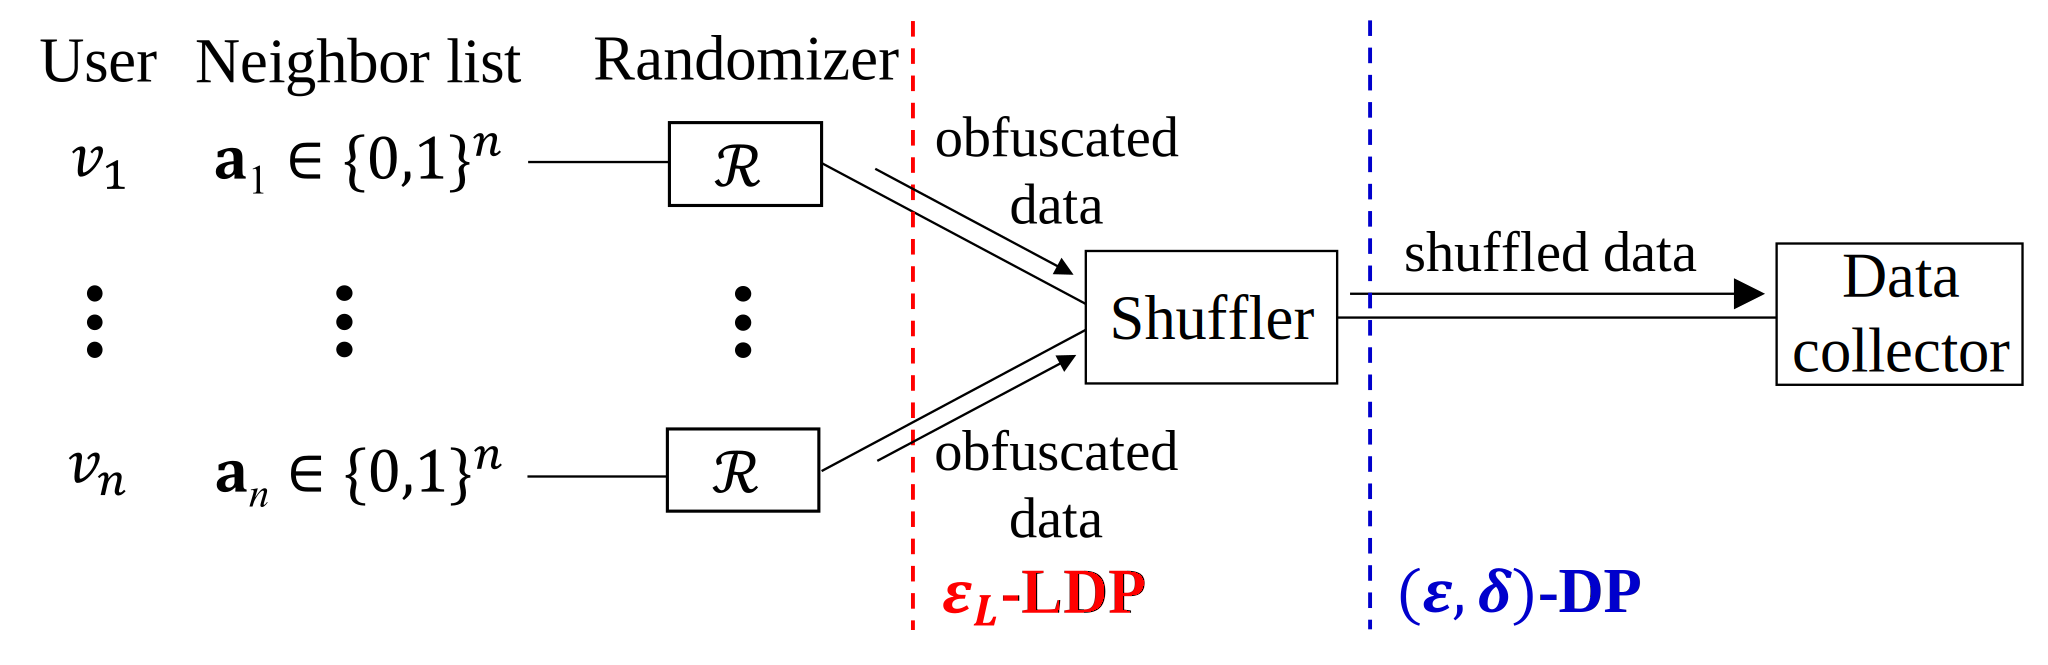
\includegraphics[width=0.99\linewidth]{fig/shuffle.pdf}
%   
%   \caption{Shuffle model. 
%   User $v_i$ obfuscates input data $x_i$ 
%   % calculated from her neighbor list $\bma_i$ 
%   and sends the obfuscated data $y_i$ to the shuffler. 
%   The shuffler sends shuffled data $y_{\pi(1)}, \ldots, y_{\pi(n)}$ to the data collector.
%   }
%   \label{chap3-fig:shuffle_model}
% \end{figure}
% Figure~\ref{chap3-fig:shuffle_model} shows the shuffle model assumed in this paper. 
Thanks to the shuffling, the shuffled data $y_{\pi(1)}, \ldots, y_{\pi(n)}$ available to the data collector provides $(\epsilon, \delta)$-DP, where $\epsilon \ll \epsilon_L$. 

Feldman \textit{et al.} \cite{Feldman_FOCS21} also propose an efficient method to numerically compute a tighter upper bound than the closed-form upper bound in Theorem~\ref{chap3-thm:shuffle}. 
We use both the closed-form and numerical upper bounds in our experiments. 
Specifically, we use the numerical upper bounds in Section~\ref{chap3-sec:experiments} and compare the numerical bound with the closed-form bound in 
\conference{the full version \cite{Imola_CCSFull22}}\arxiv{Appendix~\ref{chap3-sec:numerical_closed}}. 

Assume that $\epsilon$ and $\delta$ in (\ref{chap3-eq:shuffle_epsilon}) are constants. 
Then, by solving for $\epsilon_L$ and changing to big $O$ notation, we obtain  $\epsilon_L = \log(n) + O(1)$. 
This is consistent with the upper bound $\epsilon = O(e^{\epsilon_L / 2} / \sqrt{n})$ in \cite{Feldman_FOCS21}, from which we obtain $\epsilon_L = \log(n) + O(1)$. 
% By (\ref{chap3-eq:shuffle_epsilon}), when we treat $\epsilon$ and $\delta$ as constants, $\epsilon_L$ can be expressed as 
% $\epsilon_L = \log(n) + O(1)$. 
% Similarly, the privacy amplification bounds in \cite{Balle_CRYPTO19,Cheu_EUROCRYPT19} can also be expressed as $\epsilon_L = \Theta(\log(n))$. 
Similarly, the privacy amplification bound in \cite{Cheu_EUROCRYPT19} can also be expressed as $\epsilon_L = \log(n) + O(1)$. 
% This is smaller than other bounds, such as \cite{Balle_CRYPTO19,Erlingsson_SODA19}. 
We use the bound in \cite{Feldman_FOCS21} because it is the state-of-the-art, as described in Section~\ref{chap3-sec:related}. 
% -- it provides smaller $\epsilon$ than other bounds, such as \cite{Balle_CRYPTO19,Cheu_EUROCRYPT19,Erlingsson_SODA19}. 
%and is more general than the bound in \cite{Cheu_EUROCRYPT19} that is specific to binary RR. 
% The bound in \cite{Feldman_FOCS21} also outperforms the bound in \cite{Girgis_CCS21} when it is used without composition, which is the case with this work. 

% Note that the privacy amplification result in \cite{Feldman_FOCS21} assumes that the data elements are shuffled \textit{before} applying the local randomizers, i.e., shuffle-then-randomize. 
% However, 
% shuffling outputs of the same local randomizers (randomize-then-shuffle) 
% is equivalent to first shuffling input data and then applying the local randomizers (shuffle-then-randomize) as described in \cite{Erlingsson_SODA19}. 
% Thus, if all users adopt the same local randomizer, the result in \cite{Feldman_FOCS21} can be applied to the randomize-then-shuffle model, which gives Theorem~\ref{chap3-thm:shuffle}. 

\subsection{Utility Metrics}
\label{chap3-sub:utility}
% Following the existing work, 
We use 
the MSE (Mean Squared Error) 
% the expectation of the $l_2$ loss \cite{Kairouz_ICML16,Murakami_USENIX19,Wang_USENIX17} 
in our theoretical analysis and the relative error 
% \cite{Bindschaedler_SP16,Chen_CCS12,Xiao_SIGMOD11} 
in our experiments. 
The MSE is the expectation of the squared error 
% The $l_2$ loss is a squared error 
between a true value and its estimate. 
Let $f: \calG \rightarrow \nnints$ be a subgraph count function that can be instantiated by $f^\triangle$ or $f^\square$. 
Let $\hf: \calG \rightarrow \reals$ be the corresponding estimator. 
Let 
$\MSE: \reals \rightarrow \nnreals$ be the MSE function, which maps the estimate $\hf(G)$ to the MSE. 
% $l_2^2: \nnints \times \reals \rightarrow \nnreals$ be the expected $l_2$ loss function, which maps the true count $f(G)$ and the estimate $\hf(G)$ to the expected $l_2$ loss. 
Then the MSE can be expressed as $\MSE(\hf(G)) = \E[(f(G) - \hf(G))^2]$, 
% Then it can be expressed as $l_2^2(f(G), \hf(G)) = \E[(f(G) - \hf(G))^2]$, 
where the expectation is taken over the randomness in the estimator $\hf$. 
By the bias-variance decomposition \cite{mlpp}, 
the MSE can be expressed as a summation of the squared bias $(\E[\hf(G)] - f(G))^2$ and the variance $\V[\hf(G)] = \E[(\hf(G) - \E[\hf(G)])]^2$. 
Thus, for an unbiased estimator $\hf$ satisfying $\E[\hf(G)] = f(G)$, the MSE is equal to the variance, i.e., $\MSE(\hf(G)) = \V[\hf(G)]$. 

Although the MSE is suitable for theoretical analysis, it tends to be large when the number $n$ of users is large. 
This is because the true triangle and 4-cycle counts are very large when $n$ is large -- $f^\triangle(G) = O(n d_{max}^2)$ and $f^\square(G) = O(n d_{max}^3)$. 
Therefore, we use the relative error in our experiments. 
The relative error is an absolute error divided by the true value and is given by $\frac{|f^\triangle(G) - \hf^\triangle(G)|}{\min\{f^\triangle(G), \eta\}}$, where $\eta \in \nnreals$ is a small positive value. 
Following the convention \cite{Bindschaedler_SP16,Chen_CCS12,Xiao_SIGMOD11}, we set $\eta = \frac{n}{1000}$. 

When the relative error is well below $1$, the estimate is accurate. 
Note that the absolute error smaller than $1$ would be impossible under DP with meaningful $\epsilon$ (e.g., $\epsilon \leq 1$), as we consider counting queries. 
However, the relative error ($=$ absolute error / true count) much smaller than $1$ is possible under DP with meaningful $\epsilon$. 
\input{shuffle}
%!TEX root=main.tex
% \section{Differentially Private Triangle Counting under the Shuffle Model}
% \section{Triangle Counting}
\section{Triangle Counting Based on Wedge Shuffling}
\label{chap3-sec:triangle}
% The existing one-round local triangle algorithms \cite{Imola_USENIX21,Imola_USENIX22,Ye_ICDE20,Ye_TKDE21} suffer from an extremely large estimation error; e.g., when $\epsilon=1$ in edge DP, the relative error is much larger than $1$ in our experiments.
% To address this issue, we propose a differentially private one-round triangle counting algorithm based on wedge shuffling.
Based on our wedge shuffle technique, we first propose a
% differentially private
one-round triangle counting algorithm.
% in the shuffle model.
%
% Section~\ref{chap3-sub:challenges} explains technical challenges in our work.
% In particular, we explain why it is challenging to apply the shuffle model to graph data.
Section~\ref{chap3-sub:triangle_overview} describes the overview of our algorithms.
Section~\ref{chap3-sub:wedge} proposes an algorithm for counting triangles involving a specific user-pair
% proposes a wedge shuffle technique
as a building block of our triangle counting algorithm.
Section~\ref{chap3-sub:triangle} proposes
our triangle counting algorithm.
%an algorithm for counting triangles in the entire graph.
% a one-round triangle counting algorithm based on the wedge shuffling.
Section~\ref{chap3-sub:var_red} proposes a technique to significantly reduce the variance in our triangle counting algorithm. 
% by ignoring sparse user-pairs.
Section~\ref{chap3-sub:summary} summarizes the performance guarantees of our triangle algorithms. 
% The proofs of all statements in this section are given in Appendix~\ref{chap3-sec:triangle_proof}.

% \subsection{Technical Challenges}
% \label{chap3-sub:challenges}
% The limitation of the one-round local triangle algorithms is an extremely large estimation error.
% This limitation comes from the fact that all three edges are noisy in any noisy edge the data collector can see, as described in Section~\ref{chap3-sec:intro}.

% \subsection{Algorithm Overview}
\subsection{Overview}
\label{chap3-sub:triangle_overview}
Our wedge shuffle technique tells the data collector the number of common friends of $v_i$ and $v_j$.
However, this information is not sufficient to count triangles in the entire graph.
% the data collector still cannot count triangles, because she does not know whether $v_i$ and $v_j$ are friends.
% To accurately count triangles based on wedge shuffling,
% under the shuffle model,
Therefore, we introduce
% four
three additional techniques:
% strategies:
% \textit{(i) shuffling wedges},
\textit{(i) sending local edges},
% \textit{wedge shuffling},
% \textit{edge sampling without replacement}.
% \textit{sampling independent edges},
% \textit{sampling independent pairs of nodes}.
\textit{(ii) sampling disjoint user-pairs},
% \textit{independent edge sampling},
and
\textit{(iii) variance reduction by ignoring sparse user-pairs}.
% Our wedge shuffle algorithm uses the first and second strategies, whereas our one-round triangle counting algorithm uses the third and fourth strategies.
% Figures~\ref{chap3-fig:local_edges} and \ref{chap3-fig:triangle_count} show the overview of our wedge shuffle and triangle counting algorithms, respectively.
% the first two strategies and the third strategy, respectively.
Below, we briefly explain each technique.

\begin{figure}[t]
  \centering
  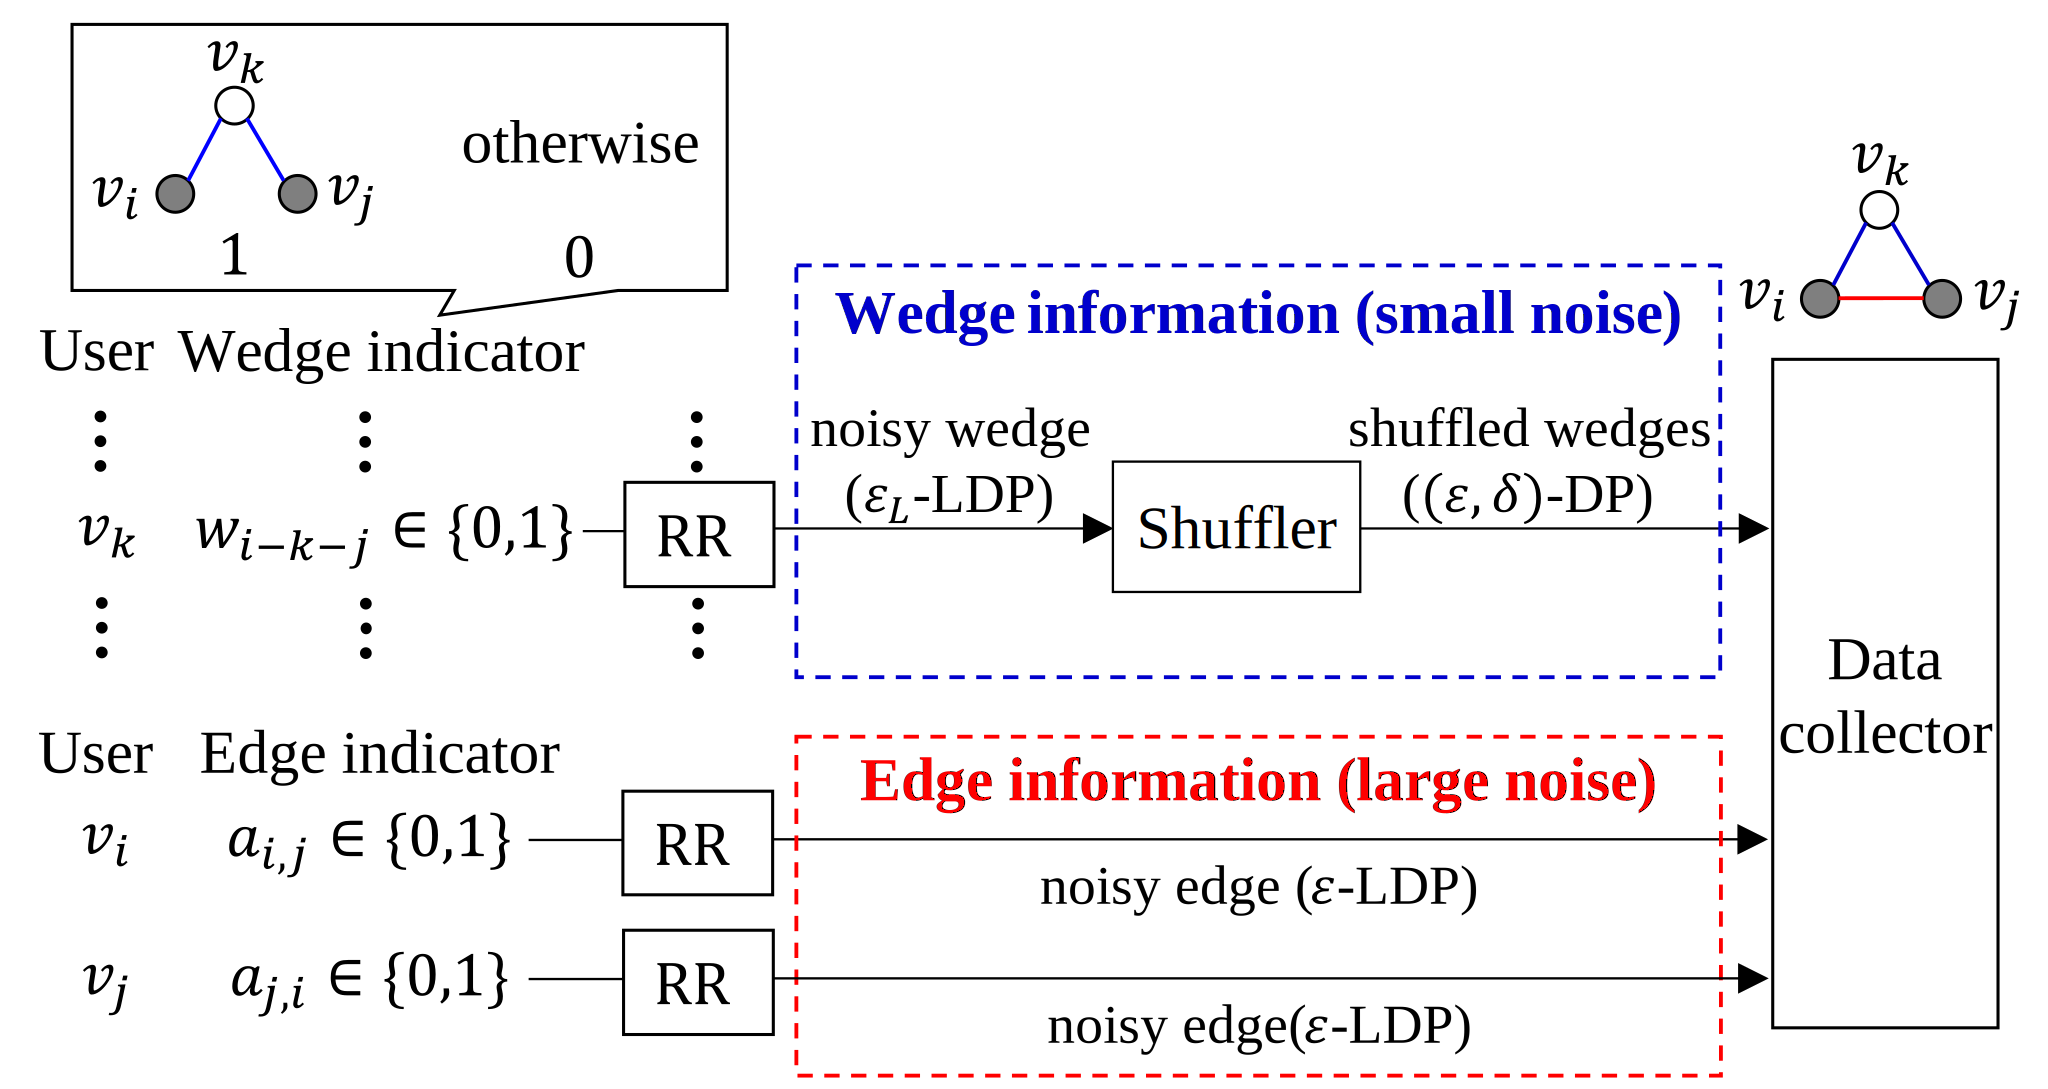
\includegraphics[width=0.99\linewidth]{fig/local_edges.pdf}
  
  \caption{Overview of our \AlgWSLE{} (Wedge Shuffling with Local Edges) algorithm with inputs $v_i$ and $v_j$.
  %our wedge shuffle algorithm with inputs $v_i$ and $v_j$.
  %(marked with gray).
  }
  \label{chap3-fig:local_edges}
% \end{figure}
\vspace{2mm}
% \begin{figure}[t]
  \centering
  \includegraphics[width=0.7\linewidth]{fig/sampling_pairs2.pdf}
  
  \caption{Overview of our triangle counting algorithm.
  We use our
  %wedge shuffle
  \AlgWSLE{}
  algorithm with each user-pair.
  %Independent pairs of nodes do share common nodes, e.g., $(v_1, v_3)$, $(v_2, v_6)$, $(v_4, v_5)$.
  }
  \label{chap3-fig:triangle_count}
\end{figure}

\smallskip
\noindent{\textbf{Sending Local Edges.}}~~First, we consider the problem of counting triangles involving a specific user-pair $(v_i, v_j)$ and propose an algorithm to send
% The shuffled wedge indicators tell us the number of common friends of $v_i$ and $v_j$.
% However, the data collector still cannot count triangles, because she does not know whether $v_i$ and $v_j$ are friends.
% Thus, our wedge shuffle algorithm sends
\textit{local edges} between $v_i$ and $v_j$, along with shuffled wedges, to the data collector.
We call this the \AlgWSLE{} (Wedge Shuffling with Local Edges) algorithm.
%algorithm \AlgWSLE{} (Wedge Shuffle Edge Local).
% the \textit{wedge shuffling with local edges} algorithm and abbreviate it to \AlgWSLE{}.

Figure~\ref{chap3-fig:local_edges} shows the overview of \AlgWSLE{}.
In this algorithm, users $v_i$ and $v_j$ obfuscate edge indicators $a_{i,j}$ and $a_{j,i}$, respectively, using $\epsilon$-RR and send them to the data collector directly (or through the shuffler without shuffling).
%\footnote{It is also possible to send the noisy edge indicators from users $v_i$ and $v_j$ to the data collector through the shuffler. In this case, the shuffler does not shuffle these data.}.
Then, the data collector calculates an unbiased estimate of the triangle count
% from the noisy data.
from the shuffled wedges and the noisy edges.
Because $\epsilon$ is small, a large amount of noise is added to the edge indicators.
However, \textit{only one edge} is noisy (the other two have little noise) in any triangle the data collector sees.
This brings us an advantage over the one-round local algorithms in which all three edges are noisy.

\smallskip
\noindent{\textbf{Sampling Disjoint User-Pairs.}}~~Next, we consider the problem of counting triangles in the entire graph $G$.
A naive solution to this problem is to use our
%wedge shuffling
\AlgWSLE{} algorithm
with all $\binom{n}{2}$ user-pairs as input.
However, it results in very large $\epsilon$ and $\delta$ because it uses each element of the adjacency matrix $\bmA$ many times.
To address this issue,
% To accurately count them under DP,
we propose a triangle counting algorithm that samples
% independent edges (a.k.a. matching), which have no nodes in common.
disjoint user-pairs, ensuring that no user falls in two pairs. 
% which share no common users.
% and then uses the wedge shuffling algorithm for each sampled edge.

Figure~\ref{chap3-fig:triangle_count} shows the overview of our triangle algorithm.
The data collector sends the sampled user-pairs to users.
Then, users apply
%our wedge shuffling algorithm
\AlgWSLE{}
with each user-pair
% as input
and send the results to the data collector.
Finally, the data collector calculates an unbiased estimate of the triangle count from the results.
% This can be viewed as edge sampling \cite{Bera_KDD20,Eden_FOCS15,Wu_TKDE16} in triangle counting.
% Edge sampling is known as an efficient sampling method that outperforms other sampling methods such as node sampling and triangle sampling \cite{Wu_TKDE16}.
% Our triangle counting algorithm is also efficient and
% In fact,
Because our triangle algorithm uses each element of
% the adjacency matrix
$\bmA$ \textit{at most once}, it provides $(\epsilon,\delta)$-element DP hence $(2\epsilon,2\delta)$-edge DP.
In addition, our triangle algorithm reduces the time complexity from $O(n^3)$ to $O(n^2)$ by sampling user-pairs rather than using all user-pairs.
% In addition, our wedge shuffle algorithm with a user-pair $(v_i,v_j)$ provides $(\epsilon,\delta)$-DP for each row in the $i$-th and $j$-th columns of the adjacency matrix $\bmA$, and our triangle algorithm samples independent user-pairs.
% Thus, our algorithm provides $(\epsilon,\delta)$-element DP hence $(2\epsilon,2\delta)$-edge DP.

We prove that the MSE of our triangle counting algorithm is
% $O(n^3 d_{max}^2)$.
$O(n^3)$ when we ignore the factor of $d_{max}$.
% when we regard $\epsilon$ and $\delta$ as constants.
When we do not shuffle wedges, the
% expected
MSE is
% $O(n^5)$.
$O(n^4)$.
% This is much smaller than the existing one-round local algorithm with the same time complexity, whose $l_2$ loss is $O(n^5)$, as shown in Section~\ref{chap3-sub:upper}.
In addition, the MSE of the existing one-round local algorithm \cite{Imola_USENIX22} with the same time complexity is $O(n^6)$, as proved in
\conference{the full version \cite{Imola_CCSFull22}}\arxiv{
Appendix~\ref{chap3-sec:upper}}.
% Section~\ref{chap3-sub:upper}.
% Thus, our algorithm has a much smaller estimation error than the local algorithm.
Thus, our
% wedge shuffling
algorithm
provides a dramatic improvement over the local algorithms.

\smallskip
\noindent{\textbf{Variance Reduction.}}~~Although our
% wedge shuffling
algorithm
dramatically
% reduces
improves
the MSE, the factor of $n^3$ may still be large.
Therefore, we propose a variance reduction technique that ignores sparse user-pairs, where either of the two users has a very small degree.
Our basic idea is that the number of triangles involving such a user-pair is very small
% such user-pairs have a very small number of triangles
and can be approximated by $0$.
By ignoring the sparse user-pairs, we can significantly reduce the variance at the cost of introducing a small bias.
We prove that our variance reduction technique reduces the MSE from $O(n^3)$ to $O(n^\gamma)$ where $\gamma\in[2,3)$ and makes one-round triangle counting more accurate.
%accurate one-round triangle counting possible.
% This enables us to accurately count triangles within one round.


% \subsection{Triangle Counting Including a Specific User-Pair}
% \label{chap3-sub:triangle_edge}
% \subsection{Wedge Shuffling with Local Edges}
\subsection{WSLE (Wedge Shuffling with Local Edges)}
% \subsection{Sending Local Edges}
\label{chap3-sub:wedge}
% Each user $v_k$ ($k \ne i, j$) calculates wedge information $w_{i-k-j} \in \{0,1\}$ that takes $1$ if there is a two-hop path $v_i-v_k-v_j$ and 0 otherwise.
% Then $v_k$ obfuscates $w_{i-k-j}$ using $\epsilon_L$-RR and sends the noisy wedge to the shuffler.
% The shuffler randomly shuffles the noisy wedges to provide $(\epsilon, \delta)$-DP with $\epsilon \ll \epsilon_L$ and sends them to the data collector.
% In addition, users $v_i$ and $v_j$ obfuscate edge information $a_{i,j}$ and $a_{j,i}$, respectively, using $\epsilon$-RR and directly send them to the data collector.

% \smallskip
\noindent{\textbf{Algorithm.}}~~We first
%Consider the problem of counting triangles including a specific user-pair $(v_i,v_j)$.
% To solve this problem, we
propose
% a wedge shuffle algorithm,
the \AlgWSLE{} algorithm
as a building block of our triangle counting algorithm.
\AlgWSLE{} counts
% which estimates the number of
triangles involving a specific user-pair $(v_i,v_j)$.
% We denote this algorithm by \AlgWSLE{}.

Algorithm~\ref{chap3-alg:WSLE} shows \AlgWSLE{}.
% This algorithm estimates the number of triangles including a specific user-pair $(v_i,v_j)$.
Let $f_{i,j}^\triangle: \calG \rightarrow \nnints$ be a function that takes $G \in \calG$ as input and outputs the number $f_{i,j}^\triangle(G)$ of triangles involving $(v_i,v_j)$ in $G$.
Let $\hf_{i,j}^\triangle(G) \in \reals$ be an estimate of $f_{i,j}^\triangle(G)$.
% Let $I_{-(i,j)}$ be the set of indices of users other than $v_i$ and $v_j$, i.e., $I_{-(i,j)} = [n]\setminus\{i,j\}$.

\setlength{\algomargin}{5mm}
\begin{algorithm}[t]
  \SetAlgoLined
  \KwData{Adjacency matrix $\bmA \in \{0,1\}^{n \times n}$,
    %Neighbor lists $\bma_1, \ldots, \bma_n \in \{0,1\}^n$,
    %$\epsilon_L \in \nnreals$, $\delta \in [0,1]$, $\epsilon = f(n-2, \epsilon_L, \delta)$,
    $\epsilon \in \nnreals$, $\delta \in [0,1]$,
    user-pair $(v_i,v_j)$.
  }
  \KwResult{Estimate $\hf_{i,j}^\triangle(G)$ of the number $f_{i,j}^\triangle(G)$ of triangles involving $(v_i,v_j)$.}
  %of the count of triangles including $(v_i,v_j)$.}
%   $I_{-(i,j)} \leftarrow [n]\setminus\{i,j\}$\;
%   $q_L \leftarrow \frac{1}{e^{\epsilon_L}+1}$; $q \leftarrow
  %   \frac{1}{e^\epsilon+1}$\;
  $\epsilon_L \leftarrow \texttt{LocalPrivacyBudget}(n,\epsilon,\delta)$\;
%   $\{y_{\pi(k)} | k \in I_{-(i,j)}\} \leftarrow$ \AlgWS{}$(\bmA, \epsilon, \delta, (v_{\sigma(i)}, v_{\sigma(i+1)}))$\;
  \tcc{Wedge shuffling}
  $\{y_{\pi(k)} | k \in I_{-(i,j)}\} \leftarrow$ \AlgWS{}$(\bmA, \epsilon_L, (v_i, v_j))$\;
  \tcc{Send local edges}
%   \For{$i=1$ \KwTo $n$}{
%   \ForEach{$k \in I_{-(i,j)}$}{
%     [$v_k$] $w_{i-k-j} \leftarrow a_{k,i} a_{k,j}$\;
%     [$v_k$] $y_k \leftarrow \calR_{\epsilon_L}^W(x)(w_{i-k-j})$\;
%     [$v_k$] Send $y_k$ to the shuffler\;
%   }
  [$v_i$] $z_i \leftarrow \calR_{\epsilon}^W(x)(a_{i,j})$; Send $z_i$ to the data collector\;
  [$v_j$] $z_j \leftarrow \calR_{\epsilon}^W(x)(a_{j,i})$; Send $z_j$ to the data collector\;
%   \tcc{Shuffler}
%   [s] Sample a random permutation $\pi$ over $I_{-(i,j)}$\;
%   [s] Send $\{y_{\pi(k)} | k \in I_{-(i,j)}\}$ to the data collector\;
  \tcc{Calculate an unbiased estimate}
  [d] $q_L \leftarrow \frac{1}{e^{\epsilon_L}+1}$; $q \leftarrow
  \frac{1}{e^\epsilon+1}$\;
  [d] $\hf_{i,j}^\triangle(G) \leftarrow \frac{(z_i+z_j-2q)\sum_{k \in
  I_{-(i,j)}} (y_{k} - q_L)}{2(1-2q)(1-2q_L)}$\;
  [d] \KwRet{$\hf_{i,j}^\triangle(G)$}
  \caption{\AlgWSLE{}
  %Our wedge shuffle algorithm
  (Wedge Shuffling with Local Edges).
  \AlgWS{} is shown in Algorithm~\ref{chap3-alg:WShuffle}.
  %[$v_i$], [s], and [d] represent that the process is run by user $v_i$, the shuffler, and the data collector, respectively.
  % Lines 1 and 2 are run by all parties.
  }\label{chap3-alg:WSLE}
\end{algorithm}

% Given $\epsilon$ and $\delta$,
We first call the function \texttt{LocalPrivacyBudget}, which calculates a local privacy budget $\epsilon_L$ from $n$, $\epsilon$, and $\delta$ (line 1).
Specifically, this function calculates $\epsilon_L$
such that $\epsilon$ is a closed-form upper bound (i.e., $\epsilon = f(n-2, \epsilon_L, \delta)$ in (\ref{chap3-eq:shuffle_epsilon_f})) or numerical upper bound in the shuffle model with $n-2$ users.
% \cite{Feldman_FOCS21}.
Given $\epsilon_L$, we can easily calculate the closed-form or numerical upper bound $\epsilon$ by (\ref{chap3-eq:shuffle_epsilon}) and the open source code in \cite{Feldman_FOCS21}\footnote{\url{https://github.com/apple/ml-shuffling-amplification}.}, respectively.
Thus, we can also easily calculate $\epsilon_L$ from $\epsilon$ by calculating a lookup table for pairs $(\epsilon, \epsilon_L)$ in advance.

Then, we run our wedge shuffle algorithm \AlgWS{} in Algorithm~\ref{chap3-alg:WShuffle} (line 2); i.e., each user $v_k \in I_{-(i,j)}$ sends her obfuscated wedge indicator
% obfuscates $w_{i-k-j}$ using $\epsilon_L$-RR $\calR_{\epsilon_L}^W$ and sends the result
$y_k = \calR_{\epsilon_L}^W(w_{i-k-j})$ to the shuffler, and the shuffler sends
shuffled wedge indicators $\{y_{\pi(k)} | k \in I_{-(i,j)}\}$ to the data collector.
%calculates a wedge indicator $w_{i-k-j} \in \{0,1\}$ from her neighbor list $\bma_k$ as follows: $w_{i-k-j} = a_{k,i} a_{k,j}$.
%User $v_k$
% (lines 4-6).
Meanwhile, user $v_i$ obfuscates her edge indicator $a_{i,j}$ using $\epsilon$-RR $\calR_{\epsilon}^W$ and sends the result $z_i = \calR_{\epsilon}^W(a_{i,j})$ to the data collector
% \footnotemark[1]
(line 3).
Similarly, $v_j$ sends $z_j = \calR_{\epsilon}^W(a_{j,i})$ to the data collector (line 4).

% The shuffler samples a uniform random permutation $\pi$ over $I_{-(i,j)}$ and shuffles the wedge indicators based on $\pi$.
% Then, the shuffler sends the shuffled wedge indicators $\{y_{\pi(k)} | k \in I_{-(i,j)}\}$ to the data collector (lines 12-13).

% After receiving $\{y_{\pi(k)} | k \in I_{-(i,j)}\}$, $z_i$, and $z_j$,
Finally, the data collector estimates $f_{i,j}^\triangle(G)$ from $\{y_{\pi(k)} | k \in I_{-(i,j)}\}$, $z_i$, and $z_j$.
% Specifically, let $\hf_{i,j}^\triangle(G) \in \reals$ be an estimate of $f_{i,j}^\triangle(G)$.
Specifically, the data collector calculates the estimate $\hf_{i,j}^\triangle(G)$ as follows:
\begin{align}
    \textstyle{\hf_{i,j}^\triangle(G) = \frac{(z_i+z_j-2q)\sum_{k \in I_{-(i,j)}} (y_{k} -
    q_L)}{2(1-2q)(1-2q_L)},}
    \label{chap3-eq:hfij_triangle}
\end{align}
where $q_L = \frac{1}{e^{\epsilon_L}+1}$ and $q = \frac{1}{e^\epsilon+1}$ (lines 5-6).
Note that this estimate involves simply summing over the set $\{y_{\pi(k)}\}$ and does not require knowing the value of $\pi$. This is
consistent with the shuffle model.
As we prove later, $\hf_{i,j}^\triangle(G)$ in (\ref{chap3-eq:hfij_triangle}) is an unbiased estimate of $f_{i,j}^\triangle(G)$.

\smallskip
\noindent{\textbf{Theoretical Properties.}}~~Below, we show some theoretical properties of \AlgWSLE{}.
% First, we prove that \AlgWSLE{} provides DP:
% \begin{theorem}
% \label{chap3-thm:DP_I}
% \AlgWSLE{} provides $(\epsilon, \delta)$-element DP and $(2\epsilon, 2\delta)$-edge DP.
% \end{theorem}
% Intuitively, Theorem~\ref{chap3-thm:DP_I} comes from the fact that \AlgWSLE{} uses only the $i$-th and $j$-th columns of the adjacency matrix $\bmA$ and protects each element with $(\epsilon,\delta)$-DP.
% See Appendix~\ref{chap3-sec:triangle_proof} for details.
%
% Next,
First, we prove that
the estimate $\hf_{i,j}^\triangle(G)$
% of \AlgWSLE{}
is unbiased:
\begin{theorem}
\label{chap3-thm:unbiased_I}
  For any indices $i,j \in [n]$, the estimate produced by
  $\AlgWSLE{}$ satisfies $\E[\hf_{i,j}^\triangle(G)] = f_{i,j}^\triangle(G)$.
% \AlgWSLE{} provides an unbiased estimate, i.e.,
% \begin{align*}
% \E[\hf_{i,j}^\triangle(G)] = f_{i,j}^\triangle(G).
% \end{align*}
\end{theorem}

% Finally,
Next,
we show the MSE ($=$ variance). 
% of \AlgWSLE{}.
% $\hf_{i,j}^\triangle(G)$.
Recall that in the shuffle model, $\epsilon_L = \log n + O(1)$ when $\epsilon$ and $\delta$ are constants.
%see Section~\ref{chap3-sub:shuffle}
We show
% the expected $l_2$ losses for a general case and the case where $\epsilon_L = \Theta(\log n)$:
the MSE for a general case and for the shuffle model:
\begin{theorem}
\label{chap3-thm:l2-loss_I}
  For any indices $i,j \in [n]$, the estimate produced by
  \AlgWSLE{} provides the following utility guarantee:
% In \AlgWSLE{},
\begin{align}
& \MSE(\hf_{i,j}^\triangle(G)) = \V[\hf_{i,j}^\triangle(G)] \nonumber\\
  & \leq \frac{n q_L + q(1-2q_L)^2 d_{max}^2}{(1-2q)^2(1-2q_L)^2} \triangleq
  err_{\AlgWSLE}(n,d_{max},q,q_L).
\label{chap3-eq:l2_I_general}
\end{align}
  When $\epsilon$ and $\delta$ are constants and $\epsilon_L = \log n + O(1)$, we
  have
\begin{align}
  & err_{\AlgWSLE{}}(n,d_{max}, q, q_L) = O(d_{max}^2).
\label{chap3-eq:l2_I_shuffle}
\end{align}
\end{theorem}
The equation (\ref{chap3-eq:l2_I_shuffle}) follows from (\ref{chap3-eq:l2_I_general}) because $q_L = \frac{1}{e^{\epsilon_L}+1} = \frac{1}{n e^{O(1)} + 1}$. 
% Theorem~\ref{chap3-thm:l2-loss_I} states that
Because \AlgWSLE{} is a building block for our triangle counting algorithms, we
introduce the notation $err_{\AlgWSLE{}}(n,d_{max}, q, q_L)$ for our upper bound
in~\eqref{chap3-eq:l2_I_general}. Observing
\eqref{chap3-eq:l2_I_general}, if we do not use the shuffling technique (i.e.,
$\epsilon_L = \epsilon$), then $err_{\AlgWSLE{}}(n,d_{max}, q, q_L) = O(n + d_{max}^2)$ when we
treat $\epsilon$ and $\delta$ as constants.
In contrast, in the shuffle model where we have $\epsilon_L = \log n + O(1)$,
then $err_{\AlgWSLE{}}(n,d_{max}, q, q_L) = O(d_{max}^2)$.
This means that wedge shuffling reduces the MSE from $O(n + d_{max}^2)$ to $O(d_{max}^2)$, which is significant when $d_{max} \ll n$.

% \subsection{Triangle Counting Based on Wedge Shuffle}
% \subsection{Wedge Shuffle-Based Triangle Counting}
% \subsection{WSLE-Based Triangle Counting}
\subsection{Triangle Counting}
% \subsection{Sampling Independent User-Pairs}
\label{chap3-sub:triangle}
\noindent{\textbf{Algorithm.}}~~Based on
%Now, we turn our attention to the problem of counting triangles in the entire graph $G$ and propose a triangle counting algorithm
% Our wedge shuffle algorithm \AlgWSLE{} estimates the number of triangles including a specific user-pair $(v_i,v_j)$.
% Based on
% this,
\AlgWSLE{},
we propose an algorithm that counts triangles in the entire graph $G$.
We denote this algorithm by \AlgWSTri{}, as it applies wedge shuffling to triangle counting.

Algorithm~\ref{chap3-alg:wshuffle_triangle} shows \AlgWSTri{}.
First, the data collector samples disjoint user-pairs, 
ensuring that no user falls in two pairs. 
% which share no common users.
Specifically, it calls the function \texttt{RandomPermutation}, which samples a uniform random permutation $\sigma$ over $[n]$ (line 1).
Then, it samples disjoint user-pairs as
$(v_{\sigma(1)}, v_{\sigma(2)}), (v_{\sigma(3)}, v_{\sigma(4)}), \ldots, (v_{\sigma(2t-1)}, \allowbreak v_{\sigma(2t)})$, where $t \in [\lfloor \frac{n}{2} \rfloor]$.
The parameter $t$ represents the number of user-pairs and controls the trade-off between the MSE and the time complexity;
when $t = \lfloor \frac{n}{2} \rfloor$, the MSE is minimized and the time complexity is maximized.
The data collector sends the sampled user-pairs to users (line 2).

\setlength{\algomargin}{5mm}
\begin{algorithm}[t]
  \SetAlgoLined
  \KwData{Adjacency matrix $\bmA \in \{0,1\}^{n \times n}$, $\epsilon \in \nnreals$, $\delta \in [0,1]$, $t \in [\lfloor \frac{n}{2} \rfloor]$.
  }
  \KwResult{Estimate $\hf^\triangle(G)$ of $f^\triangle(G)$.}
%   \tcc{Data collector}
  \tcc{Sample disjoint user-pairs}
  [d] $\sigma \leftarrow$\texttt{RandomPermutation}$(n)$\;
  [d] Send $(v_{\sigma(1)}, v_{\sigma(2)}), \ldots, (v_{\sigma(2t-1)}, v_{\sigma(2t)})$ to users\;
%  \ForEach{$i \in \{1, 3, \ldots, 2t-1\}$}{
%    [$d$] Send $(\sigma(i), \sigma(i+1))$ to users\;
%  }
%   \tcc{Users, shuffler, and data collector}
%   \tcc{Wedge shuffling with local edges}
  \ForEach{$i \in \{1, 3, \ldots, 2t-1\}$}{
    $\hf_{\sigma(i), \sigma(i+1)}^\triangle(G) \leftarrow$ \AlgWSLE{}$(\bmA, \epsilon, \delta, (v_{\sigma(i)}, v_{\sigma(i+1)}))$\;
  }
%   \tcc{Data collector}
  \tcc{Calculate an unbiased estimate}
  [d] $\hf^\triangle(G) \leftarrow \frac{n(n-1)}{6t} \sum_{i=1, 3, \ldots, 2t-1} \hf_{\sigma(i),\sigma(i+1)}^\triangle(G)$\;
  [d] \KwRet{$\hf^\triangle(G)$}
  \caption{Our triangle counting algorithm \AlgWSTri{}.
  %Our wedge shuffle-based triangle counting algorithm \AlgWSTri{}.
  %[d] represents that the process is run by the data collector.
  \AlgWSLE{} is shown in Algorithm~\ref{chap3-alg:WSLE}.
  }\label{chap3-alg:wshuffle_triangle}
\end{algorithm}

Then, we run our wedge algorithm \AlgWSLE{} in Algorithm~\ref{chap3-alg:WSLE} with each sampled user-pair as input (lines 3-5).
Finally, the data collector estimates the triangle count $f^\triangle(G)$ as follows:
\begin{align}
    \textstyle{\hf^\triangle(G) = \frac{n(n-1)}{6t} \sum_{i=1, 3, \ldots, 2t-1} \hf_{\sigma(i),\sigma(i+1)}^\triangle(G)}
   \label{chap3-eq:hf_triangle_II}
\end{align}
(line 6). 
Note that a single triangle is never counted by more than one user-pair, as the user-pairs never overlap. 
Later, we prove that $\hf^\triangle(G)$ in (\ref{chap3-eq:hf_triangle_II}) is unbiased.

\smallskip
\noindent{\textbf{Theoretical Properties.}}~~We prove that
% our triangle counting algorithm
\AlgWSTri{} provides DP:
% Below, we show the privacy and utility of \AlgWSTri{}.
% We first prove that \AlgWSTri{} provides DP:
\begin{theorem}
\label{chap3-thm:DP_II}
\AlgWSTri{} provides $(\epsilon, \delta)$-element DP and $(2\epsilon, 2\delta)$-edge DP.
\end{theorem}
Theorem~\ref{chap3-thm:DP_II} comes from the fact that
\AlgWSLE{} with a user-pair $(v_i,v_j)$ provides $(\epsilon,\delta)$-DP for each element in the $i$-th and $j$-th columns of the adjacency matrix $\bmA$ and that \AlgWSTri{} samples disjoint user-pairs, i.e., it uses each element of $\bmA$ at most once.
% and protect each element with $(\epsilon,\delta)$-DP.

Note that running \AlgWSLE{} with all $\binom{n}{2}$ user-pairs 
% requires a very large privacy budget --
% By composition,
% it 
provides $((n-2) \epsilon, (n-2) \delta)$-DP, as it uses each element of $\bmA$ at most $n-2$ times.
The privacy budget is very large, even using the advanced composition \cite{DP,Kairouz_ICML15}.
We avoid this issue by sampling user-pairs that share no common users.

We also prove that
% the estimate of \AlgWSTri{} is unbiased:
\AlgWSTri{} provides an unbiased estimate:
% Next, we show the utility of \AlgWSTri{}:
\begin{theorem}
\label{chap3-thm:unbiased_II}
The estimate produced by \AlgWSTri{} satisfies $\allowbreak \E[\hf^\triangle(G)] = f^\triangle(G)$.
% \AlgWSTri{} provides an unbiased estimate, i.e.,
% \begin{align*}
% \E[\hf^\triangle(G)] = f^\triangle(G).
% \end{align*}
\end{theorem}

Next, we analyze the MSE ($=$ variance) of \AlgWSTri{}.
This analysis is 
% complicated 
non-trivial 
because \AlgWSTri{} samples each user-pair \textit{without replacement}.
In this case, the sampled user-pairs are not independent.
However, we can prove that
$t$ estimates in (\ref{chap3-eq:hf_triangle_II}) are negatively correlated with each other (\conference{see the full version \cite{Imola_CCSFull22} for details}\arxiv{Lemma~\ref{chap3-lem:sampling_replacement_var} in Appendix~\ref{chap3-sub:l2-loss_II_proof}}).
%the covariance of two estimates $\hf_{\sigma(i),\sigma(i+1)}^\triangle(G)$ and $\hf_{\sigma(j),\sigma(j+1)}^\triangle(G)$ in (\ref{chap3-eq:hf_triangle_II})
Thus, the variance of the sum of $t$ estimates
%$\sum_{i=1, 3, \ldots, 2t-1} \hf_{\sigma(i),\sigma(i+1)}^\triangle(G)$
in (\ref{chap3-eq:hf_triangle_II}) is upper bounded by the sum of their variances, each of which is given by Theorem~\ref{chap3-thm:l2-loss_I}.
This brings us to the following result:

\begin{theorem}
\label{chap3-thm:l2-loss_II}
The estimate produced by \AlgWSTri{} provides the following utility guarantee:
\begin{align}
& \MSE(\hf^\triangle(G)) = \V[\hf^\triangle(G)] \nonumber\\
  &\leq
  \frac{n^4}{36t}err_{\AlgWSLE{}}(n,d_{max},q,q_L) +
  \frac{n^3}{36t}d_{max}^3, \label{chap3-eq:thm:l2_II}
\end{align}
where $err_{\AlgWSLE{}}(n,d_{max},q,q_L)$ is given by (\ref{chap3-eq:l2_I_general}).
  When $\epsilon$ and $\delta$ are constants,  $\epsilon_L = \log(n) + O(1)$, and
  $t = \lfloor\frac{n}{2}\rfloor$, we have
\begin{align}
\MSE(\hf^\triangle(G))
  &\leq
  O(n^3d_{max}^2). \label{chap3-eq:thm:l2_II_simp}
\end{align}
\end{theorem}
% Theorem~\ref{chap3-thm:unbiased_II} states that the estimate of \AlgWSTri{} is unbiased.

The inequality (\ref{chap3-eq:thm:l2_II_simp}) follows from (\ref{chap3-eq:l2_I_shuffle}) and (\ref{chap3-eq:thm:l2_II}). 
The first and second terms in~(\ref{chap3-eq:thm:l2_II}) are caused by
% the randomness in
Warner's RR
% for local edges
and the sampling of disjoint user-pairs, respectively.
In other words, the MSE of \AlgWSTri{} can be decomposed into two factors: the RR
% for local edges
and user-pair sampling.

For example, assume that $t = \lfloor \frac{n}{2} \rfloor$.
When we do not shuffle wedges (i.e., $\epsilon_L = \epsilon$), then
$err_{\AlgWSLE{}}(n,d_{max},q,q_L) = O(n + d_{max}^2)$, and
MSE in (\ref{chap3-eq:thm:l2_II}) is $O(n^4 + n^3 d_{max}^2)$.
When we shuffle wedges, the MSE is $O(n^3 d_{max}^2)$.
Thus, when we ignore the factor of $d_{max}$, our wedge shuffle technique reduces the MSE from $O(n^4)$ to $O(n^3)$ in triangle counting.
The factor of $n^3$ is caused by the RR for local edges.
This is intuitive because a large amount of noise is added to the local edges.

Finally, we analyze the time complexity of \AlgWSTri{}.
The time complexity of running \AlgWSLE{} with all $\binom{n}{2}$ user-pairs is $O(n^3)$, as there are $O(n^2)$ user-pairs in total and \AlgWSLE{} requires the time complexity of $O(n)$.
In contrast, the time complexity of \AlgWSTri{} with $t = \lfloor \frac{n}{2} \rfloor$ is $O(n^2)$ because it samples $O(n)$ user-pairs.
Thus, \AlgWSTri{} reduces the time complexity from $O(n^3)$ to $O(n^2)$ by user-pair sampling.
We can further reduce the time complexity at the cost of increasing the MSE by setting $t$ small,
% the number $t$ of sampled user-pairs small,
i.e., $t \ll \lfloor \frac{n}{2} \rfloor$.
% However, it comes at the cost of increasing the $l_2$ loss.

% \subsection{Variance Reduction Based on Ignoring Sparse User-Pairs}
\subsection{Variance Reduction}
\label{chap3-sub:var_red}
\noindent{\textbf{Algorithm.}}~~\AlgWSTri{}
% Our triangle counting algorithm \AlgWSTri{}
achieves the MSE of $O(n^3)$ when we ignore the factor of $d_{max}$.
% However, the factor of $n^3$ is still large because the square of the true count $f^\triangle(G)$ is $O(n^2)$.
% To provide a small relative error, we want to reduce the $l_2$ loss of \AlgWSTri{} from $O(n^3)$ to at most $O(n^2)$.
% To this end,
To provide a smaller estimation error,
we propose a variance reduction technique that ignores sparse user-pairs.
We denote our triangle counting algorithm with the variance reduction technique by \AlgWSTriVR{}.

% Let $d_{i,j} = \min\{d_i, d_j\}$ be the minimum degree of users $v_i$ and $v_j$.
As explained in Section~\ref{chap3-sub:triangle}, the factor of $n^3$ is caused by the RR for local edges.
However, most user-pairs $v_i$ and $v_j$ have a very small minimum degree
% $d_{i,j} \ll d_{max}$,
$\min\{d_i, d_j\} \ll d_{max}$,
and there is no edge $(v_i, v_j)$ between them in almost all cases.
In addition, even if there is an edge $(v_i, v_j)$, the number of triangles involving the sparse user-pair is very small
% (at most $d_{i,j}-1$)
(at most $\min\{d_i, d_j\}$)
and can be approximated by $0$.
% Thus,
% we can approximate the number of triangles including the sparse user-pair by $0$.
By ignoring such sparse user-pairs, we can dramatically reduce the variance of the RR for local edges at the cost of a small bias.
This is an intuition behind our variance reduction technique.

% Specifically, we consider the following improvement of \AlgWSTri{}.
% Let $d_{i,j} = \min\{d_i, d_j\}$ be the minimum degree of users $v_i$ and $v_j$.
% Below, we assume that the data collector knows each user $v_i$'s degree $d_i$ for ease of explanation.
% Note that $d_i$ can leak the information about edges of $v_i$.
% Thus, we explain how to privately estimate $d_i$ with edge DP within one-round at the end of Section~\ref{chap3-sub:var_red}.
Algorithm~\ref{chap3-alg:wshuffle_triangle_vr} shows \AlgWSTriVR{}.
This algorithm detects sparse user-pairs based on the degree information.
However, user $v_i$'s degree $d_i$ can leak the information about edges of $v_i$.
Thus, \AlgWSTriVR{} calculates a differentially private estimate of $d_i$ within one round.

\setlength{\algomargin}{5mm}
\begin{algorithm}[t]
  \SetAlgoLined
  \KwData{Adjacency matrix $\bmA \in \{0,1\}^{n \times n}$, $\epsilon_1, \epsilon_2 \in \nnreals$, $\delta \in [0,1]$, $t \in [\lfloor \frac{n}{2} \rfloor]$, $c \in \nnreals$.
  }
  \KwResult{Estimate $\hf^\triangle(G)$ of $f^\triangle(G)$.}
%   \tcc{Data collector}
  \tcc{Sample disjoint user-pairs}
  [d] $\sigma \leftarrow$\texttt{RandomPermutation}$(n)$\;
  [d] Send $(v_{\sigma(1)}, v_{\sigma(2)}), \ldots, (v_{\sigma(2t-1)}, v_{\sigma(2t)})$ to users\;
%   \tcc{Users, shuffler, and data collector}
%   \tcc{Wedge shuffling with local edges}
  \ForEach{$i \in \{1, 3, \ldots, 2t-1\}$}{
    $\hf_{\sigma(i), \sigma(i+1)}^\triangle(G) \leftarrow$ \AlgWSLE{}$(\bmA, \epsilon_2, \delta, (v_{\sigma(i)}, v_{\sigma(i+1)}))$\;
  }
%   \tcc{Users}
  \tcc{Send noisy degrees}
  \For{$i=1$ \KwTo $n$}{
    [$v_i$] $\td_i \leftarrow d_i + \Lap(\frac{1}{\epsilon_1})$; Send $\td_i$ to the data collector\;
  }
%   \tcc{Data collector}
  \tcc{Calculate a variance-reduced estimate}
%   [d] $d_{th} \leftarrow \frac{c}{n} \sum_{i=1}^n \td_i$\;
  [d] $\td_{avg} \leftarrow \frac{1}{n} \sum_{i=1}^n \td_i$; $d_{th} \leftarrow c \td_{avg}$\;
  [d] $D \leftarrow \{i | i = 1, 3, \ldots, 2t-1,
  \min\{\td_{\sigma(i)}, \td_{\sigma(i+1)}\} > d_{th}\}$\;
  [d] $\hf^\triangle(G) \leftarrow \frac{n(n-1)}{6t} \sum_{i \in D} \hf_{\sigma(i),\sigma(i+1)}^\triangle(G)$\;
  [d] \KwRet{$\hf^\triangle(G)$}
  \caption{Our triangle counting algorithm with variance reduction \AlgWSTriVR{}.
  %[$v_i$] and [d] represent that the process is run by user $v_i$ and the data collector, respectively.
  \AlgWSLE{} is shown in Algorithm~\ref{chap3-alg:WSLE}.
  }\label{chap3-alg:wshuffle_triangle_vr}
\end{algorithm}

Specifically, \AlgWSTriVR{} uses two privacy budgets: $\epsilon_1, \epsilon_2 \in \nnreals$.
The first budget $\epsilon_1$ is for privately estimating $d_i$, whereas the second budget $\epsilon_2$ is for
\AlgWSLE{}.
% wedge shuffling.
Lines 1 to 5 in Algorithm~\ref{chap3-alg:wshuffle_triangle_vr} are the same as those in Algorithm~\ref{chap3-alg:wshuffle_triangle}, except that Algorithm~\ref{chap3-alg:wshuffle_triangle_vr} uses $\epsilon_2$
% rather than $\epsilon$.
to provide $(\epsilon_2, \delta)$-element DP.
After these processes, each user $v_i$ adds the Laplacian noise $\Lap(\frac{1}{\epsilon_1})$ with mean $0$ and scale $\frac{1}{\epsilon_1}$ to her degree $d_i$ and sends the noisy degree $\td_i$ ($= d_i + \Lap(\frac{1}{\epsilon_1})$) to the data collector (lines 6-8).
% Since adding or removing one element changes $d_i$ by at most $1$
Because the sensitivity \cite{DP} of $d_i$ (the maximum distance of $d_i$ between two neighbor lists that differ in one bit) is $1$, adding $\Lap(\frac{1}{\epsilon_1})$ to $d_i$ provides $\epsilon_1$-element DP.

Then, the data collector estimates the average degree $d_{avg}$ as $\td_{avg} = \frac{1}{n}\sum_{i=1}^n \td_i$ and sets a threshold $d_{th}$ of the minimum degree to $d_{th} = c \td_{avg}$, where $c \in \nnreals$ is a small positive number, e.g.,
% $c=1$ or $2$
$c \in [1,10]$ (line 9).
% (line 10).
%$c \in \nnints$ times the private estimate $\frac{1}{n} \sum_{i=1}^n \td_i$ of $d_{avg}$ (line 10).
Finally, the data collector estimates $f^\triangle(G)$ as
%follows:
\begin{align}
    \textstyle{\hf^\triangle(G) = \frac{n(n-1)}{6t} \sum_{i \in D} \hf_{\sigma(i),\sigma(i+1)}^\triangle(G),}
   \label{chap3-eq:hf_triangle_II_ast}
\end{align}
where
\begin{align*}
D = \{i | i = 1, 3, \ldots, 2t-1,
  \min\{\td_{\sigma(i)}, \td_{\sigma(i+1)}\} > d_{th}\}
\end{align*}
(lines 10-11).
The difference between (\ref{chap3-eq:hf_triangle_II}) and (\ref{chap3-eq:hf_triangle_II_ast}) is that (\ref{chap3-eq:hf_triangle_II_ast}) ignores sparse user-pairs $v_{\sigma(i)}$ and $v_{\sigma(i+1)}$ such that $\min\{\td_{\sigma(i)}, \td_{\sigma(i+1)}\} \leq d_{th}$.
% Because
Since
$d_{avg} \ll d_{max}$ in practice,
% $\min\{\td_{\sigma(i)}, \td_{\sigma(i+1)}\} \ll d_{max}$
$d_{th} \ll d_{max}$
holds for small $c$.

The parameter $c$ controls the trade-off between the bias and variance of the estimate $\hf^\triangle(G)$.
The larger $c$ is, the more user-pairs are ignored.
Thus, as $c$ increases, the bias is increased, and the variance is reduced.
% Although the optimization of $c$ is challenging and is left for future work,
In practice,
%$c=1$ or $2$
%$c \in [1,10]$
a small $c$ not less than $1$ 
%(e.g., $c \in [1,10]$)
results in a small MSE % for the following reasons.
% First, the bias is small in this case because $c d_{avg} \ll d_{max}$.
% Second,
% Note that
because most real graphs are scale-free networks that have a power-law degree distribution \cite{NetworkScience}.
% where
In the scale-free networks, most users' degrees are smaller than the average degree $d_{avg}$.
For example, in the BA (Barab\'{a}si-Albert) graph model \cite{NetworkScience,Hagberg_SciPy08},
most users' degrees are $\frac{d_{avg}}{2}$.
% with parameter (number of edges per node) $m$, the average degree is $d_{avg} = 2m$ and most users' degrees are $m$.
Thus, if we set
% $c \geq 1$,
%$c=1$ or $2$,
% (e.g., $c=1$ or $2$),
$c \in [1,10]$, for example,
then most user-pairs are ignored (i.e., $|D| \ll t$), which leads to a significant reduction of the variance at the cost of a small bias.
% In our experiments, we set $c=1$.

Recall that the parameter $t$ in \AlgWSTriVR{} controls the trade-off between the MSE and the time complexity. 
Although \AlgWSTriVR{} always samples $t$ disjoint user-pairs, we can modify \AlgWSTriVR{} so that it stops sampling user-pairs right after the estimate $\hf^\triangle(G)$ in (\ref{chap3-eq:hf_triangle_II_ast}) is converged. 
We can also sample dense user-pairs $(v_i, v_j)$ with large noisy degrees $\td_i$ and $\td_j$ at the beginning (e.g., by sorting users in descending order of noisy degrees) to improve the MSE for small $t$. 
Evaluating such improved algorithms is left for future work. 

\smallskip
\noindent{\textbf{Theoretical Properties.}}~~As with \AlgWSTri{},
\AlgWSTriVR{} provides the following privacy guarantee:
%\AlgWSTriVR{} also provides DP:

\begin{theorem}
\label{chap3-thm:DP_II_ast}
\AlgWSTriVR{} provides $(\epsilon_1 + \epsilon_2, \delta)$-element DP and $(2(\epsilon_1 + \epsilon_2), 2\delta)$-edge DP.
\end{theorem}

Next, we analyze the bias of \AlgWSTriVR{}. Here, we assume most users have a small degree 
using parameters $\lambda \in \nnreals$ and $\alpha \in [0,1)$: 
% Under this assumption, we can show that the set $D$ truly consists of vertex
% pairs such that $d_{i} \geq d_{th}$, and that the noisy estimates $\hd_i$ do not
% result in a ``noisy'' $D$ where $d_i \geq d_{th}$ is often not true. We can then control the bias
% by observing that vertices with high degree are not excluded from $D$.
% As explained above, we use the ideas
% that there are not many edges involving users with degree less than $d_{th}$, and
% that ignoring estimates in which one user has such a low degree will only
% discard up to $d_{th}$ triangles.
% For this theorem and the next,
% let
% $\overline{d}_{th} = cd_{avg} + \frac{7(c+1)\log n}{\epsilon_1}$ and
% $\underline{d}_{th} = cd_{avg} - \frac{7(c+1)\log n}{\epsilon_1}$.
% The $\log n$ terms arise due to
% adding the Laplacian noise to obtain
% the private degrees $\td_{i}$, and they are much smaller than $c d_{avg}$ in
% most applications.

\begin{theorem}
\label{chap3-thm:bias_II_ast}
  Suppose that in $G$, there exist $\lambda \in \nnreals$ and $\alpha \in [0,1)$
  such that at most $n^\alpha$ users have a degree larger than
  $\lambda d_{avg}$. Suppose \AlgWSTriVR{} is run with $c \geq \lambda$.
  Then, the estimator produced by
  \AlgWSTriVR{} provides the following bias guarantee:
\begin{align}
    Bias[\hf^\triangle(G)]
    = |\E[\hf^\triangle(G)] - f^\triangle(G)|
    \leq
    \frac{n c^2 d_{avg}^2}{3} +
    %\frac{1}{3}n(c d_{avg})^2 +
    \frac{4 n^\alpha}{3 \epsilon_1^2}.
    %\frac{1}{3} n^\alpha \left(\frac{2}{\epsilon_1}\right)^2.
    \label{chap3-eq:thm:bias_II_ast}
\end{align}
\end{theorem}
% The bias in (\ref{chap3-eq:thm:bias_II_ast}) depends on $\lambda$ $\alpha$
The values of $\lambda$ and $\alpha$ depend on the original graph $G$.
In the scale-free networks, $\alpha$ is small for a moderate value of $\lambda$.
For example, in the BA graph with $n=107614$ and $d_{avg}=200$ used in \conference{the full version \cite{Imola_CCSFull22}}\arxiv{Appendix~\ref{chap3-sec:BA-graph}}, $\alpha = 0.5$, $0.6$, $0.8$, and $0.9$ when $\lambda = 10.1$, $5.4$, $1.6$, and $0.9$, respectively.
When $c$ and $\epsilon_1$ are constants,
% Since $\alpha \in [0,1]$,
% In Theorem~\ref{chap3-thm:bias_II_ast}, the $\log n$ term arises due to the Laplacian noise $\Lap(\frac{1}{\epsilon_1})$ to obtain
% the private degree $\td_{i}$.
% Note that $\log n$ is much smaller than $d_{avg}$ in most graph data, e.g., $(\log n, d_{avg}) = (11.6, \allowbreak 227.4)$ or $(13.7, 127.3)$ in our experiments.
% applications.
% Thus, when $c$ is small (e.g., $c=1$ or $2$),
the bias can be expressed as $O(n d_{avg}^2)$.
% by regarding the parameter $c$ as a constant.
% by ignoring the factor of
% $d_{avg}$ ($\ll d_{max}$).

Finally, we show the variance of \AlgWSTriVR{}. 
This result assumes that $c$ is bigger $(= \frac{(1-\alpha) \log n}{\epsilon_1 d_{avg}})$ than $\lambda$. 
%This is necessary 
We assume this 
because otherwise, many sparse users (with $d_i \leq \lambda d_{avg}$) have a noisy degree $\td_i \geq c \td_{avg}$, causing the set $D$ to
be noisy. In practice, the gap between $c$ and $\lambda$ is small because 
$\log n$ is much smaller than $d_{avg}$. 
% Our theorem will use the value

% $K$, the number of nodes in $G$ with degree greater than
% $\underline{d}_{th}$. In practice, this quantity is much less than $O(n)$

\begin{theorem}
\label{chap3-thm:var_II_ast}
  Suppose that in $G$, there exist $\lambda \in \nnreals$ and $\alpha \in [0,1)$
  such that at most $n^\alpha$ users have a degree larger than
  $\lambda d_{avg}$. Suppose \AlgWSTriVR{} is
  run with $c \geq \lambda + \frac{(1-\alpha) \log n}{\epsilon_1 d_{avg}}$.
  Then, the estimator produced by
  \AlgWSTriVR{} provides the following variance guarantee:
\begin{align}
  &\V[\hf^\triangle(G)] \leq \nonumber\\
  &\frac{n^2 d_{max}^4}{9} + \frac{2n^{2+2\alpha}}{9t}err_{\AlgWSLE}(n,d_{max},q,q_L) + \frac{n^{2+\alpha}
  d_{max}^3 }{36t}.
%   &\frac{n^2 d_{max}^4}{9} + \frac{n^{2+2\alpha}}{6t}err_{\AlgWSLE}(n,d_{max},q,q_L) + \frac{n^{2+\alpha}
%   d_{max}^3 }{36t}.
  \label{chap3-eq:thm:l2_II_ast}
\end{align}
When $\epsilon_1$, $\epsilon_2$, and $\delta$ are constants,
% $\alpha$ satisfies $\alpha < \frac{1}{2}$, and
$\epsilon_L = \log n + O(1)$, and $t = \lfloor\frac{n}{2}\rfloor$,
% then
\begin{align}
%   \V[\hf_*^\triangle(G)] \leq O(n^2 d_{max}^4).
  \V[\hf^\triangle(G)] \leq O(n^2 d_{max}^4 + n^{1+2\alpha} d_{max}^2).
  \label{chap3-eq:thm:l2_II_ast_simp}
\end{align}
\end{theorem}

% \colorB{Finally, we show the variance of \AlgWSTriVR{}.
% For simplicity, we assume that we do not add the Laplacian noise to $d_i$, i.e., $\td_i = d_i$.
% This assumption is fine because $\Lap(\frac{1}{\epsilon_1})$ is very small in practice -- we show that adding $\Lap(\frac{1}{\epsilon_1})$ hardly affects the estimation error in our experiments.
% Under this assumption, we show the variance:}
%
% \begin{theorem}
% \label{chap3-thm:var_II_ast_wo_Lap}
% \colorB{The estimate produced by \AlgWSTriVR{} without the Laplacian noise ($\td_i = d_i$ for $i\in[n]$) provides the following variance guarantee:
% \begin{align}
% \V[\hf^\triangle(G)] \leq
%   \frac{|D|n^4}{36t^2}err_{\AlgWSLE{}}(n,d_{max},q,q_L) +
%   \frac{|D|n^3}{36t^2}d_{max}^3, \label{chap3-eq:thm:l2_II_ast_wo_Lap}
% \end{align}
% where $err_{\AlgWSLE{}}(n,d_{max},q,q_L)$ is given by (\ref{chap3-eq:l2_I_general}).
%   When $\epsilon$ and $\delta$ are constants,  $\epsilon_L = \log(n) + O(1)$, and
%   $t = \lfloor\frac{n}{2}\rfloor$, we have
% \begin{align}
% l_2^2(f^\triangle(G), \hf^\triangle(G))
%   &\leq
%   O(|D|n^2d_{max}^2). \label{chap3-eq:thm:l2_II_ast_wo_Lap_simp}
% \end{align}}
% \end{theorem}

% The first term in (\ref{chap3-eq:thm:l2_II_ast}) comes from the Laplacian noise $\Lap(\frac{1}{\epsilon_1})$ to obtain
% the private degree $\td_i$.
% The latter two terms are similar to those
% of~\eqref{chap3-eq:thm:l2_II}.
% \colorR{In practice, $K$ is much less than $n$}.
% Since $K \ll n$, the second term
% in~\eqref{chap3-eq:thm:l2_II_ast_simp} is $O(n)$ (ignoring $d_{max},K$ factors), as
% opposed to $O(n^3)$ which \AlgWSTri{} suffers from.
% $O(n^2 d_{max}^2 (|D| + d_{max}))$.
% Thus, when we ignore the factor of $d_{max}$ and $K$,
% (both of which are much smaller than $n$),
The first\footnote{The first term in (\ref{chap3-eq:thm:l2_II_ast}) is actually $\frac{(\sum_{i=1}^n d_i^2)^2}{9}$ and is much smaller than $\frac{n^2 d_{max}^4}{9}$. 
We express it as $O(n^2 d_{max}^4)$ in (\ref{chap3-eq:thm:l2_II_ast_simp}) for simplicity. 
See \conference{the full version \cite{Imola_CCSFull22}}\arxiv{Appendix~\ref{chap3-sub:var_II_ast_proof}} for details.}, second, and third terms in (\ref{chap3-eq:thm:l2_II_ast}) are caused by the randomness in the choice of $D$, the RR, and user-pair sampling, respectively. 
By (\ref{chap3-eq:thm:l2_II_ast_simp}), our variance reduction technique reduces the variance from $O(n^3)$ to $O(n^\gamma)$ where $\gamma\in[2,3)$ when we ignore the factor of $d_{max}$.
Because the MSE is the sum of the squared bias and the variance, it is also $O(n^\gamma)$.

The value of $\gamma$ in our bound $O(n^\gamma)$ depends on the parameter $c$ in \AlgWSTriVR{}.
For example, in the BA graph ($n=107614$, $d_{avg} = 200$), $\gamma=2$, $2.2$, $2.6$, and $2.8$ ($\alpha=0.5$, $0.6$, $0.8$, and $0.9$) when $c=10.4$, $5.6$, $1.7$, and $1.0$, respectively, and $\epsilon_1=0.1$.
Thus, the variance decreases with increase in $c$.
However, by (\ref{chap3-eq:thm:bias_II_ast}), a larger $c$ results in a larger bias. 
In our experiments, we show that \AlgWSTriVR{} provides a small estimation error when $c=1$ to $4$.
When $c=1$, \AlgWSTriVR{} empirically works well despite a large $\gamma$ because most users' degrees are smaller than $d_{avg}$ in practice, as explained above.
This indicates that our upper bound in (\ref{chap3-eq:thm:l2_II_ast_simp}) might not be tight when $c$ is around $1$.
Improving the bound is left for future work.

% our technique reduces the variance from $O(n^3)$ to $O(n^2)$.
% Because the expected $l_2$ loss is the summation of the squared bias and the variance, it can also be expressed as $O(n^2)$.

% \commentT{$K$ can be $n$, e.g., in our experiments using \IMDB{}, $\epsilon_1=0.1$, $n=896308$, $d_{avg}=127.3$, and $c=1$. In this case, $\underline{d}_{th} = 127.3 - 1918.8 < 0$.}

\subsection{Summary}
\label{chap3-sub:summary}

Table~\ref{chap3-tab:upper_bounds_triangle} summarizes the
performance guarantees
% upper bounds
of one-round triangle algorithms providing edge DP.
Here,
% In \AlgWSTriVR{}, we regard $c$ as a constant (e.g., $c=1$ or $2$) and assume that $d_{th} = O(d_{avg})$.
we consider a variant of \AlgWSTri{} that does not shuffle wedges (i.e., $\epsilon_L = \epsilon$) as a one-round local algorithm.
We call this variant \AlgWLTri{} (Wedge Local).
% We also show \AlgARRTri{} \cite{Imola_USENIX22} and \AlgRRTri{} \cite{Imola_USENIX21} as existing one-round local algorithms.
We also show the variance of \AlgARRTri{} \cite{Imola_USENIX22} and \AlgRRTri{} \cite{Imola_USENIX21}.
The time complexity of \AlgRRTri{} is $O(n^3)$\footnote{Technically speaking, the algorithms of \AlgRRTri{} and
the one-round local algorithms in \cite{Ye_ICDE20,Ye_TKDE21} involve counting the number of triangles in a dense
graph. This can be done in time $O(n^\omega)$, where $\omega \in [2,3)$ and $O(n^\omega)$ is the time required for matrix multiplication. However, these algorithms are of theoretical interest,
and they do not outperform naive matrix multiplication except
for very large matrices~\cite{Alman_2021}. Thus, we assume implementations that use naive matrix multiplication in
$O(n^3)$ time.}, and that
% The time complexity
of \AlgARRTri{} is $O(n^2)$ when we set the sampling probability $p_0 \in [0,1]$ of the ARR to $p_0=O(n^{-1/3})$.
We prove the variance of \AlgARRTri{} in this case and \AlgRRTri{}
% We prove the variance of \AlgARRTri{} \cite{Imola_USENIX22} and \AlgRRTri{} \cite{Imola_USENIX21}
%as existing one-round local algorithms.
in \conference{the full version \cite{Imola_CCSFull22}}\arxiv{Appendix~\ref{chap3-sec:upper}}.
We do not show the other one-round local algorithms \cite{Ye_ICDE20,Ye_TKDE21} in Table~\ref{chap3-tab:upper_bounds_triangle} for two reasons: (i) they have the time complexity of $O(n^3)$ and suffer from a larger estimation error than \AlgRRTri{} \cite{Imola_USENIX22};
% it is reported in \cite{Imola_USENIX22} that they are outperformed by \AlgRRTri{};
(ii) their upper-bounds on the variance and bias are unclear.

\begin{table}[t]
  \caption{Performance guarantees
  %Upper bounds
  of one-round triangle counting algorithms providing edge DP.
  %``Time'' represents the time complexity.
  $\alpha \in [0,1)$. 
  See also footnote 2 for the variance of \AlgWSTriVR{}.
  %$K \ll n$ in practice.
  }
  
  \centering
%   \begin{tabular}{|l|c|c|}
%     \hline
%     Algorithm & $l_2$ loss & Time complexity \\ \hline
%     \AlgWSTri{} & $O(n^3 d_{max}^2)$ & $O(n^2)$ \\ \hline
%     \AlgWSTriVR{}{} & $O(n^2 d_{max}^2 + n^2 d_{th}^4)$ & $O(n^2)$ \\ \hline
%     \AlgWLTri{} & $O(n^4 + n^3 d_{max}^2)$ & $O(n^2)$ \\ \hline
%     \AlgARRTri{} & $O(n^5)$ & $O(n^2)$ \\ \hline
%     \AlgRRTri{} & $O(n^4)$ & $O(n^3)$ \\ \hline
%   \end{tabular}
  \begin{tabular}{|l|c|c|c|c|}
    \hline
    Algorithm & \hspace{-0.8mm}Model\hspace{-0.8mm} & Variance & Bias & Time \\ \hline
    % \multirow{2}{*}{\AlgWSTriVR{}} & \multirow{2}{*}{shuffle} & \hspace{-1mm}$O(n^2
    % d_{max}^4 \hspace{-0.5mm}+\hspace{-0.5mm} n^{1+2\alpha} d_{max}^2$\hspace{-1mm} & \multirow{2}{*}{\hspace{-1.5mm}$O(n d_{avg}^2)$\hspace{-1.5mm}} & \multirow{2}{*}{$O(n^2)$}
    % \\ & & $ + n^{1+\alpha} d_{max}^3)$ & & 
    \AlgWSTriVR{} & \hspace{-0.8mm}shuffle\hspace{-0.8mm} & \hspace{-1mm}$O(n^2
    d_{max}^4 \hspace{-0.5mm}+\hspace{-0.5mm} n^{1+2\alpha} d_{max}^2)$\hspace{-1mm} & \hspace{-1.5mm}$O(n d_{avg}^2)$\hspace{-1.5mm} & $O(n^2)$\\
    \hline
    % \AlgWSTriVR{} & shuffle & $O(n^2 d_{max}^2 (d_{max}+|D|))$ & $O(n^2 d_{avg}^4)$ & $O(n^2)$ \\ \hline
    \AlgWSTri{} & \hspace{-0.8mm}shuffle\hspace{-0.8mm} & $O(n^3 d_{max}^2)$ & $0$ & $O(n^2)$ \\ \hline
    \AlgWLTri{} & local & $O(n^4 + n^3 d_{max}^2)$ & $0$ & $O(n^2)$ \\ \hline
    \AlgARRTri{} \cite{Imola_USENIX22} & local & $O(n^6)$ & $0$ & $O(n^2)$ \\ \hline
    \AlgRRTri{} \cite{Imola_USENIX21} & local & $O(n^4)$ & $0$ & $O(n^3)$ \\ \hline
  \end{tabular}
  \label{chap3-tab:upper_bounds_triangle}
\end{table}

Table~\ref{chap3-tab:upper_bounds_triangle} shows that our \AlgWSTriVR{} dramatically outperforms the three local algorithms -- when we ignore $d_{max}$, the MSE of \AlgWSTriVR{} is 
$O(n^\gamma)$ where $\gamma\in[2,3)$, 
whereas that of the local algorithms is $O(n^4)$ or $O(n^6)$.
We also show this through experiments. 

Note that both \AlgARRTri{} and \AlgRRTri{} provide pure DP ($\delta=0$), whereas our shuffle algorithms provide approximate DP ($\delta > 0$). 
However, it would not make a noticeable difference, as $\delta$ is sufficiently small (e.g., $\delta = 10^{-8} \ll \frac{1}{n}$ in our experiments). 

\smallskip
\noindent{\textbf{Comparison with the Central Model.}}~~Finally, we note that our \AlgWSTriVR{} is worse than algorithms in the central model in terms of the estimation error. 
% Our shuffle algorithms are preferable to algorithms providing central DP in terms of the trust model -- the central model assumes that a single party accesses personal data of all users and therefore has a risk that the entire graph is leaked from the party. 
% However, our shuffle algorithms are worse than central algorithms in terms of the estimation error. 

Specifically, Imola \textit{et al.} \cite{Imola_USENIX21} consider a central algorithm that 
adds the Laplacian noise $\Lap(\frac{d_{max}}{\varepsilon})$ to the true count $f^\triangle(G)$ and 
outputs $f^\triangle(G) + \Lap(\frac{d_{max}}{\epsilon})$\footnote{Here, we assume that $d_{max}$ is publicly available; e.g., $d_{max}=5000$ in Facebook \cite{Facebook_Limit}. 
When $d_{max}$ is not public, the algorithm in \cite{Imola_USENIX21} outputs $f(G) + \Lap(\frac{\td_{max}}{\epsilon})$, where $\td_{max} = \max_{i=1,\ldots,n} \td_i$, i.e., the maximum of noisy degrees.}. 
% outputs $f(G) + \Lap(\frac{\td_{max}}{\epsilon_2})$. 
% where $\td_{max} = \max_{i=1,\ldots,n} \td_i$ and $\td_i = d_i + \Lap(\frac{1}{\epsilon_1})$. 
This central algorithm provides 
$(\epsilon, 0)$-edge DP. 
% $(2\epsilon_1 + \epsilon_2, 0)$-edge DP. 
In addition, the estimate is unbiased, and the variance is $\frac{2d_{max}^2}{\epsilon^2} = O(d_{max}^2)$. 
Thus, the central algorithm provides a much smaller MSE ($=$ variance) than \AlgWSTriVR{}. 

However, our \AlgWSTriVR{} is preferable to central algorithms in terms of the trust model -- the central model assumes that a single party accesses personal data of all users and therefore has a risk that the entire graph is leaked from the party. 
\AlgWSTriVR{} can also be applied to decentralized social networks, as described in Section~\ref{chap3-sec:intro}. 

% \subsection{Lower Bounds for Local Algorithms}
% \label{chap3-sub:two-rounds}
% TBD

% \subsection{Algorithm}
% \label{chap3-sub:triangle_algorithm}
% TBD

% \subsection{Theoretical Analysis}
% \label{chap3-sub:triangle_theoretical}
% TBD

% \subsection{4-Cycle Counting}
% \label{chap3-sub:4-cycle}
% TBD

%!TEX root=main.tex
\section{4-Cycle Counting Based on Wedge Shuffling}
\label{chap3-sec:4cycle}

Next, we propose a one-round 4-cycle counting algorithm in the shuffle model.
Section~\ref{chap3-sub:4cycle_overview} explains its overview.
Section~\ref{chap3-sub:4cycle_details} proposes our 4-cycle counting algorithm and shows its theoretical properties. 
Section~\ref{chap3-sub:summary_4cycle} summarizes the performance guarantees of our 4-cycle algorithms. 
% The proofs of all statements in this section are given in Appendix~\ref{chap3-sec:4cycle_proof}.

\subsection{Overview}
\label{chap3-sub:4cycle_overview}
% \textbf{Sending Local Wedges}
% To count 4-cycles in the graph based on our wedge shuffling technique, we introduce 
We apply our wedge shuffling technique to 4-cycle counting with two additional techniques: \textit{(i) bias correction} and \textit{(ii) sampling disjoint user-pairs}. 
Below, we briefly explain each of them. 

\smallskip
\noindent{\textbf{Bias Correction.}}~~As with triangles, we begin with the problem of counting 4-cycles involving specific users $v_i$ and $v_j$. 
We can leverage the noisy wedges output by our wedge shuffle algorithm \AlgWS{} to estimate such a 4-cycle count. 
% the number of $4$-cycles
% between two users $v_i, v_j$. 
Specifically, let $f^\square_{i,j}: \calG \rightarrow \nnints$ be a function that, given $G \in \calG$, outputs the number $f^\square_{i,j}(G)$ of $4$-cycles for which users $v_i$ and $v_j$ are opposite nodes, i.e. the number of unordered pairs $(k,k')$ such that $v_i-v_k-v_j-v_{k'}-v_i$ is a path in $G$.
Each pair $(k,k')$ satisfies the above requirement if and only if $v_i-v_k-v_j$ and $v_i-v_{k'}-v_j$ are wedges in $G$.
Thus, we have $f^\square_{i,j}(G) = \binom{f^\wedge_{i,j}}{2}$, where $f^\wedge_{i,j}$ is the number of wedges between $v_i$ and $v_j$. 
Based on this, we calculate an unbiased estimate $\hf^\wedge_{i,j}$ of the wedge count using \AlgWS{}. 
Then, we calculate an estimate of the 4-cycle count as $\binom{\hf^\wedge_{i,j}}{2}$. 
% an unbiased estimate $\hf^\square_{i,j}(G)$ of the 4-cycle count from $\hf^\wedge_{i,j}$. 
Here, it should be noted that the estimate $\binom{\hf^\wedge_{i,j}}{2}$ 
% $\binom{\hf^\wedge_{i,j}}{2}$ 
is \textit{biased}, as proved later. 
%However, $\binom{\hf^\wedge_{i,j}(G)}{2}$ is \textit{not} an unbiased estimate of $f^\square_{i,j}(G)$, as proved later. 
Therefore, 
%Thus, we calculate an unbiased estimate of $f^\square_{i,j}(G)$ via bias correction -- 
we perform bias correction -- we subtract a positive value from the estimate to obtain an unbiased estimate $\hf_{i,j}^\square(G)$ of the 4-cycle count. 

% Because \AlgWS{} can be used to estimate $f^\wedge_{i,j}{2}$, we are able to obtain an estimator $\hf^\square_{i,j}(G)$.
%The estimator is of the form $\binom{\hf^\wedge_{i,j}(G)}{2} - C$, where $C$ is a constant independent of $\hf^\wedge_{i,j}(G)$ that debiases the estimate.
Note that unlike \AlgWSLE{}, no edge between $(v_i,v_j)$ needs to be sent. 
In addition, thanks to the privacy amplification by shuffling, all wedges can be sent with 
% a large $\epsilon$.
small noise.

\smallskip
% \textbf{Sampling Independent User-Pairs} 
\noindent{\textbf{Sampling Disjoint User-Pairs.}}~~Having an estimate $\hf_{i,j}^\square(G)$, we turn our attention to estimating 4-cycle count $f^\square(G)$ in the entire graph $G$.
As with triangles, a naive solution using estimates $\hf_{i,j}^\square(G)$ for all $\binom{n}{2}$ user-pairs $(v_i,v_j)$ results in very large $\epsilon$ and $\delta$. 
To avoid this, we sample disjoint user-pairs and obtain an unbiased estimate of $f^\square(G)$ from them. 
%Naively, we could obtain estimates $\hf_{i,j}^\square(G)$ for all pairs $i,j$, to obtain a concentrated estimate of $\hf^\square(G)$. However, this would not be good for privacy, as each user would send wedge information about all pairs of other vertices, using each value of his adjacency list up to $n$ times. Instead, and identical to the design of \AlgWSTri{}, our algorithm estimates $\hf^\square_{i,j}(G)$ for $t$ disjoint pairs of users with $1 \leq t \leq \lfloor \frac{n}{2} \rfloor$.

\subsection{4-Cycle Counting}
\label{chap3-sub:4cycle_details}

\setlength{\algomargin}{5mm}
\begin{algorithm}[t]
  \SetAlgoLined
  \KwData{Adjacency matrix $\bmA \in \{0,1\}^{n \times n}$, $\epsilon \in \nnreals$, $\delta \in [0,1]$, $t \in [\lfloor \frac{n}{2} \rfloor]$.
  }
  \KwResult{Estimate $\hf^\square(G)$ of $f^\square(G)$.}
  $\epsilon_L \leftarrow \texttt{LocalPrivacyBudget}(n,\epsilon,\delta)$\;
  [d] $q_L \leftarrow \frac{1}{e^{\epsilon_L}+1}$\;
%   \tcc{Data collector}
  \tcc{Sample disjoint user-pairs}
  [d] $\sigma \leftarrow$\texttt{RandomPermutation}$(n)$\;
  [d] Send $(v_{\sigma(1)}, v_{\sigma(2)}), \ldots, (v_{\sigma(2t-1)}, v_{\sigma(2t)})$ to users\;
%  \ForEach{$i \in \{1, 3, \ldots, 2t-1\}$}{
%    [$d$] Send $(\sigma(i), \sigma(i+1))$ to users\;
%  }
%   \tcc{Users, shuffler, and data collector}
%   \tcc{Wedge shuffling}
  \ForEach{$i \in \{1, 3, \ldots, 2t-1\}$}{
    $\{y_{\pi_i(k)} | k \hspace{-1mm}\in I_{-(\sigma(i),\sigma(i+1))}\} \hspace{-1mm}\leftarrow\hspace{-1mm}$ \AlgWS{}$(\bmA, \epsilon_L, (v_{\sigma(i)}, v_{\sigma(i+1)}))$\;
    [d] $\hf_{\sigma(i),\sigma(i+1)}^\wedge(G) \leftarrow \sum_{k \in I_{-(\sigma(i),\sigma(i+1))}} \frac{y_{k} - q_L}{1-2q_L}$\;
    [d] $\hf_{\sigma(i),\sigma(i+1)}^\square(G) \leftarrow  \frac{\hf_{\sigma(i),\sigma(i+1)}^\wedge(G)(\hf_{\sigma(i),\sigma(i+1)}^\wedge(G)-1)}{2} - \frac{n-2}{2}\frac{q_L(1-q_L)}{(1-2q_L)^2}$\;
  }
%   \tcc{Data collector}
  \tcc{Calculate an unbiased estimate}
  [d] $\hf^\square(G) \leftarrow \frac{n(n-1)}{4t}\sum_{i=1,3,\ldots,2t-1} \hf_{\sigma(i),\sigma(i+1)}^\square(G)$\;
  %[d] $\hf^\square(G) \leftarrow \frac{n(n-1)}{4t}\sum_{i=1,3,\ldots,2t-1} \left(\frac{\hf_{\sigma(i),\sigma(i+1)}^\wedge(G)(\hf_{\sigma(i),\sigma(i+1)}^\wedge(G)-1)}{2} - \frac{n-2}{2}\frac{q_L(1-q_L)}{(2q_L-1)^2}\right)$\;
  [d] \KwRet{$\hf^\square(G)$}
  \caption{Our 4-cycle counting algorithm \AlgWSCyc{}.
  %$\hf^\wedge$ is a shorthand for $\hf_{\sigma(i),\sigma(i+1)}^\wedge(G)$.
  \AlgWS{} is shown in Algorithm~\ref{chap3-alg:WShuffle}.
  }\label{chap3-alg:wshuffle_cycle}
\end{algorithm}

\noindent{\textbf{Algorithm.}}~~Algorithm \ref{chap3-alg:wshuffle_cycle} shows our 4-cycle counting algorithm. 
We denote it by \AlgWSCyc{}. 
% Our algorithm \AlgWSCyc{} produces an unbiased estimator $\hf^\square_{i,j}(G)$. 
% The algorithm appears in Algorithm~\ref{chap3-alg:wshuffle_cycle}. 
First, we set a local privacy budget $\epsilon_L$ from $n$, $\epsilon$, and $\delta$ in the same way as \AlgWSLE{} (line 1). 
%line 1 sets $\epsilon_L$ to be a value such that the entire algorithm in the shuffle model achieves $(\epsilon, \delta)$-DP. This value is given by Theorem~\ref{chap3-thm:shuffle}.
%In lines 3-4, 
Then, we sample $t$ disjoint pairs of users using the permutation $\sigma$ (lines 3-4). 
Each pair is given by $(v_{\sigma(i), \sigma(i+1)})$ for $i \in \{1, 3, \ldots, 2t-1\}$.

%In lines 5-9, 
For each $i \in \{1, 3, \ldots, 2t-1\}$, we compute an unbiased estimate $\hf_{\sigma(i),
\sigma(i+1)}^\square(G)$ of the 4-cycle count involving $v_{\sigma(i)}$ and $v_{\sigma(i+1)}$ (lines 5-9). 
To do this, 
%in line 6 
we call \AlgWS{} on
$(v_{\sigma(i)} v_{\sigma(i+1)})$ to obtain an unbiased estimate $\hf_{\sigma(i),
\sigma(i+1)}^\wedge(G)$ of the wedge count (lines 6-7). 
We calculate an estimate $\hf_{i,j}^\wedge(G)$ of the number $f_{i,j}^\wedge(G)$ of wedges between $v_i$ and $v_j$ in $G$ as follows:
% and is given by
\begin{equation}\label{chap3-eq:wedge-estimate}
  \textstyle{\hf^\wedge_{i,j}(G) = \sum_{k \in I_{-(i,j)}} \frac{y_k - q_L}{1-2q_L}.}
\end{equation}
Later, we will prove that $\hf^\wedge_{i,j}(G)$ is an unbiased estimator. 
As with (\ref{chap3-eq:hfij_triangle}), this estimate involves the sum over the set $\{y_{\pi(k)}\}$ and does not require knowing the permutation $\pi$ produced by the shuffler. 
%Note that each permutation $\pi_i$ used to shuffle the data is distinct for each iteration of the loop, and it is unknown to the data collector.
% In line 8, 
Then, we obtain an unbiased estimator of $f_{\sigma(i), \sigma(i+1)}^\square$ as follows:
%, given by
\begin{equation}\label{chap3-eq:4-cycle-ij-estimate}
  \textstyle{\hf_{i,j}^\square(G) = \frac{\hf^\wedge_{i, j}(G)(\hf^\wedge_{i, j}(G)-1)}{2} - \frac{n-2}{2}\frac{q_L(1-q_L)}{(1-2q_L)^2}}
\end{equation}
(line 8). 
Note that 
% even though 
% $\hf_{i, j}^\wedge(G)$ is unbiased, and we have that $f_{i, j}^\square(G) = \binom{f_{i, j}^\wedge(G)}{2}$, 
% because 
there is a quadratic relationship between $f_{i, j}^\square(G)$ and $f_{i, j}^\wedge(G)$, i.e., $f_{i, j}^\square(G) = \binom{f_{i, j}^\wedge(G)}{2}$. 
% the two quantities, 
Thus, 
even though $\hf_{i, j}^\wedge(G)$ is unbiased, 
we must subtract a term from $\binom{\hf_{i, j}^\wedge(G)}{2}$ (i.e., bias correction) to obtain an unbiased estimator $\hf_{i, j}^\square(G)$. 
This forms the righthand side of
~\eqref{chap3-eq:4-cycle-ij-estimate} and ensures that $\hf_{i,j}^\square(G)$ is unbiased. 
% as we prove later.

Finally, 
%in line 10, 
we sum and scale 
% the sample 
$\hf_{\sigma(i), \sigma(i+1)}^\square(G)$ for each $i$ to obtain an estimate $\hf^\square(G)$ of the 4-cycle count $f^\square(G)$ in the entire graph $G$: 
% is summed and scaled by the proper amount to produce an final estimate:

\begin{equation}\label{chap3-eq:4-cycle-estimate}
  \textstyle{\hf^\square(G) = \frac{n(n-1)}{4t}\sum_{i=1,3,\ldots,2t-1} \hf_{\sigma(i),\sigma(i+1)}^\square(G)}
\end{equation}
%The factor $\frac{n(n-1)}{4t}$ serves to scale up the estimate, as only $t$ out of a possible $\binom{n}{2}$ samples of $f_{i,j}^\square(G)$ are estimated.
(line 10). 
% As we prove later, $\hf^\square(G)$ is an unbiased estimate of $f^\square(G)$. 
Note that it is possible that a single 4-cycle is counted twice; e.g., 
% by $\hf_{\sigma(1),\sigma(2)}^\square, \ldots, \hf_{\sigma(2t-1),\sigma(2t)}^\square$. 
a 4-cycle $v_i$-$v_j$-$v_k$-$v_l$-$v_i$ is possibly counted by $(v_i,v_k)$ and $(v_j,v_l)$ if these user-pairs are selected. 
However, this is not an issue, because all 4-cycles are equally likely to be counted zero times, once, or twice. 
We also prove later that $\hf^\square(G)$ in (\ref{chap3-eq:4-cycle-estimate}) is an unbiased estimate of $f^\square(G)$. 

\smallskip
\noindent{\textbf{Theoretical Properties.}}~~First, \AlgWSCyc{} guarantees DP:
% In the same way as \AlgWSTri{}, we can show that 
\begin{theorem}\label{chap3-thm:DP_IV}
\AlgWSCyc{} provides $(\epsilon, \delta)$-element DP and $(2\epsilon, 2\delta)$-edge DP.
\end{theorem}

In addition, thanks to the design of~\eqref{chap3-eq:4-cycle-ij-estimate}, we can show that \AlgWSCyc{} produces an unbiased estimate of $f^\square(G)$:
\begin{theorem}\label{chap3-thm:unbiased_IV}
  The estimate produced by \AlgWSCyc{} satisfies $\allowbreak \E[\hf^\square(G)] =
  f^\square(G)$.
\end{theorem}

Finally, we show the MSE ($=$ variance) of $f^\square(G)$:

\begin{theorem}\label{chap3-thm:l2-loss_IV}
  The estimate produced by \AlgWSCyc{} satisfies 
  \begin{align}
    & \MSE(\hf^\square(G)) = \V[\hf^\square(G)] \nonumber \\
    &\leq \frac{9n^5 q_L(d_{max} +
    nq_L)^2}{16t(1-2q_L)^4} + \frac{n^3d_{max}^6}{64t}. \label{chap3-eq:4-cycle-var}
  \end{align}
  When $\epsilon$ and $\delta$ are constants, $\epsilon_L = \log n + O(1)$, and $t
  = \lfloor \frac{n}{2} \rfloor$, we have
  \begin{equation}\label{chap3-eq:4-cycle-var-simp}
    \MSE(\hf^\square(G)) = \V[\hf^\square(G)] 
    = O\left( n^3 d_{max}^2 + n^2d_{max}^6 \right).
  \end{equation}
\end{theorem}
The first and second terms in (\ref{chap3-eq:4-cycle-var}) are caused by the RR and the sampling of disjoint user-pairs, respectively. 

\begin{table}[t]
  \caption{Performance guarantees of one-round 4-cycle counting algorithms providing edge DP.
  % a``Time'' represents the time complexity.
  }
  \vspace{-4mm}
  \centering
  \begin{tabular}{|l|c|c|c|c|}
    \hline
    Algorithm & Model & Variance & Bias & Time \\ \hline
    \AlgWSCyc{} & shuffle & $O(n^3 d_{max}^2 + n^2 d_{max}^6)$ & $0$ & $O(n^2)$ \\ \hline
    \AlgWLCyc{} & local & $O(n^6 + n^2 d_{max}^6)$ & $0$ & $O(n^2)$ \\ \hline
  \end{tabular}
  \label{chap3-tab:upper_bounds_4cycle}
\end{table}

% \smallskip
% \noindent{\textbf{Summary.}}~~
\subsection{Summary}
\label{chap3-sub:summary_4cycle}
Table~\ref{chap3-tab:upper_bounds_4cycle} summarizes the performance guarantees of the 4-cycle counting algorithms. 
As a one-round local algorithm, we consider a local model version of \AlgWSCyc{} that does not shuffle wedges (i.e., $\epsilon_L = \epsilon$). 
We denote it by \AlgWLCyc{}. 
To our knowledge, \AlgWLCyc{} is the first local 4-cycle counting algorithm. 

By (\ref{chap3-eq:4-cycle-var}), when $t = \lfloor \frac{n}{2} \rfloor$, the MSE of \AlgWLCyc{} can be expressed as $O(n^6 + n^2 d_{max}^6)$. 
Thus, our wedge shuffle technique dramatically reduces the MSE from $O(n^6 + n^2 d_{max}^6)$ to $O(n^3 d_{max}^2 + n^2 d_{max}^6)$. 
Note that the square of the true count $f^\square(G)$ is $O(n^2 d_{max}^6)$. 
This indicates that our \AlgWSCyc{} may not work well in an extremely sparse graph where $d_{max} < n^{\frac{1}{4}}$. 
However, $d_{max} \gg n^{\frac{1}{4}}$ holds in most social graphs; e.g., the maximum number $d_{max}$ of friends is much larger than $100$ when $n=10^8$. 
In this case, \AlgWSCyc{} can accurately estimate the 4-cycle count, as shown in our experiments. 

\smallskip
\noindent{\textbf{Comparison with the Central Model.}}~~As with triangles, our \AlgWSCyc{} is worse than algorithms in the central model in terms of the estimation error. 

Specifically, 
% given that $d_{max}$ is publicly available, 
analogously to the central algorithm for triangles~\cite{Imola_USENIX21}, 
we can consider a central algorithm that outputs $f^\square(G) + \Lap(\frac{d_{max}^2}{\epsilon})$. 
This algorithm provides 
$(\epsilon, 0)$-edge DP and the variance of $\frac{2d_{max}^4}{\epsilon^2} = O(d_{max}^4)$. 
Because $d_{max}$ is much smaller than $n$, this central algorithm provides a much smaller MSE ($=$ variance) than \AlgWSCyc{}. 
% Together with the results in Section~\ref{chap3-sub:summary}, this result suggests 
This indicates 
that there is a trade-off between the trust model and the estimation error. 

% \subsection{Algorithm}
% \label{chap3-sub:4cycle_algorithm}
% TBD

% \subsection{Theoretical Analysis}
% \label{chap3-sub:4cycle_theoretical}
% TBD

% % \section{Lower Bounds}
% \label{sec:lower}
\section{Theoretical Comparison with Local Algorithms}
\label{sec:comp}
TBD

\subsection{Upper Bounds for Local Algorithms}
\label{sub:upper}
Upper bounds for the efficient one-round local algorithm in \cite{Imola_USENIX22}. Here, we do not assume the ER model, unlike \cite{Imola_USENIX21}. 

\subsection{Lower Bounds for Local Algorithms}
\label{sub:lower}
TBD

\subsection{Summary}
\label{sub:comp}
TBD

\section{Experimental Evaluation}
\label{chap3-sec:experiments}
Based on the performance guarantees summarized in Tables~\ref{chap3-tab:upper_bounds_triangle} and \ref{chap3-tab:upper_bounds_4cycle}, we pose the following research questions: 

\begin{description}[leftmargin=8.75mm]
% \begin{description}[leftmargin=9.75mm]
% \begin{itemize}[leftmargin=9.7mm]
    \item[RQ1.] 
    %\item 
    How much do our entire algorithms (\AlgWSTriVR{} and \AlgWSCyc{}) outperform the local algorithms?
    %How much do our shuffle algorithms (\AlgWSTriVR{} and \AlgWSCyc{}) reduce the estimation error, compared to the local algorithms?
    \item[RQ2.] 
    %\item 
    For triangles, how much does our variance reduction technique decrease the relative error?
    \item[RQ3.] 
    %\item 
    How small relative errors do our entire algorithms 
    % (\AlgWSTriVR{} and \AlgWSCyc{}) 
    achieve with a small privacy budget?
\end{description}
% \end{itemize}
We designed experiments to answer these questions. 

\subsection{Experimental Set-up}
\label{chap3-sub:set-up}
We used the following two real graph datasets: 
\begin{itemize}
    \item \textbf{Gplus}: The first dataset is the Google+ dataset \cite{McAuley_NIPS12} denoted by \Gplus{}. 
    %was collected from users who had shared their social circles and whose network information was publicly available. 
    %From this dataset, we 
    This dataset includes a social graph $G=(V,E)$ with $n=107614$ users and $12238285$ edges, where an edge $(v_i, v_j) \in E$ represents that a user $v_i$ follows or is followed by $v_j$. 
    The average and maximum degrees are $d_{avg} = 227.4$ and $d_{max} = 20127$, respectively. 
    \item \textbf{IMDB}: The second dataset is the IMDB (Internet Movie Database)~\cite{IMDB_GD05} denoted by \IMDB{}. 
    This dataset includes a bipartite graph between $896308$ actors and $428440$ movies. 
    From this, we extracted a graph $G=(V,E)$ with $n=896308$ actors and $57064358$ edges, where an edge represents that two actors have played in the same movie. 
    The average and maximum degrees are $d_{avg} = 127.3$ and $d_{max} = 15451$, respectively; i.e., \IMDB{} is more sparse than \Gplus{}. 
\end{itemize}
In \conference{the full version \cite{Imola_CCSFull22}}\arxiv{Appendix~\ref{chap3-sec:BA-graph}}, we also evaluate our algorithms using the Barab\'{a}si-Albert graphs \cite{NetworkScience,Hagberg_SciPy08}, which have a power-law degree distribution. 
Moreover, in \conference{\cite{Imola_CCSFull22}}\arxiv{Appendix~\ref{chap3-sec:bipartite}}, we evaluate our 4-cycle algorithms using bipartite graphs generated from \Gplus{} and \IMDB{}. 

For triangle counting, we evaluated the following four one-round algorithms: \AlgWSTriVR{}, \AlgWSTri{}, \AlgWLTri{}, and \AlgARRTri{} \cite{Imola_USENIX22}. 
We did not evaluate \AlgRRTri{} \cite{Imola_USENIX21}, because it was too inefficient -- it was reported in \cite{Imola_USENIX21} that when $n=10^6$, \AlgRRTri{} would require over $30$ years even on a supercomputer. 
The same applies to the one-round local algorithms in \cite{Ye_ICDE20,Ye_TKDE21} with the same time complexity ($=O(n^3)$). 
% We also evaluated the two-rounds local 

For 4-cycle counting, we compared \AlgWSCyc{} with \AlgWLCyc{}. 
Because \AlgWLCyc{} is the first local 4-cycle counting algorithm (to our knowledge), we did not evaluate other algorithms. 

In our shuffle algorithms \AlgWSTriVR{}, \AlgWSTri{}, and \AlgWSCyc{}, we set $\delta = 10^{-8}$ ($\ll \frac{1}{n}$) and $t=\frac{n}{2}$. 
We used the numerical upper bound in \cite{Feldman_FOCS21} for calculating $\epsilon$ in the shuffle model. 
% In \conference{the full version \cite{Imola_CCSFull22}}\arxiv{Appendix~\ref{chap3-sec:numerical_closed}}, we compare the numerical bound with the closed-form bound in Theorem~\ref{chap3-thm:shuffle}. 
In \AlgWSTriVR{}, we set 
% $c=1$ 
$c\in[0.1,4]$ 
and 
%(as described in Section~\ref{chap3-sub:var_red}) 
divided the total privacy budget $\epsilon$ as $\epsilon_1 = \frac{\epsilon}{10}$ and $\epsilon_2 = \frac{9\epsilon}{10}$. 
Here, we assigned a small budget to $\epsilon_1$ because a degree $d_i$ has a very small sensitivity ($=1$) and $\Lap(\frac{1}{\epsilon_1})$ is very small. 
In \AlgARRTri{}, we set the sampling probability $p_0$ to $p_0 = n^{-1/3}$ or $0.1n^{-1/3}$ so that the time complexity is $O(n^2)$. 

We ran each algorithm $20$ times and evaluated the average relative error over the $20$ runs. 
In \conference{the full version \cite{Imola_CCSFull22}}\arxiv{Appendix~\ref{chap3-sec:standard_error}}, we show that the standard error of the average relative error is small. 

\subsection{Experimental Results}
\label{chap3-sub:results}

% \smallskip
\noindent{\textbf{Relative Error vs. $\epsilon$.}}~~We first evaluated the relation between the relative error and 
% the privacy budget 
$\epsilon$ in element DP or edge LDP, i.e., $2\epsilon$ in edge DP. 
We also measured the time to estimate the triangle/4-cycle count from the adjacency matrix $\bmA$ using a supercomputer \cite{ABCI} with two Intel Xeon Gold 6148 processors (2.40 GHz, 20 Cores) and 412 GB main memory. 
% We implemented each algorithm with C/C++ \cite{GraphShuffle}. 

\begin{figure}[t]
  \centering
  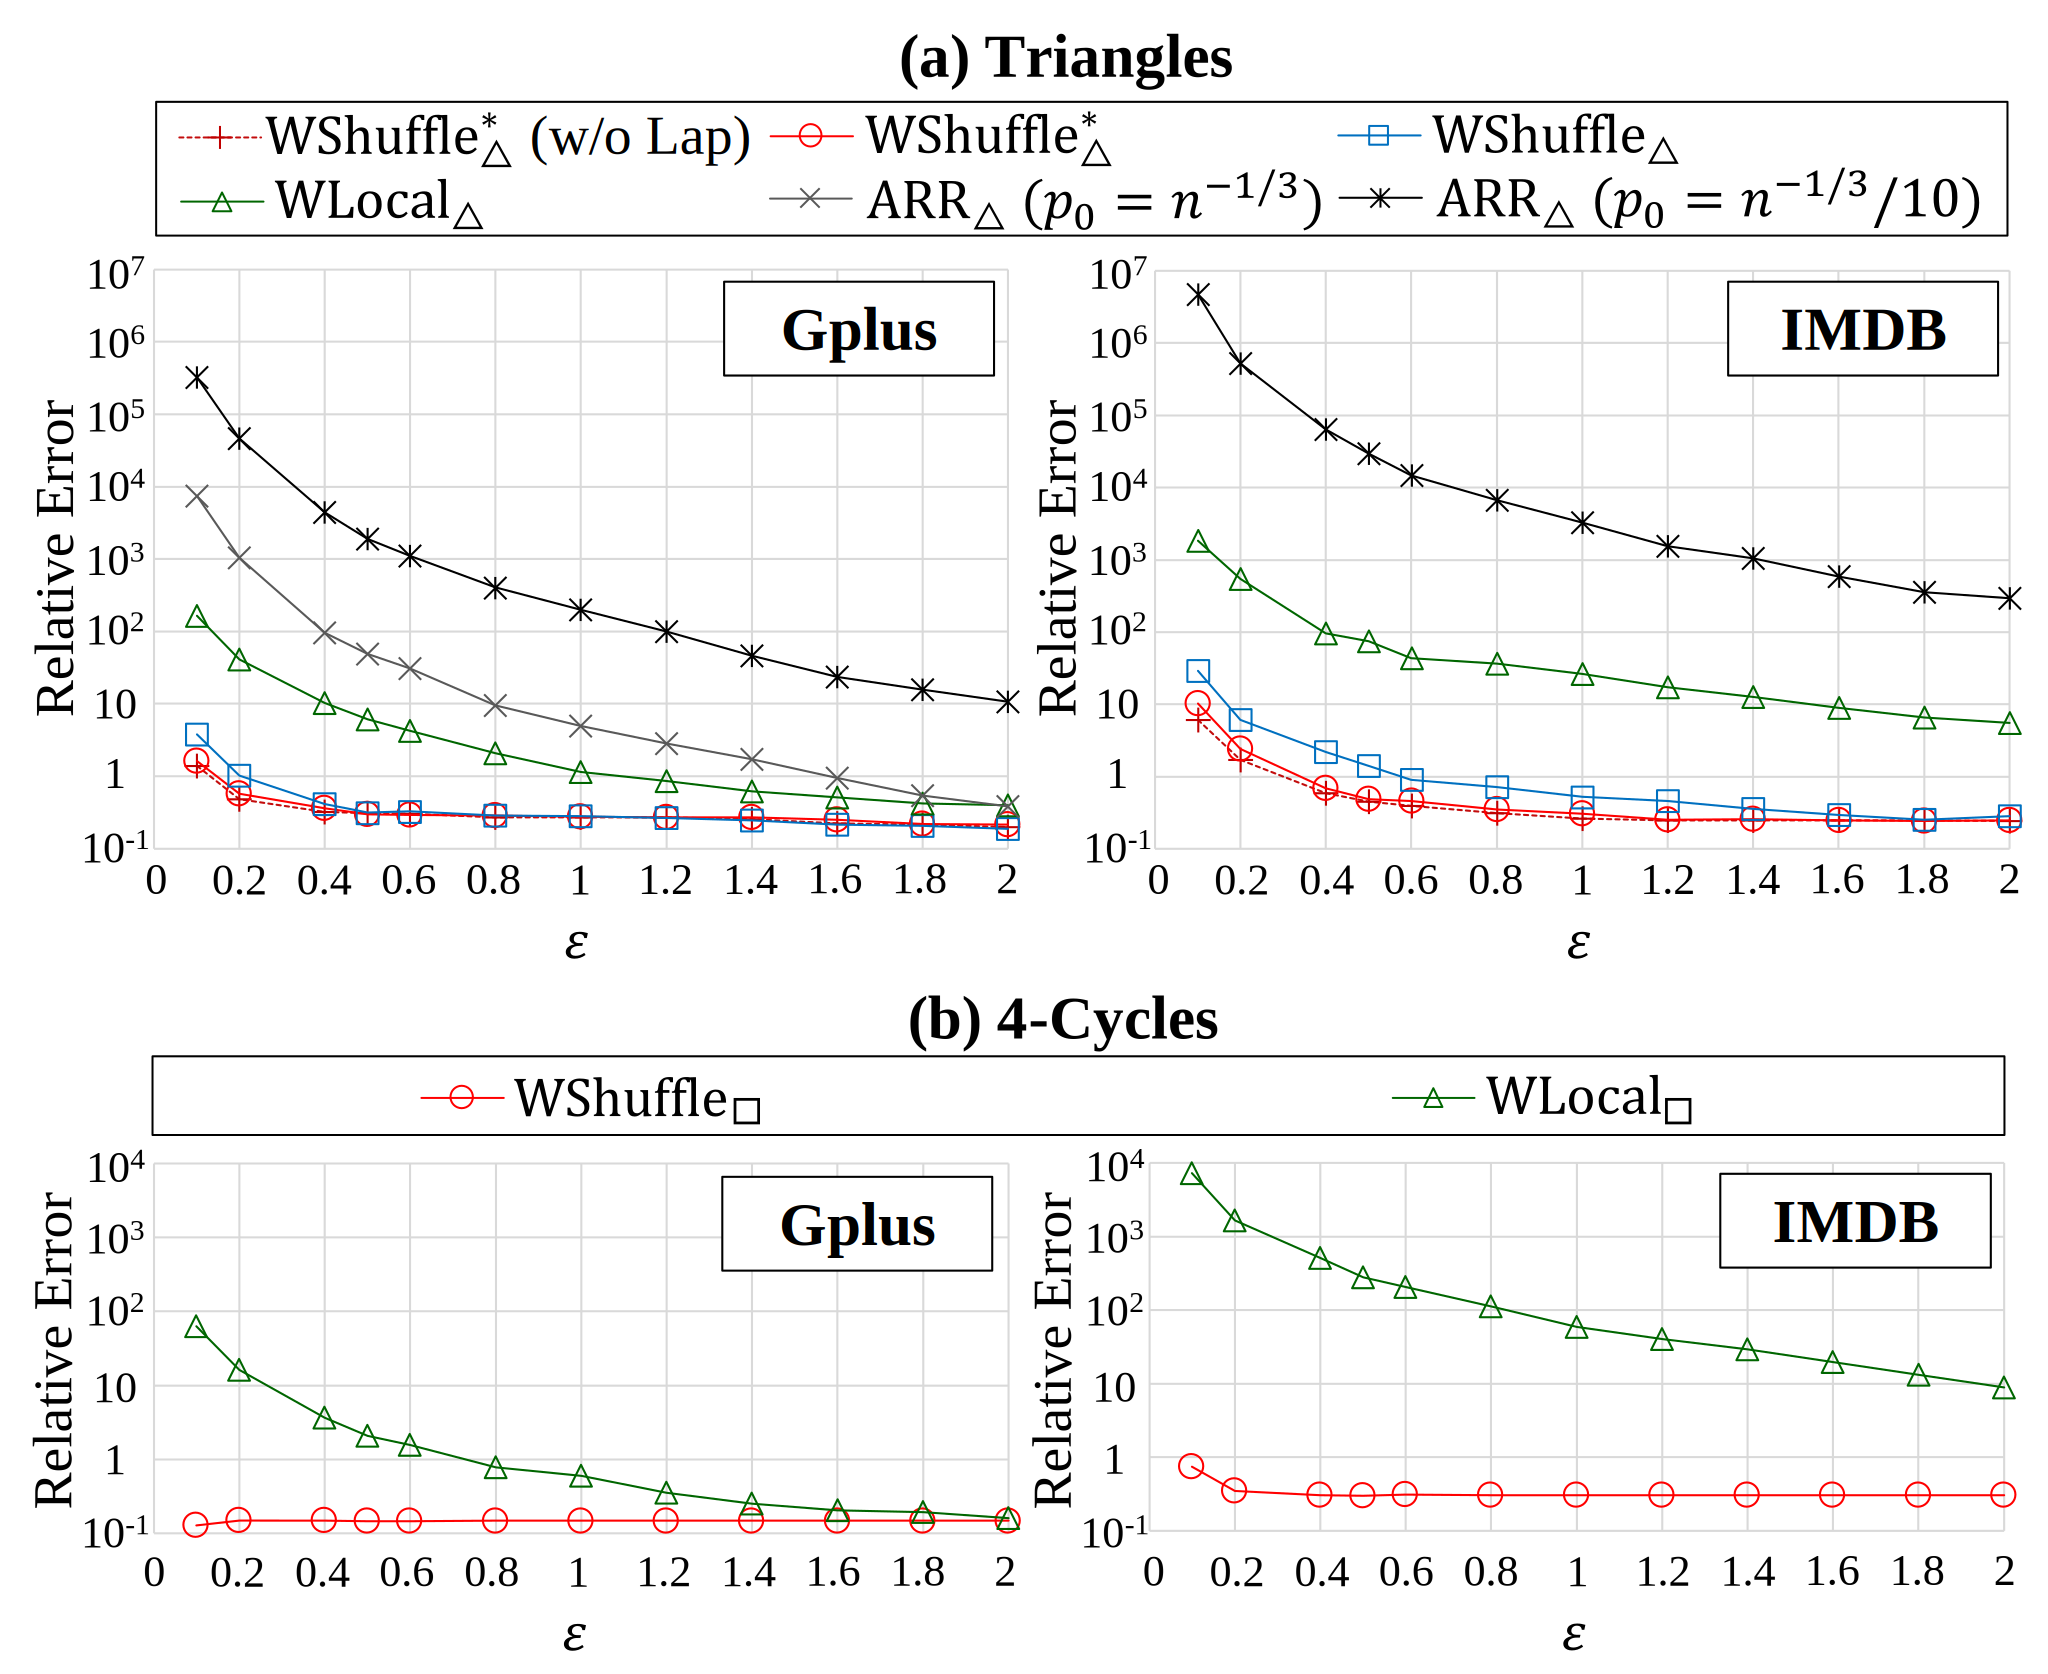
\includegraphics[width=0.99\linewidth]{fig/res1_eps.pdf}
  
  \caption{Relative error vs. $\epsilon$ 
  %in triangle counting 
  ($n=107614$ in \Gplus{}, $n=896308$ in \IMDB{}, $c=1$). 
  $p_0$ is the sampling probability in the ARR. 
  %; numerical bound in \cite{Feldman_FOCS21}). 
  }
  \label{chap3-fig:res1_eps}
\end{figure}

% \begin{table}[t]
%   \centering
%   (a) \Gplus{}\\
%   \begin{tabular}{|c|c|c|c|}
%     \hline
%     & \AlgWSTriVR{} & \AlgWSTri{} & \AlgWSCyc{} \\ \hline
%     $\epsilon=0.5$ & $0.298$ & $0.312$ & $0.145$ \\ \hline
%     $\epsilon=1$ & $0.277$ & $0.279$ & $0.147$ \\ \hline
%   \end{tabular}\\
%   (b) \IMDB{}\\
%   \begin{tabular}{|c|c|c|c|}
%     \hline
%      & \AlgWSTriVR{} & \AlgWSTri{} & \AlgWSCyc{} \\ \hline
%     $\epsilon=0.5$ & $0.488$ & $1.41$ & XX \\ \hline
%     $\epsilon=1$ & $0.308$ & $0.522$ & XX \\ \hline
%   \end{tabular}
%   \caption{Relative error when $\epsilon=0.5$ or $1$ ($n=107614$ in \Gplus{} and $896308$ in \IMDB{}; $c=1$). 
%   }
%   \label{chap3-tab:res1_eps_tri_0.5}
% \end{table}

\begin{table}[t]
  \caption{Relative error (RE) when $\epsilon=0.5$ or $1$ and computational time ($n=107614$ in \Gplus{}, $n=896308$ in \IMDB{}, $c=1$). 
  The lowest relative error is highlighted in bold.
  }
  
  \centering
%   (a) Triangle (\Gplus{})\\
  (a) \Gplus{}\\
  \begin{tabular}{|c|c|c|c|}
    \hline
    & RE ($\epsilon=0.5$) & RE ($\epsilon=1$) & Time (sec)\\ \hline
    \AlgWSTriVR{} & $\bm{2.98 \times 10^{-1}}$ & $\bm{2.77 \times 10^{-1}}$ & $3.60 \times 10^1$ \\ \hline
    \AlgWSTri{} & $3.12 \times 10^{-1}$ & $2.79 \times 10^{-1}$ & $3.62 \times 10^1$ \\ \hline
    \AlgWLTri{} & $6.10 \times 10^0$ & $1.14 \times 10^0$ & $5.83 \times 10^1$ \\ \hline
    \AlgARRTri{} ($p_0=n^{-1/3}$) & $4.90 \times 10^1$ & $4.93 \times 10^0$ & $7.15 \times 10^2$ \\ \hline
    \hspace{-0.5mm}\AlgARRTri{} ($p_0=0.1n^{-1/3}$)\hspace{-0.5mm} & $1.88 \times 10^3$ & $1.97 \times 10^2$ & $3.48 \times 10^1$ \\ \hline \hline
    \AlgWSCyc{} & $\bm{1.45 \times 10^{-1}}$ & $\bm{1.47 \times 10^{-1}}$ & $3.47 \times 10^1$ \\ \hline
    \AlgWLCyc{} & $2.08 \times 10^0$ & $5.96 \times 10^{-1}$ & $5.70 \times 10^1$ \\ \hline
  \end{tabular}\\
%   (b) Triangle (\IMDB{})\\
  (b) \IMDB{}\\
  \begin{tabular}{|c|c|c|c|}
    \hline
    & RE ($\epsilon=0.5$) & RE ($\epsilon=1$) & Time (sec)\\ \hline
    \AlgWSTriVR{} & $\bm{4.88 \times 10^{-1}}$ & $\bm{3.08 \times 10^{-1}}$ & $2.39 \times 10^3$ \\ \hline
    \AlgWSTri{} & $1.41 \times 10^0$ & $5.22 \times 10^{-1}$ & $2.40 \times 10^3$ \\ \hline
    \AlgWLTri{} & $7.46 \times 10^1$ & $2.63 \times 10^1$ & $3.96 \times 10^3$ \\ \hline
    \hspace{-0.5mm}\AlgARRTri{} ($p_0=0.1n^{-1/3}$)\hspace{-0.5mm} & $2.98 \times 10^4$ & $3.27 \times 10^3$ & $2.81 \times 10^3$ \\ \hline \hline
    \AlgWSCyc{} & $\bm{3.03 \times 10^{-1}}$ & $\bm{3.08 \times 10^{-1}}$ & $2.29 \times 10^3$ \\ \hline
    \AlgWLCyc{} & $2.82 \times 10^2$ & $5.91 \times 10^1$ & $3.91 \times 10^3$ \\ \hline
  \end{tabular}
%   (c) 4-cycle (\Gplus{})\\
%   \begin{tabular}{|c|c|c|c|}
%     \hline
%     & RE ($\epsilon=0.5$) & RE ($\epsilon=1$) & Time (sec)\\ \hline
%     \AlgWSCyc{} & $XXX$ & $XXX$ & $XXX$ \\ \hline
%     \AlgWLCyc{} & $XXX$ & $XXX$ & $XXX$ \\ \hline
%   \end{tabular}\\
  \label{chap3-tab:res1_eps_tri_time}
\end{table}

Figure~\ref{chap3-fig:res1_eps} shows the relative error ($c=1$). 
% Here, we used the numerical upper bound in \cite{Feldman_FOCS21} for $\epsilon$ in the shuffle algorithms. 
% We also 
Here, we show the performance of \AlgWSTri{} when we do not add the Laplacian noise (denoted by \AlgWSTri{} (w/o Lap)). 
In \IMDB{}, we do not show \AlgARRTri{} with $p_0 = n^{-1/3}$, because it takes too much time (longer than one day). 
Table~\ref{chap3-tab:res1_eps_tri_time} highlights the relative error when $\epsilon=0.5$ or $1$. 
It also shows the running time of counting triangles or 4-cycles when $\epsilon=1$ (we verified that the running time had little dependence on $\epsilon$). 

Figure~\ref{chap3-fig:res1_eps} and Table~\ref{chap3-tab:res1_eps_tri_time} show that our shuffle algorithms dramatically improve the local algorithms. 
% For example, 
In triangle counting, 
\AlgWSTriVR{} outperforms \AlgWLTri{} by one or two orders of magnitude and \AlgARRTri{} by even more\footnote{Note that \AlgARRTri{} uses only the lower-triangular part of the adjacency matrix $\bmA$ and therefore provides 
% $\epsilon$-edge LDP and 
$\epsilon$-edge DP (rather than $2\epsilon$-edge DP); i.e., it does not suffer from the doubling issue explained in Section~\ref{chap3-sub:privacy}. However, Figure~\ref{chap3-fig:res1_eps} shows that \AlgWSTriVR{} significantly outperforms \AlgARRTri{} 
% with the same privacy budget in edge DP.
even if we double $\epsilon$ for only \AlgWSTriVR{}.}. 
% Although the relative error of \AlgARRTri{} can be improved by using a larger $p_0$, it results in longer running time. 
\AlgWSTriVR{} also requires less running time than \AlgARRTri{} with $p_0 = n^{-1/3}$. 
Although the running time of \AlgARRTri{} can be improved by using a smaller $p_0$, it results in a higher relative error. 
% Similarly, 
In 4-cycle counting, 
\AlgWSCyc{} significantly outperforms \AlgWLCyc{}. 
The difference between our shuffle algorithms and the local algorithms is larger in \IMDB{} because it is more sparse; i.e., the difference between $d_{max}$ and $n$ is larger in \IMDB{}. 
This is consistent with our theoretical results in Tables~\ref{chap3-tab:upper_bounds_triangle} and \ref{chap3-tab:upper_bounds_4cycle}. 

Figure~\ref{chap3-fig:res1_eps} and Table~\ref{chap3-tab:res1_eps_tri_time} also show that \AlgWSTriVR{} outperforms \AlgWSTri{}, especially when $\epsilon$ is small. 
% or the dataset is sparse, i.e., \IMDB{}. 
This is because the variance is large when $\epsilon$ is small. 
In addition, \AlgWSTriVR{} significantly outperforms \AlgWSTri{} in \IMDB{} because \AlgWSTriVR{} significantly reduces the variance when $d_{max} \ll n$, as shown in Table~\ref{chap3-tab:upper_bounds_triangle}. 
In other words, this is also consistent with our theoretical results. 
For example, when $\epsilon=0.5$, our variance reduction technique reduces the relative error from $1.41$ to $0.488$ (about one-third) in \IMDB{}. 

Furthermore, Figure~\ref{chap3-fig:res1_eps} shows that the relative error of \AlgWSTriVR{} is hardly changed by adding the Laplacian noise. 
This is because the sensitivity of each user's degree $d_i$ is very small ($=1$). 
In this case, the Laplacian noise is also very small. 

\begin{figure}[t]
  \centering
  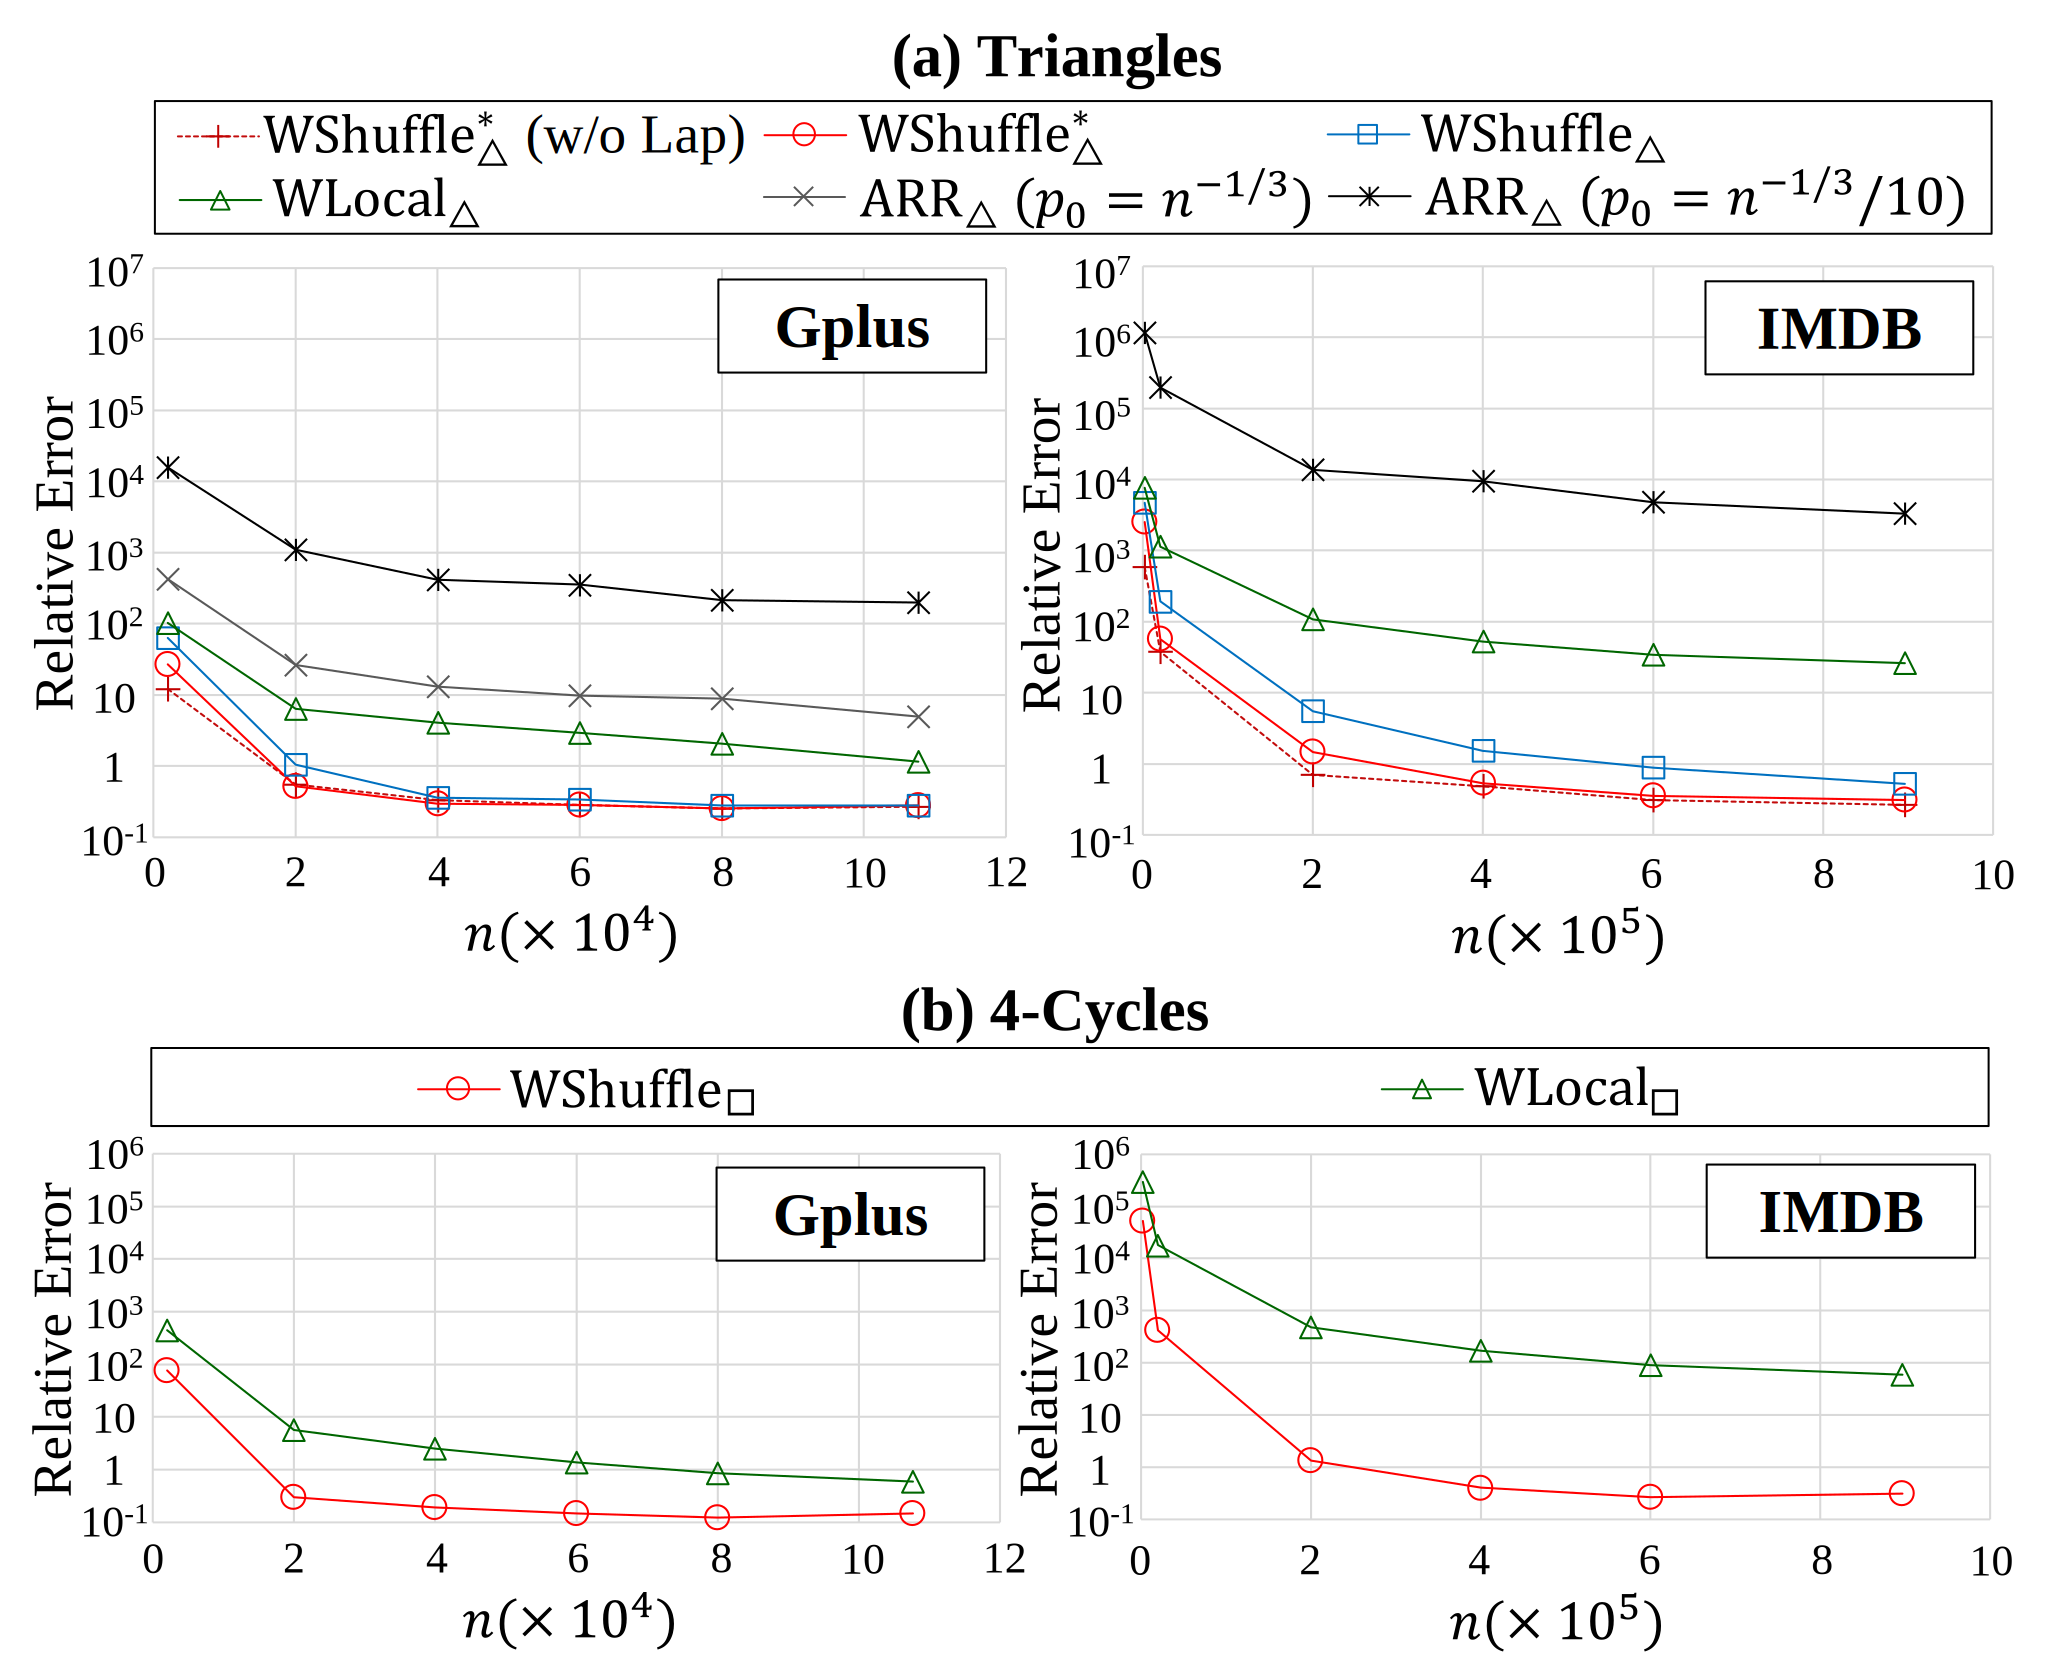
\includegraphics[width=0.99\linewidth]{fig/res2_n.pdf}
  
  \caption{Relative error vs. $n$ ($\epsilon=1$, $c=1$).
  }
  \label{chap3-fig:res2_n}
\end{figure}

% Table~\ref{chap3-tab:res1_eps_tri_time} shows that 
Our \AlgWSTriVR{} achieves a relative error of $0.3$ ($\ll 1$) 
% and \AlgWSCyc{} achieve relative errors of $0.15$ to $0.3$ ($\ll 1$) 
% with a reasonable privacy budget -- $\epsilon = 0.5$ or $1$ in element DP and $2\epsilon = 1$ or $2$ in edge DP. 
when the privacy budget is $\epsilon = 0.5$ or $1$ in element DP ($2\epsilon = 1$ or $2$ in edge DP). 
\AlgWSCyc{} achieve a relative error of $0.15$ to $0.3$ with a smaller privacy budget (e.g., $\epsilon = 0.2$) because it  does not send local edges -- the error of \AlgWSCyc{} is mainly caused by user-pair sampling that is independent of $\epsilon$. 

In summary, our \AlgWSTriVR{} and \AlgWSCyc{} significantly outperform the local algorithms and achieve a relative error much smaller than $1$ with a reasonable privacy budget, i.e., $\epsilon \leq 1$. 

\smallskip
\noindent{\textbf{Relative Error vs. $n$.}}~~Next, we evaluated the relation between the relative error and $n$. 
% the number $n$ of users. 
Specifically, we randomly selected $n$ users from all users and extracted a graph with $n$ users. 
Then we set $\epsilon = 1$ and changed $n$ to various values starting from $2000$. 
%from $2000$ to $107614$ and $896308$ in \Gplus{} and \IMDB{}, respectively. 

Figure~\ref{chap3-fig:res2_n} shows the results ($c=1$). 
% We observe that 
When $n=2000$, \AlgWSTri{} and \AlgWSCyc{} provide 
%almost the same relative error as 
relative errors close to \AlgWLTri{} and \AlgWLCyc{}, respectively. 
This is because the privacy amplification effect is limited when $n$ is small. 
For example, when $n=2000$ and $\epsilon=1$, 
% and $\delta=10^{-8}$, 
the numerical bound is $\epsilon_L=1.88$. 
The value of $\epsilon_L$ increases with increase in $n$; e.g., when $n=107614$ and $896308$, the numerical bound is $\epsilon_L= 5.86$ and $7.98$, respectively. 
This explains the reason that our shuffle algorithms significantly outperform the local algorithms when $n$ is large in Figure~\ref{chap3-fig:res2_n}. 
% the large difference between our shuffle algorithms and the local algorithms. 
% in Figure~XX. 

% Figure~XX also shows that the relative error decreases with increase in $n$. 
% There are two reasons for this: (i) the squares of the true triangle and 4-cycle counts are $O(n^2 d_{max}^4)$ and $O(n^2 d_{max}^6)$, respectively; (ii) $d_{max}$ is proportional to $n$, as we randomly selected $n$ users from all users. 


% \smallskip
% \noindent{\textbf{Clustering Coefficient.}}~~TBD

\smallskip
\noindent{\textbf{Parameter $c$ in \AlgWSTriVR{}.}}~~Finally, we evaluated our \AlgWSTriVR{} while changing the parameter $c$ that controls the bias and variance. 
% of the estimate. 
Recall that as $c$ increases, the bias is increased, and the variance is reduced. 
We set $\epsilon=0.1$ or $1$ and changed $c$ from $0.1$ to $4$. 

Figure~\ref{chap3-fig:res4_thr} shows the results. 
Here, we also show the relative error of \AlgWSTri{}. 
We observe that the optimal $c$ is different for $\epsilon=0.1$ and $\epsilon=1$. The optimal $c$ is around $3$ to $4$ for $\epsilon=0.1$, whereas the optimal $c$ is around $0.5$ to $1$ for $\epsilon=1$. 
This is because the variance of \AlgWSTri{} is large (resp.~small) when $\epsilon$ is small (resp.~large). 
For a small $\epsilon$, a large $c$ is effective in significantly reducing the variance. 
For a large $\epsilon$, a small $c$ is effective in keeping a small bias. 
% The optimization of $c$ in \AlgWSTriVR{} is an interesting future research direction. 

We also observe that \AlgWSTriVR{} is always better than (or almost the same as) \AlgWSTri{} when $c=1$ or $2$. 
This is because most users' degrees are smaller than the average degree $d_{avg}$, as described in Section~\ref{chap3-sub:var_red}. 
When $c=1$ or $2$, most user-pairs are ignored. 
Therefore, we can significantly reduce the variance at the cost of a small bias. 

\begin{figure}[t]
  \centering
  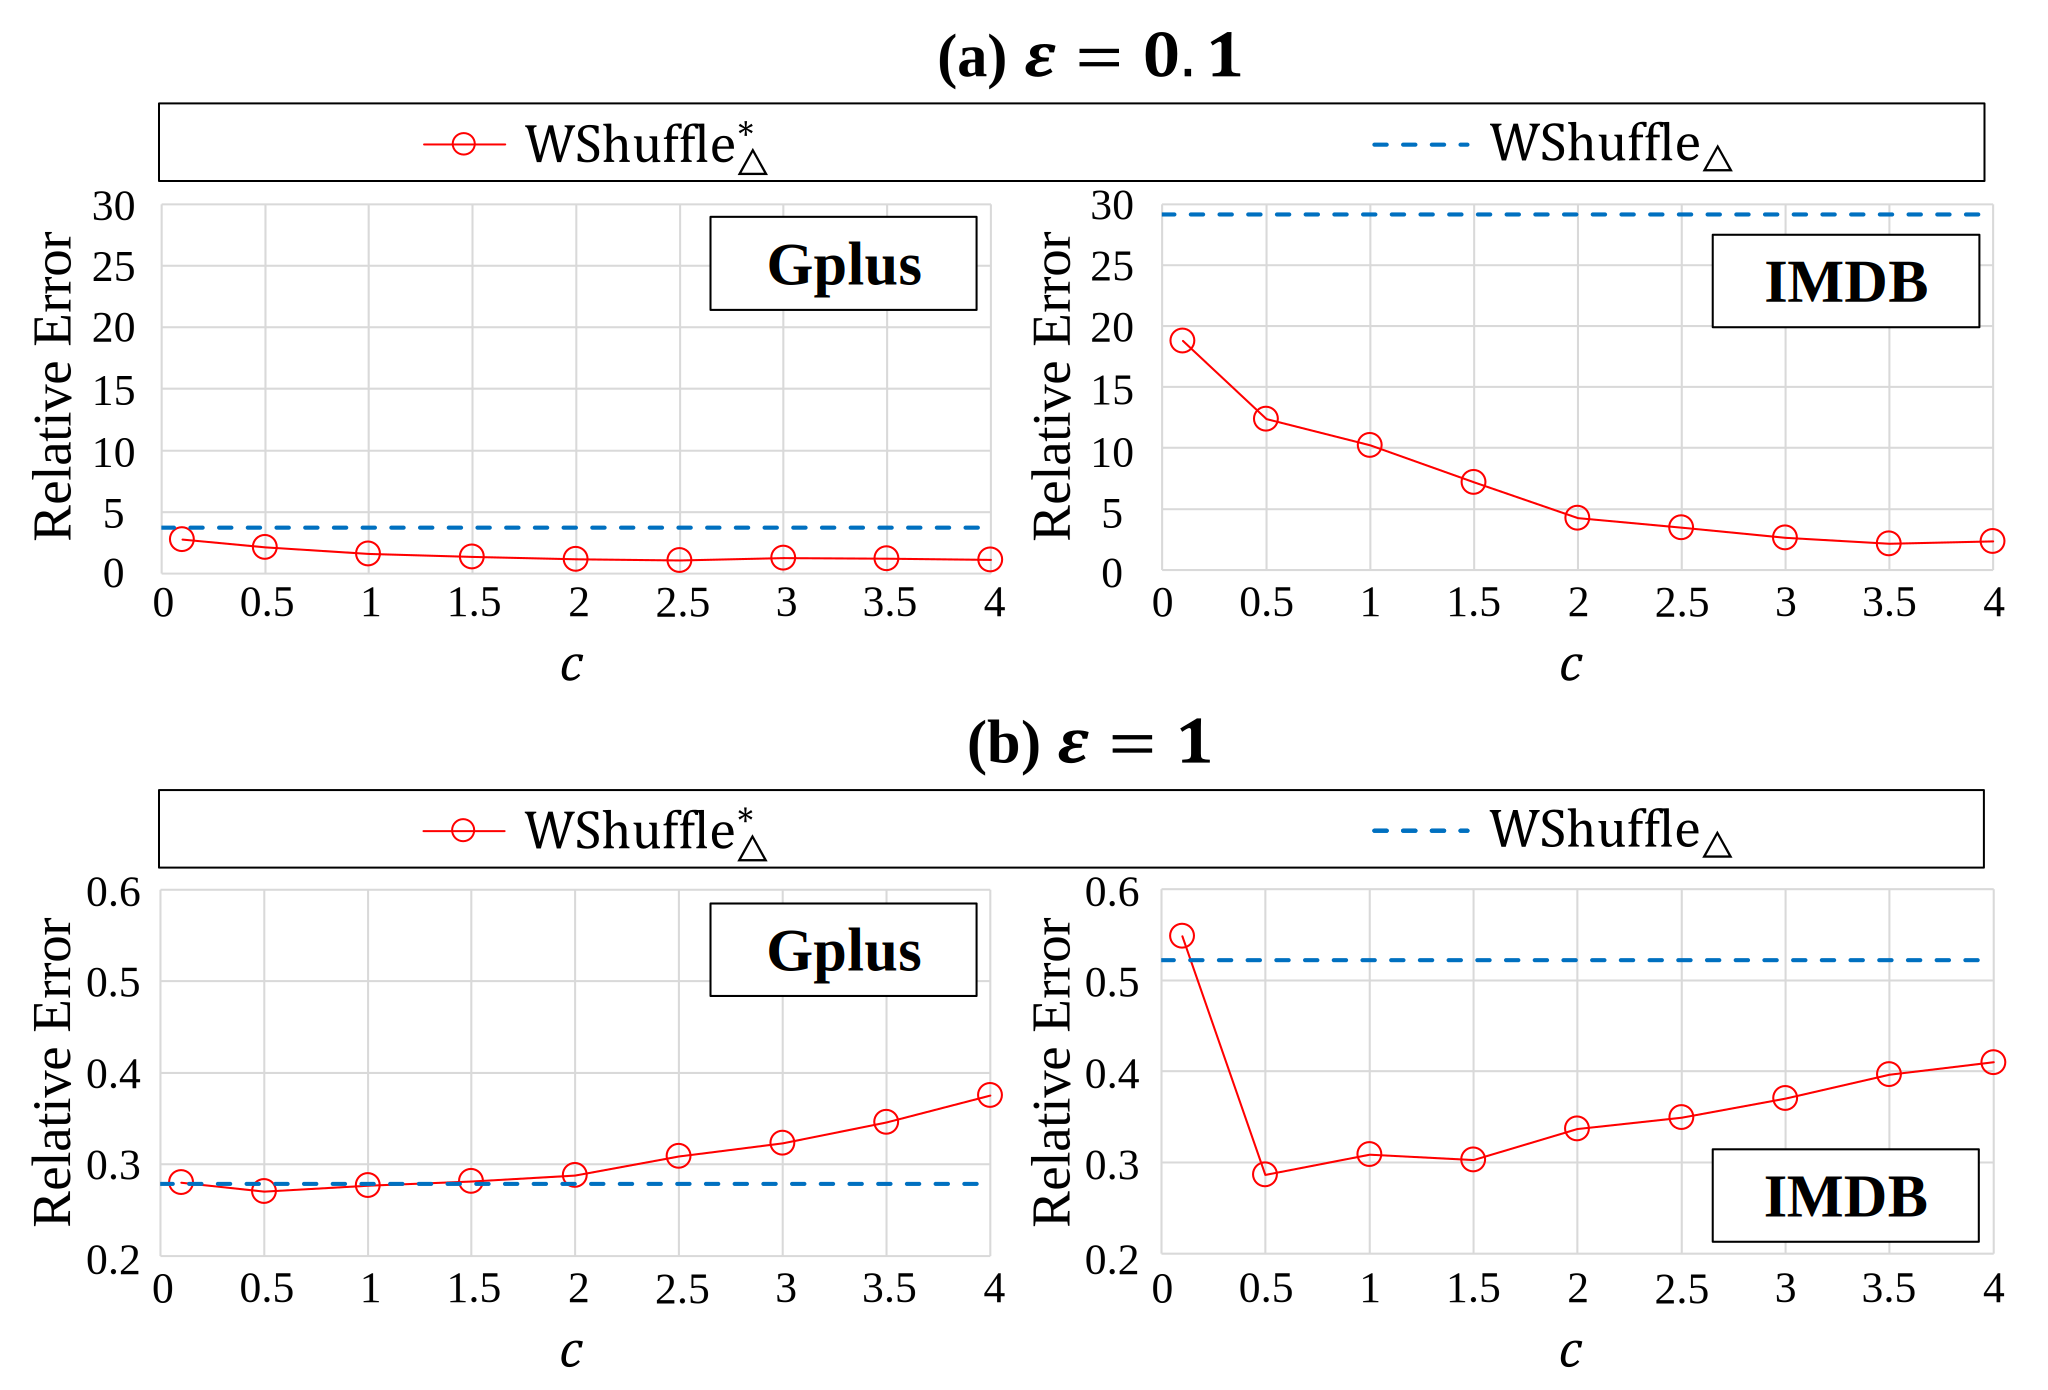
\includegraphics[width=0.99\linewidth]{fig/res4_thr.pdf}
  
  \caption{Relative error vs. parameter $c$ in \AlgWSTriVR{} ($n=107614$ in \Gplus{}, $n=896308$ in \IMDB{}).
  }
  \label{chap3-fig:res4_thr}
\end{figure}

\smallskip
\noindent{\textbf{Summary.}}~~In summary, our answers to the three questions at the beginning of Section~\ref{chap3-sec:experiments} are as follows. 
RQ1: Our \AlgWSTriVR{} and \AlgWSCyc{} outperform the one-round local algorithms by one or two orders of magnitude (or even more). 
% \AlgWSTriVR{} is even comparable to the two-rounds local algorithm in \cite{Imola_USENIX22} (\AlgTwoRS{}) that requires a lot of user effort 
% and synchronization 
% in terms of accuracy. 
RQ2: Our variance reduction technique significantly reduces the relative error (e.g., by about one-third) 
for a small $\epsilon$ in a sparse dataset. 
% when $\epsilon$ is small or the dataset is sparse. 
RQ3: 
% Our \AlgWSTriVR{} and \AlgWSCyc{} achieve a relative error of $0.15$ to $0.3$ ($\ll 1$) when $\epsilon=0.5$ or $1$ in element DP ($2\epsilon=1$ or $2$ in edge DP). 
\AlgWSTriVR{} achieves a relative error of $0.3$ ($\ll 1$) when $\epsilon=0.5$ or $1$ in element DP ($2\epsilon=1$ or $2$ in edge DP). 
\AlgWSCyc{} achieves a relative error of $0.15$ to $0.3$ with a smaller privacy budget: $\epsilon=0.2$. 

\section{Conclusion}
\label{sec:conclusion}
In this paper, we made the first attempt (to our knowledge) to 
shuffle graph data for privacy amplification. 
% apply the shuffle model to graph data. 
We proposed wedge shuffling as a basic technique and then applied it to 
% to enable the privacy amplification of graph data. 
% Then we proposed 
one-round triangle and 4-cycle counting with several additional techniques. 
% algorithms based on wedge shuffling. 
We showed upper bounds on 
% the expected $l_2$ loss 
the MSE 
for each algorithm. 
We also showed through comprehensive experiments that our one-round shuffle algorithms significantly outperform the one-round local algorithms and achieve a small relative error with a reasonable privacy budget, e.g., smaller than $1$ in edge DP. 

For future work, we would like to apply wedge shuffling to other subgraphs such as 3-hop paths \cite{Sun_CCS19} and $k$-triangles \cite{Karwa_PVLDB11}. 

%%
%% The acknowledgments section is defined using the "acks" environment
%% (and NOT an unnumbered section). This ensures the proper
%% identification of the section in the article metadata, and the
%% consistent spelling of the heading.
%\section*{Acknowledgments}
\begin{acks}
Kamalika Chaudhuri and Jacob Imola would like to thank ONR under N00014-20-1-2334 and UC Lab Fees under LFR 18-548554  for research support.
Takao Murakami was supported in part by JSPS KAKENHI JP22H00521 and JP19H01109.
\end{acks}

%%
%% The next two lines define the bibliography style to be used, and
%% the bibliography file.
\bibliographystyle{ACM-Reference-Format}
\bibliography{main}

%%
%% If your work has an appendix, this is the place to put it.
% \appendix
% \graphicspath{{./chapters/chapter2/}}
\chapter{ }

\section{Basic Notations}
\label{chap2-sec:notations_subgraphs}

Table~\ref{chap2-tab:notations} shows the basic notations used in this paper.
% We also show subgraphs that appear in our theoretical analysis (Theorem~\ref{chap2-thm:l2loss_algorithms}) in Figure~\ref{chap2-fig:subgraphs}.

\begin{table}[t]
\caption{Basic notations.}
\centering
\hbox to\hsize{\hfil
\begin{tabular}{l|l}
\hline
Symbol		&	Description\\
\hline
% $n$         &	    Number of users.\\
$G=(V,E)$   &	    Graph with $n$ users $V$ and edges $E$.\\
$v_i$       &       $i$-th user in $V$ (i.e., $V=\{v_1,\ldots,v_n\}$).\\
$d_{max}$   &       Maximum degree of $G$.\\
$\calG$     &       Set of possible graphs with $n$ users.\\
$f_\triangle(G)$   &  Triangle count in $G$.\\
$\bmA=(a_{i,j})$	    &		Adjacency matrix.\\
$\bma_i$	&		Neighbor list of $v_i$ (i.e., $i$-th row of $\bmA$).\\
% $\calR_i$     &       Randomized mechanism of $v_i$.\\
$\calR_i$     &       Local randomizer of $v_i$.\\
$M_i$     &       Message sent from the server to user $v_i$.\\
% $\mu_F$     &       ARR parameter $\mu$ in \AlgOne{}.\\
% $\mu_O$     &       ARR parameter $\mu$ in \AlgTwo{}.\\
% $\mu_T$     &       ARR parameter $\mu$ in \AlgThree{}.\\
$\mu$     &       Parameter in the ARR.\\
$\mu^*$     &   $=\mu, \mu^2, \mu^3$ in \AlgOne{}, \AlgTwo{}, \\
    &   and \AlgThree{}, respectively.\\
$\td_i$     &   Noisy degree of user $v_i$.\\
$\kappa_i$ &   Clipping threshold of user $v_i$.\\
% $\lambda_i$ &   Clipping coefficient of user $v_i$.\\
$\epsilon_0$     &       Privacy budget for edge clipping.\\
$\epsilon_1$     &       Privacy budget for the ARR.\\
$\epsilon_2$     &       Privacy budget for the Laplacian noise.\\
$\epsilon$     &       Total privacy budget.\\
\hline
\end{tabular}
\hfil}
\label{chap2-tab:notations}
\end{table}

\section{Comparison with One-Round Algorithms}
\label{chap2-sec:one-round}
% Some studies \cite{Imola_USENIX21,Ye_ICDE20,Ye_TKDE21} propose one-round triangle counting algorithms.

Below we show that one-round triangle counting algorithms suffer from a prohibitively large estimation error.

First, we note that all of the existing one-round triangle algorithms in \cite{Imola_USENIX21,Ye_ICDE20,Ye_TKDE21} are inefficient and \textit{cannot be directly applied to a large-scale graph} such as \GPlus{} and \IMDB{} in Section~\ref{chap2-sec:experiments}.
Specifically, in their algorithms, each user $v_i$ applies Warner's RR to each bit of her neighbor list $\bma_i$ and sends the noisy neighbor list to the server.
Then the server counts the number of noisy triangles, each of which has three noisy edges,
% from the noisy graph $G'$,
and estimates $f_\triangle(G)$ based on the noisy triangle count. 
The noisy graph $G'$ in the server is dense, and there are $O(n^3)$ noisy triangles in $G'$. 
Thus, the time complexity of the existing one-round algorithms \cite{Imola_USENIX21,Ye_ICDE20,Ye_TKDE21} is $O(n^3)$.
It is also reported in \cite{Imola_USENIX21} that when $n=10^6$, the one-round algorithms  would require about $35$ years even using a supercomputer, due to the enormous number of noisy triangles.

Therefore, we evaluated the existing one-round algorithms by taking the following two steps.
First, we evaluate all the existing algorithms in \cite{Imola_USENIX21,Ye_ICDE20,Ye_TKDE21} using small graph datasets ($n=10000$) and show that the algorithm in \cite{Imola_USENIX21} achieves the lowest estimation error.
Second, we improve the time complexity of the algorithm in \cite{Imola_USENIX21} using the ARR (i.e., edge sampling after Warner's RR) and compare it with our two-rounds algorithms using large graph datasets in Section~\ref{chap2-sec:experiments}.

\smallskip
\noindent{\textbf{Small Datasets.}}~~We first evaluated the existing algorithms in \cite{Imola_USENIX21,Ye_ICDE20,Ye_TKDE21} using small datasets.
For both \GPlus{} and \IMDB{} in Section~\ref{chap2-sec:experiments}, we first randomly selected $n=10000$ users from all users and extracted a graph with $n$ users.
Then we evaluated the relative error of the following three algorithms:
(i) \textsf{RR (biased)} \cite{Imola_USENIX21,Ye_ICDE20},
(ii) \textsf{RR (bias-reduced)} \cite{Ye_TKDE21}, and
(iii) \textsf{RR (unbiased)} \cite{Imola_USENIX21}.
All of them provide $\epsilon$-edge LDP.

% The first algorithm
\textsf{RR (biased)} simply uses the number of noisy triangles in the noisy graph $G'$ obtained by Warner's RR
% each of which has three edges
as an estimate of $f_\triangle(G)$.
Clearly, it suffers from a very large bias, as $G'$ is dense.
% The second algorithm
\textsf{RR (bias-reduced)} reduces
% the bias of \textsf{RR (biased)}
this bias
by using a noisy degree sent by each user.
However, it introduces some approximation to estimate $f_\triangle(G)$, and consequently, it is not clear whether the estimate is unbiased.
We used the mean of the noisy degrees as a representative degree to obtain the optimal privacy budget allocation (see \cite{Ye_TKDE21} for details).
% The third algorithm
\textsf{RR (unbiased)} calculates an unbiased estimate of $f_\triangle(G)$ via empirical estimation. It is proved that the estimate is unbiased \cite{Imola_USENIX21}.

In all of the three algorithms, each user $v_i$ obfuscates bits for smaller user IDs in her neighbor list $\bma_i$. 
% (i.e., the lower triangular part of $\bmA$) 
% to avoid the doubling issue in Section~\ref{chap2-sub:LDP}.
We averaged the relative error over $10$ runs.

\begin{figure}[t]
  \centering
  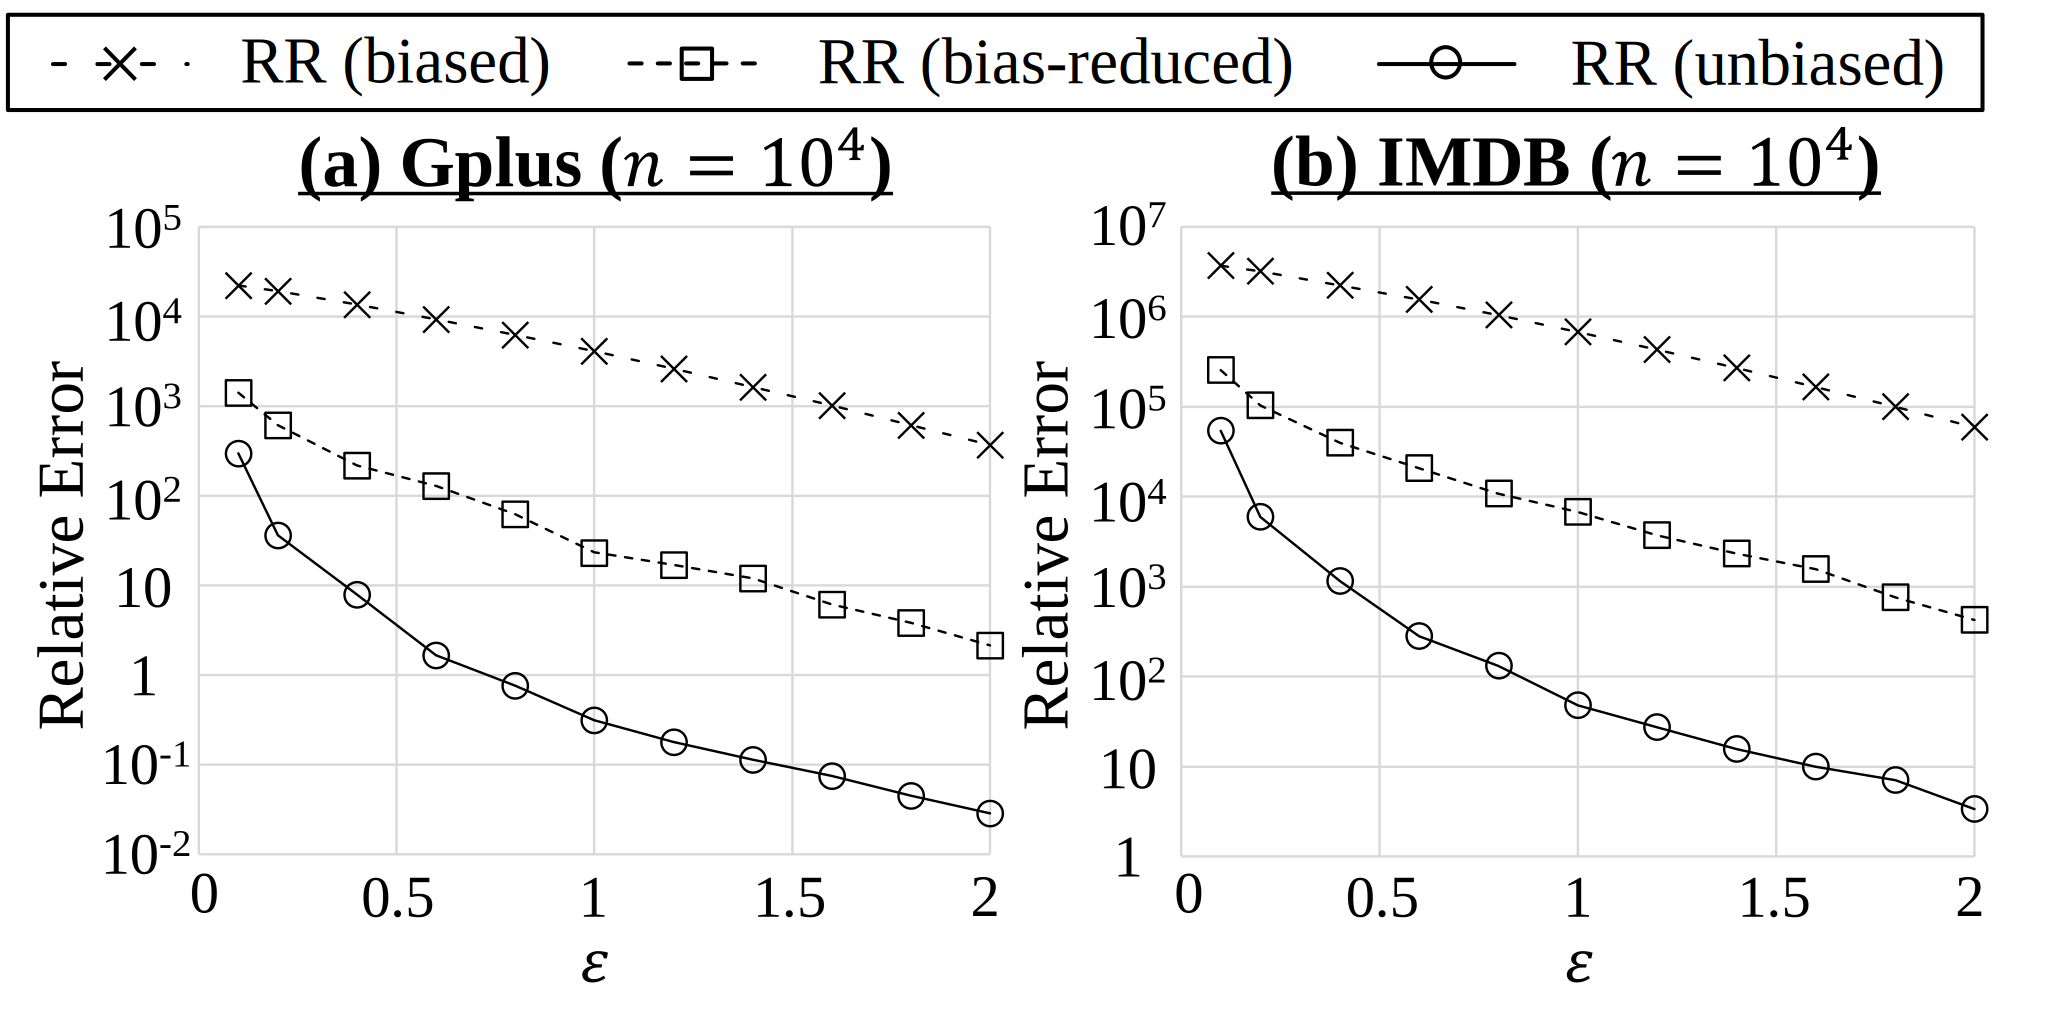
\includegraphics[width=0.99\linewidth]{fig/resB_one_round_small.pdf}
  
  \caption{Relative error of one-round algorithms for small datasets ($n=10000$).}
  \label{chap2-fig:resB_small}
\end{figure}

Figure~\ref{chap2-fig:resB_small} shows the results.
\textsf{RR (bias-reduced)} significantly outperforms \textsf{RR (biased)} and is significantly outperformed by \textsf{RR (unbiased)}.
We believe 
% that 
this is caused by the fact that \textsf{RR (bias-reduced)} introduces some approximation and does not calculate an unbiased estimate of $f_\triangle(G)$.

\smallskip
\noindent{\textbf{Large Datasets.}}~~Based on Figure~\ref{chap2-fig:resB_small}, we improve the time complexity of \textsf{RR (unbiased)} using the ARR and compare it with our two-rounds algorithms in large datasets.

Specifically, \textsf{RR (unbiased)} counts \textit{triangles}, \textit{$2$-edges} (three nodes with two edges), \textit{$1$-edges} (three nodes with one edge), and \textit{no-edges} (three nodes with no edges) in $G'$ obtained by Warner's RR.
Let $m_3, m_2, m_1, m_0 \in \nnints$ be the numbers of triangles, $2$-edges, $1$-edges, and no-edges, respectively, after applying Warner's RR.
\textsf{RR (unbiased)} calculates an unbiased estimate of $f_\triangle(G)$ from these four values.
Thus, we improve \textsf{RR (unbiased)} by using the ARR, which samples each edge with probability $p_2$ after Warner's RR, and then calculating unbiased estimates of $m_3$, $m_2$, $m_1$, and $m_0$.

Let $\hat{m}_3, \hat{m}_2, \hat{m}_1, \hat{m}_0 \in \reals$ be the unbiased estimates of $m_3$, $m_2$, $m_1$, and $m_0$, respectively. 
% after applying Warner's RR.
Let $m_3^*, m_2^*, m_1^*, m_0^* \in \nnints$ be the number of triangles, 2-edges, 1-edges, no-edges, respectively, after applying the ARR.
Since the ARR samples each edge with probability $p_2$, we obtain:
\begin{align*}
    m_3^* &= \textstyle{p_2^3 \hat{m}_3} \\
    m_2^* &= \textstyle{3p_2^2(1-p_2) \hat{m}_3 + p_2^2 \hat{m}_2} \\
    m_1^* &= \textstyle{3p_2(1-p_2)^2 \hat{m}_3 + 2p_2(1-p_2) \hat{m}_2 + p_2 \hat{m}_1.}
\end{align*}
By these equations,
% and $\hat{m}_3 + \hat{m}_2 + \hat{m}_1 + \hat{m}_0 = \frac{n(n-1)(n-2)}{6}$,
we obtain:
\begin{align}
    \hat{m}_3 &= \textstyle{\frac{m_3^*}{p_2^3}} \label{chap2-eq:hm_3} \\
    \hat{m}_2 &= \textstyle{\frac{m_2^*}{p_2^2} - 3(1-p_2)\hat{m}_3} \label{chap2-eq:hm_2} \\
    \hat{m}_1 &= \textstyle{\frac{m_1^*}{p_2} - 3(1-p_2)^2\hat{m}_3 - 2(1-p_2)\hat{m}_2} \label{chap2-eq:hm_1} \\
    \hat{m}_0 &= \textstyle{\frac{n(n-1)(n-2)}{6} - \hat{m}_3 - \hat{m}_2 - \hat{m}_1.} \label{chap2-eq:hm_0}
\end{align}
Therefore, after applying the ARR to the lower triangular part of $\bmA$, the server counts $m_3^*$, $m_2^*$, $m_1^*$, and $m_0^*$ in $G'$, and then calculates the unbiased estimates $\hat{m}_3$, $\hat{m}_2$, $\hat{m}_1$, and $\hat{m}_0$ by (\ref{chap2-eq:hm_3}), (\ref{chap2-eq:hm_2}), (\ref{chap2-eq:hm_1}), and (\ref{chap2-eq:hm_0}), respectively.
Finally, the server estimates $f_\triangle(G)$ from $\hat{m}_3$, $\hat{m}_2$, $\hat{m}_1$, and $\hat{m}_0$ in the same way as \textsf{RR (unbiased)}.
We denote this algorithm by \textsf{ARR (unbiased)}.
The time complexity of \textsf{ARR (unbiased)} is $O(\mu^3 n^3)$, where $\mu$ is the ARR parameter.

We compared \textsf{ARR (unbiased)} with our three algorithms with double clipping using \GPlus{} ($n=107614$) and \IMDB{} ($n=896308$).
For the sampling probability $p_2$, we set $p_2 = 10^{-3}$ or $10^{-6}$.
We averaged the relative error over $10$ runs.

\begin{figure}[t]
  \centering
  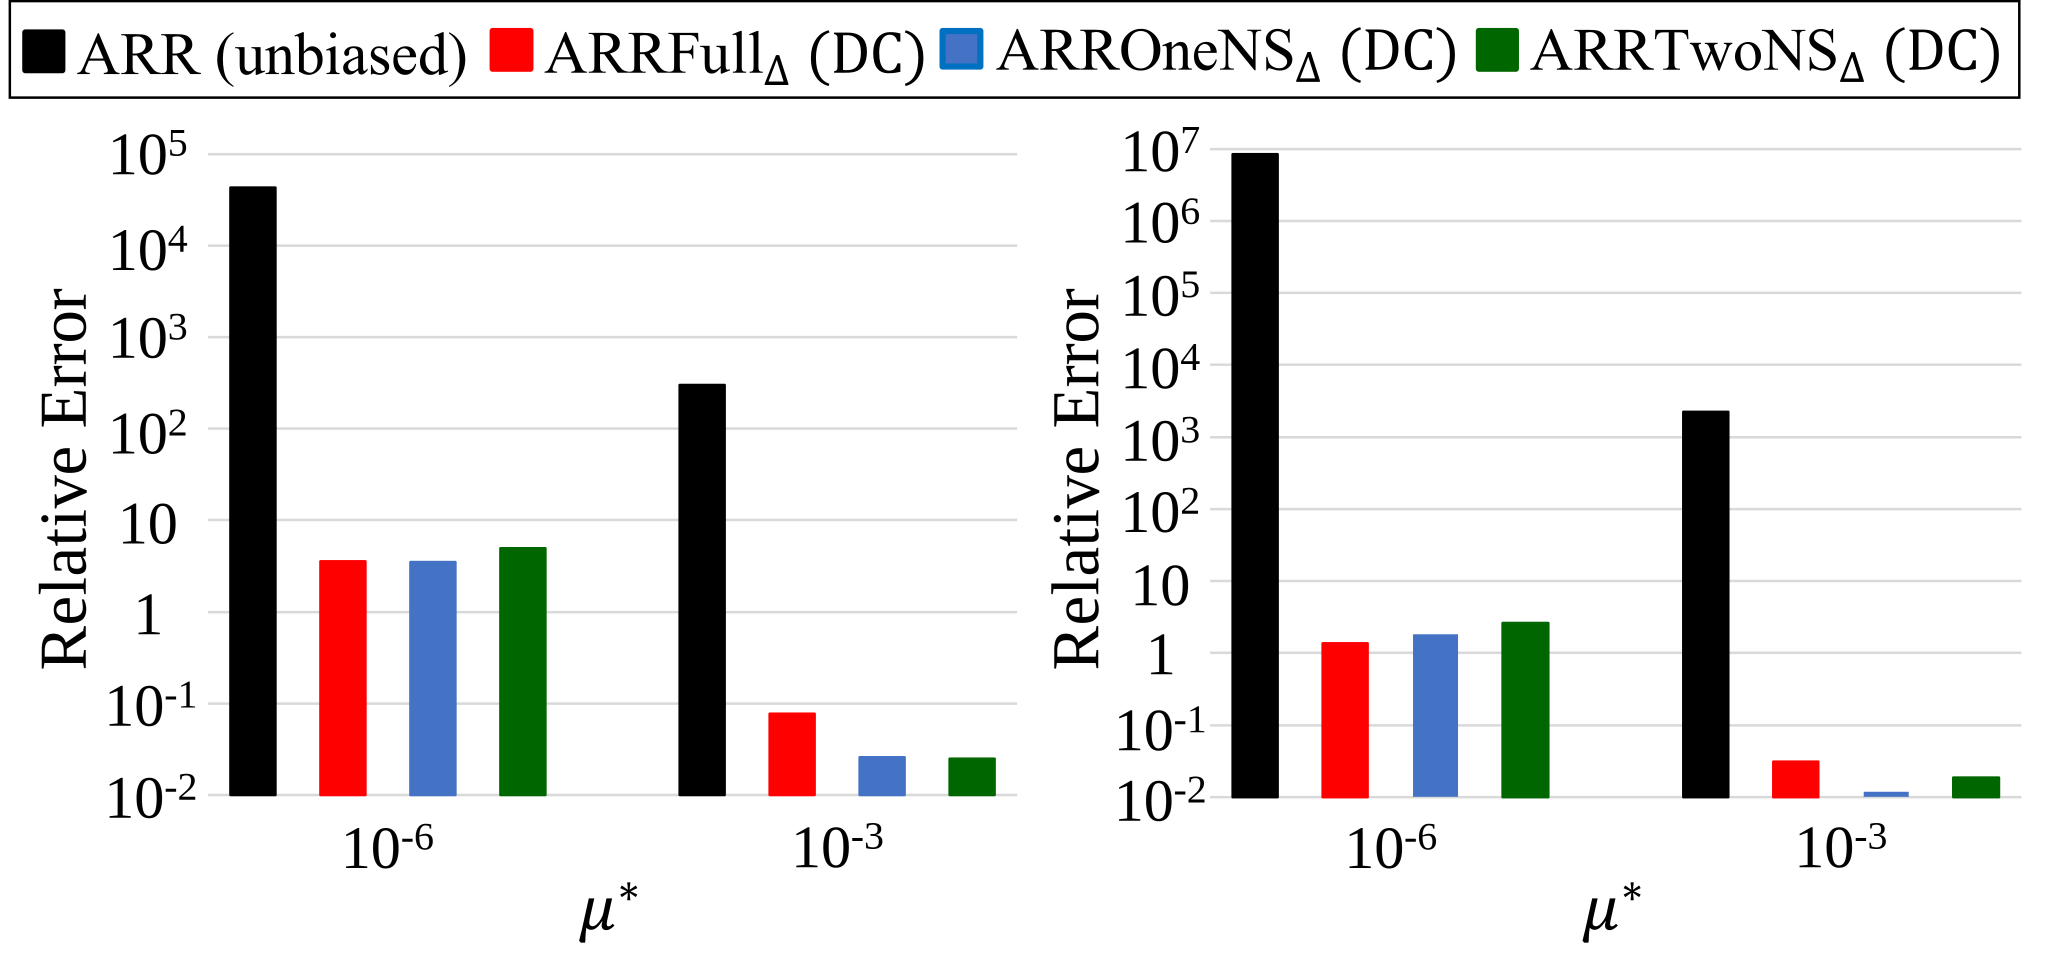
\includegraphics[width=0.99\linewidth]{fig/resB_one_round_large.pdf}
  
  \caption{Relative error of the one-round algorithm \textsf{ARR (unbiased)} and our three two-rounds algorithms with double clipping for large datasets ($n=107614$ in \GPlus{}, $n=896308$ in \IMDB{}).}
  \label{chap2-fig:resB_large}
\end{figure}

Figure~\ref{chap2-fig:resB_large} shows the results, where we set
% $\mu_F$ ($=\mu_o^2=\mu_T^3$)
$\mu^* = 10^{-6}$ or $10^{-3}$.
In \textsf{ARR (unbiased)}, we used $\mu^*$ as 
% a parameter $\mu$ of the ARR.
the ARR parameter $\mu$. 
Thus, we can see \textit{how much the relative error is reduced by introducing an additional round with \AlgOne{}}.
Figure~\ref{chap2-fig:resB_large} shows that the relative error of \textsf{ARR (unbiased)} is prohibitively large; i.e., relative error $\gg 1$.
% even when $\mu_F = 10^{-3}$.
This is because three edges are noisy in any noisy triangle. 
% and edge sampling is introduced to reduce the time complexity. 
% (recall that the one-round algorithms without sampling would require about $35$ years when $n=10^6$ \cite{Imola_USENIX21}).
% The relative error is extremely large when $\mu_F = 10^{-6}$ due to a very small sampling probability.
The relative error is significantly reduced by  introducing an additional round
% and counting noisy triangles in which only one edge is noisy.
% In contrast, our algorithms achieve much smaller estimation error
because only one edge is noisy in each noisy triangle at the second round.

In summary, one-round algorithms are far from acceptable in terms of the estimation error for large graphs, and two-round algorithms such as ours are necessary.

\section{Clustering Coefficient}
\label{chap2-sec:cluster}
% \smallskip
% \noindent{\textbf{Clustering Coefficient.}}~~We
Here we
% We have so far evaluated the estimation error of the triangle count.
% finally
% show that our algorithms are very useful for estimating the clustering coefficient.
evaluate the estimation error of the clustering coefficient using our algorithms.

% evaluated the estimation error of the clustering coefficient as follows.
We first estimated a triangle count by using our \AlgTwo{} with double clipping
($\epsilon_0 = \frac{\epsilon}{10}$ and
$\epsilon_1 = \epsilon_2 = \frac{9\epsilon}{20}$)
because it provides the best performance in Figures~\ref{chap2-fig:res2_w_Lap_abst}, \ref{chap2-fig:res2_w_Lap}, and \ref{chap2-fig:res3_n}.
Then we estimated a $2$-star count by
% a modified version of the algorithm in~\cite{Imola_USENIX21} using the adaptive edge clipping in Section~\ref{chap2-sec:double_clip}.
using the one-round $2$-star algorithm in~\cite{Imola_USENIX21} with the
% adaptive
edge clipping in Section~\ref{chap2-sec:double_clip}.

Specifically, we calculated a noisy degree $\td_i$ of each user $v_i$ 
% (possibly with edge clipping) 
by using the edge clipping with the privacy budget $\epsilon_0$.
Then we calculated the number $r_i \in \nnints$ of $2$-stars of which user $v_i$ is a center, and added $\Lap(\frac{\Delta}{\epsilon_1})$ to $r_i$, where $\Delta = \binom{\td_i}{2}$.
Let $\hr_i = r_i + \Lap(\frac{\Delta}{\epsilon_1})$ be the noisy $2$-star of $v_i$.
Finally, we calculated
% the sum of the noisy $2$-stars
the sum $\sum_{i=1}^n \hr_i$ as an estimate of the $2$-star count.
This $2$-star algorithm provides ($\epsilon_0 + \epsilon_1$)-edge privacy (see~\cite{Imola_USENIX21} for details).
For the privacy budgets $\epsilon_0$ and $\epsilon_1$, we set $\epsilon_0 = \frac{\epsilon}{10}$ and $\epsilon_1 = \frac{9\epsilon}{10}$.

Based on the triangle and $2$-star counts, we estimated the clustering coefficient as
$\frac{3 \times \hf_\triangle(G)}{\hf_{2\star}(G)}$,
% $3 \times \hf_\triangle(G) / \hf_{2\star}(G)$,
where $\hf_\triangle(G)$ (resp.~$\hf_{2\star}(G)$) is the estimate of the triangle (resp.~$2$-star) count.

\begin{figure}[t]
  \centering
  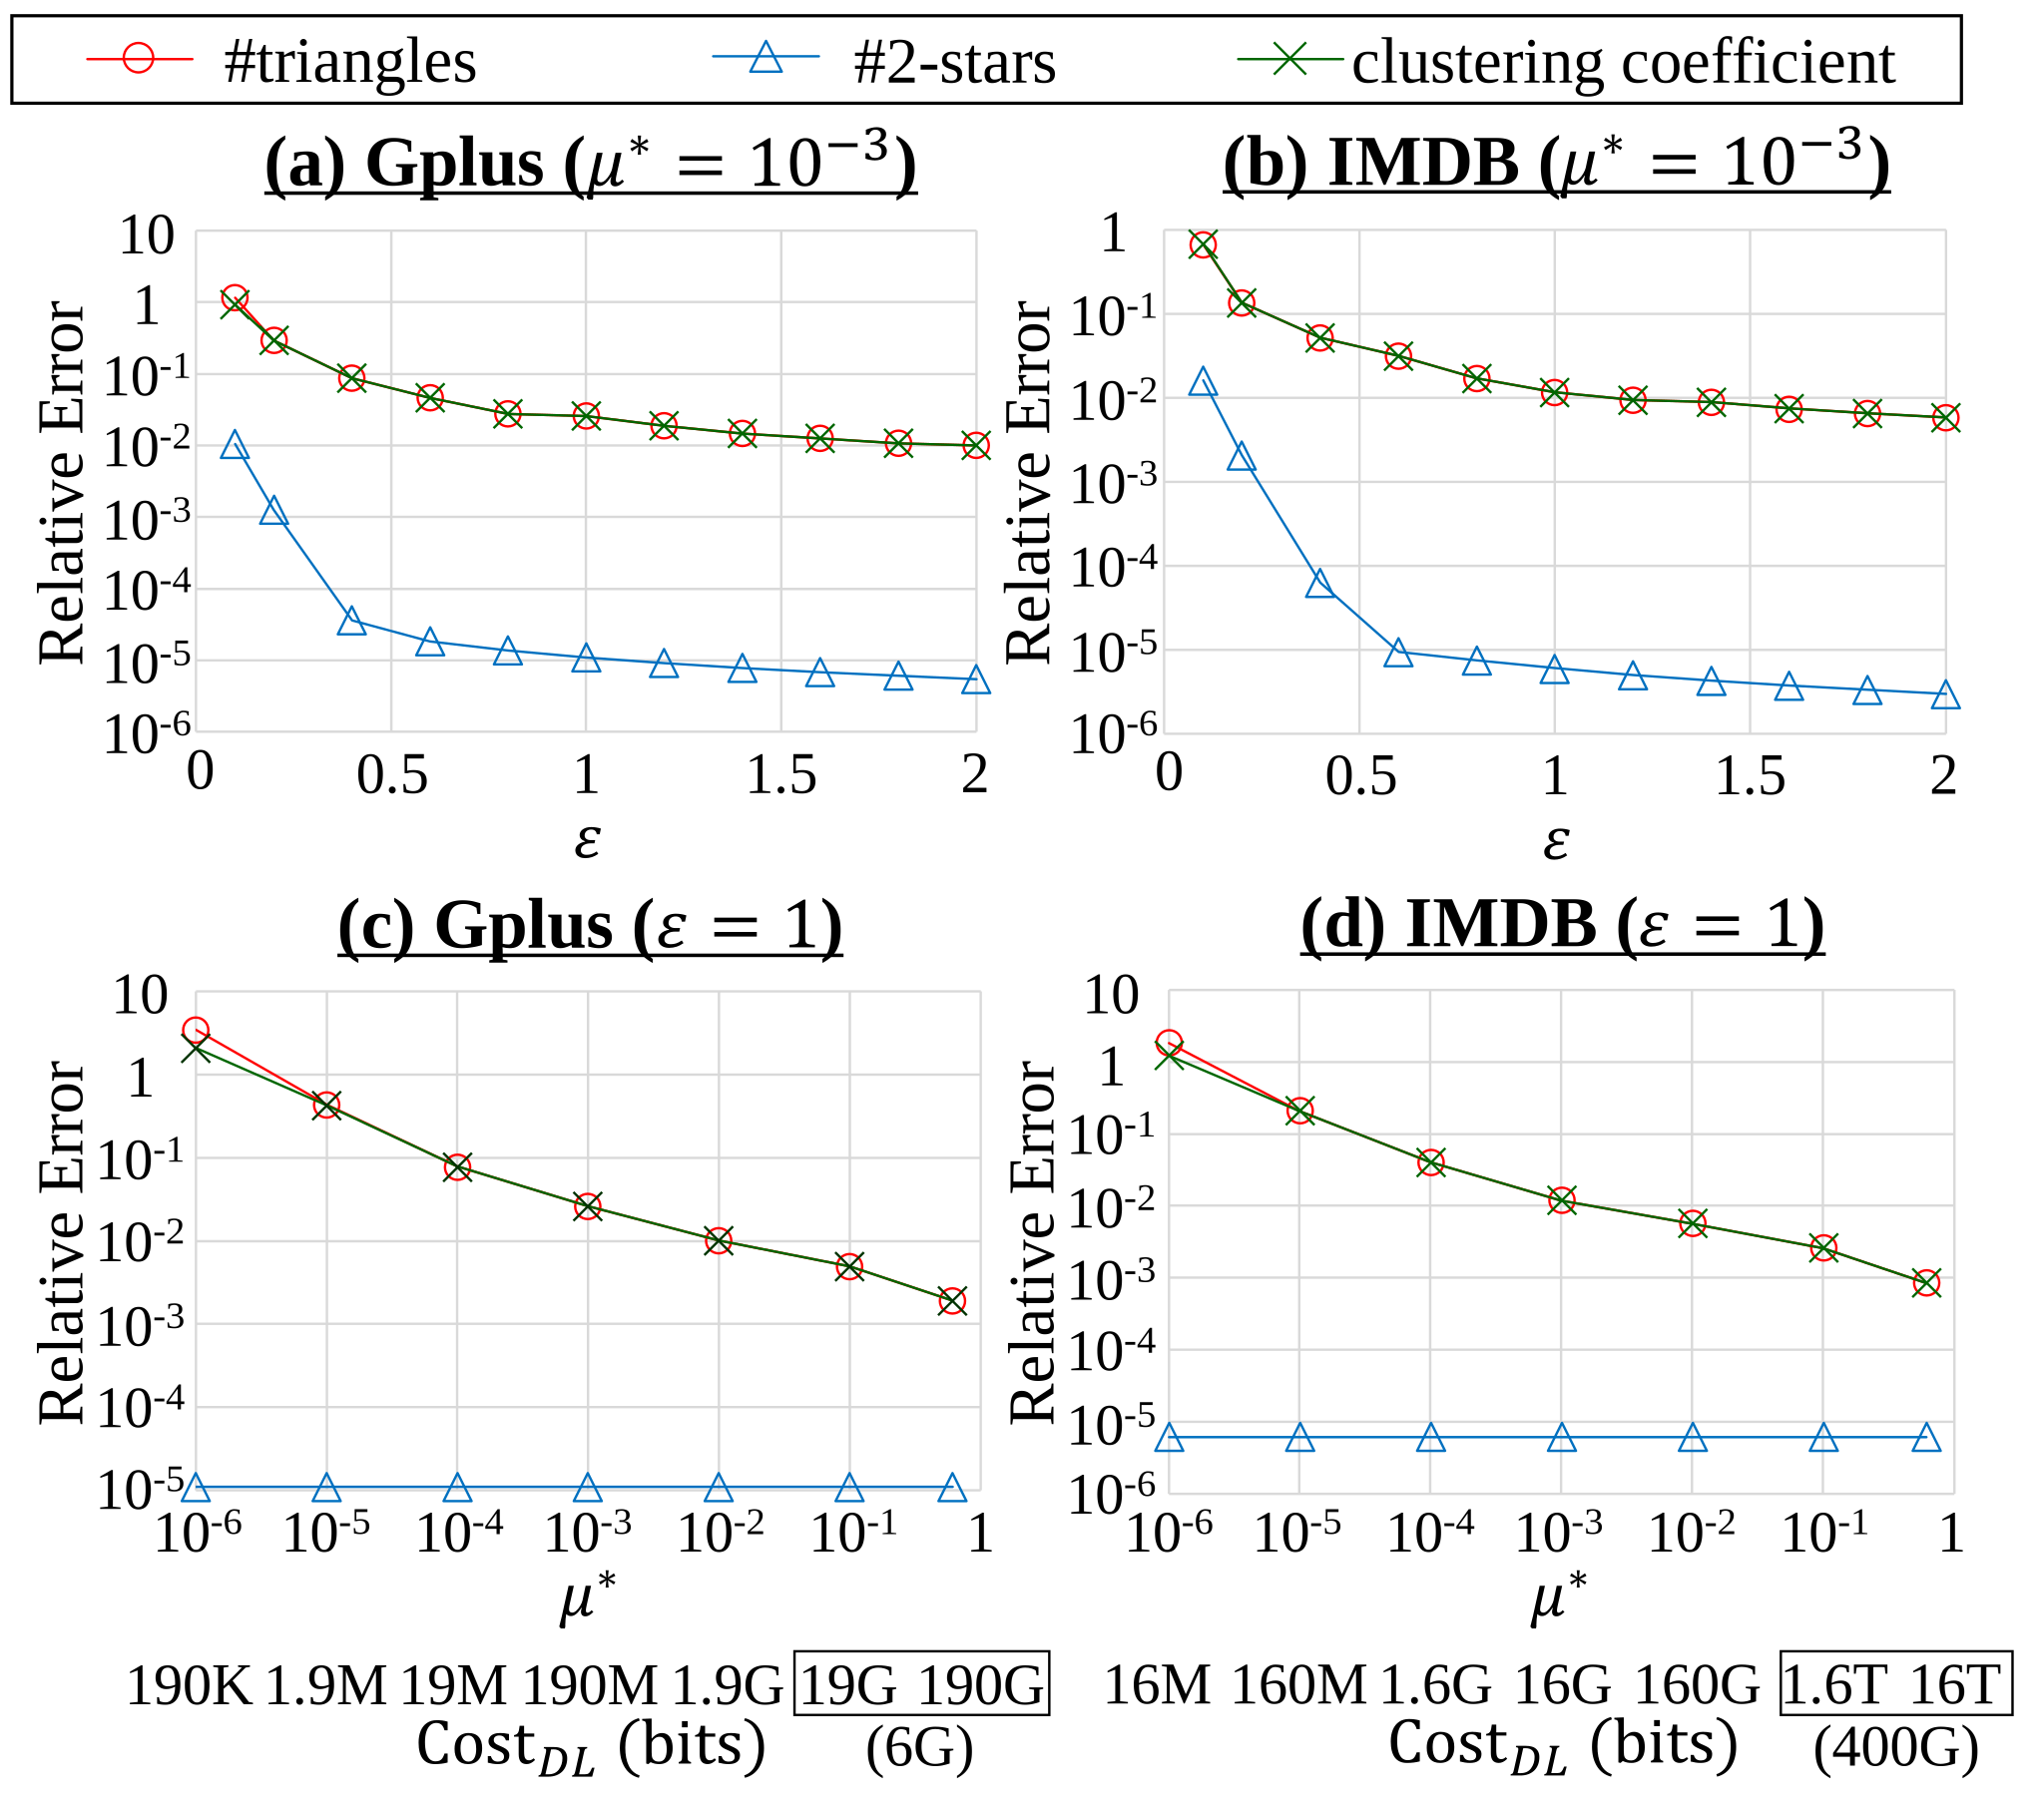
\includegraphics[width=0.99\linewidth]{fig/res5_cluster.pdf}
  
  \caption{Relative errors of \#triangles, \#$2$-stars, and the clustering coefficient in \AlgTwo{} with double clipping.
  $\CostDL$ is calculated by (\ref{chap2-eq:CostDL_F})
  (when $\mu^* \geq 0.1$,
  $\CostDL$ can be $6$ Gbits and $400$ Gbits in \GPlus{} and \IMDB{}, respectively).
  }
  \label{chap2-fig:res5_cluster}
\end{figure}

Figure~\ref{chap2-fig:res5_cluster} shows the relative errors of the triangle count, $2$-star count, and clustering coefficient.
Note that the relative error of the 2-star count is not changed by changing
% $\mu_F$ ($=\mu_O^2=\mu_T^3$)
$\mu^*$
because the 2-star algorithm does not use the ARR.
Figure~\ref{chap2-fig:res5_cluster} shows that the relative error of the $2$-star count is much smaller than that of the triangle count.
This is because each user can count her 2-stars locally (whereas she cannot count her triangles), as described in Section~\ref{chap2-sec:intro}.
Consequently, the relative error of the clustering coefficient is almost the same as that of the triangle count, as the denominator $\hf_{2\star}(G)$ in the clustering coefficient is very accurate.

Note that the clustering coefficient requires the privacy budgets for
calculating both $\hf_\triangle(G)$ and $\hf_{2\star}(G)$
% both the triangle count and $2$-star count
(in Figure~\ref{chap2-fig:res5_cluster}, $2\epsilon$ in total).
% $2\epsilon$ because it needs both the triangle count and $2$-star count.
However, we can accurately
% estimate the $2$-star count
calculate $\hf_{2\star}(G)$
with a very small privacy budget, as shown in Figure~\ref{chap2-fig:res5_cluster}.
Thus, we can accurately estimate the clustering coefficient with almost the same privacy budget as
the triangle count
% $\hf_\triangle(G)$
% by making the privacy budget for the $2$-star count small (e.g., $\epsilon=0.1$ or $0.2$).
by assigning a very small privacy budget (e.g., $\epsilon=0.1$ or $0.2$) for
% the $2$-star count.
$\hf_{2\star}(G)$.

In summary, we can accurately estimate the clustering coefficient as well as the triangle count under edge LDP by using our \AlgTwo{} with double clipping.

\arxiv{
\section{Experiments Using the Barab\'{a}si-Albert Graph Datasets}
\label{chap2-sec:BAmodel}
In Section~\ref{chap2-sec:experiments}, we evaluated our algorithms using two real datasets.
Below we also evaluate our algorithms using a synthetic graph based on the BA (Barab\'{a}si-Albert) graph model~\cite{NetworkScience}, which has a power-law degree distribution.

In the BA graph model, a graph of $n$ nodes is generated by attaching new nodes one by one.
% Each node has $m \in \nnints$ edges, 
Each new node is connected to $m \in \nnints$ existing nodes, 
and each edge is connected to an existing node with probability proportional to its degree.
We used NetworkX \cite{Hagberg_SciPy08}, a Python package for complex networks, to generate synthetic graphs based on the BA graph model.

We generated a graph $G=(V,E)$ with the same number of nodes as
% the Google+ dataset~\cite{McAuley_NIPS12} (\GPlus{});
\GPlus{}; i.e., $n=107614$ nodes.
% and $m=$
For the number $m$ of edges per node, we set $m=50$, $114$, or $500$.
% Note that the BA graph with $m=114$ has almost the average degree as \GPlus{}.
% When $m=114$, most nodes have the degree of $114$, which is the average degree in \GPlus{}. 
% Thus, we can see the difference between them.
Using these graphs, we evaluated our three algorithms with double clipping.
We set parameters in the same as Section~\ref{chap2-sec:experiments}; i.e.,
$\alpha = 150$, $\beta = 10^{-6}$, $\epsilon_0 = \frac{\epsilon}{10}$, and $\epsilon_1 = \epsilon_2 = \frac{9\epsilon}{20}$.
% We ran each algorithm $10$ times, and averaged the relative error over the $10$ cases.
For each algorithm, we averaged the relative error over $10$ runs.

% \begin{figure}[t]
%   \centering
%   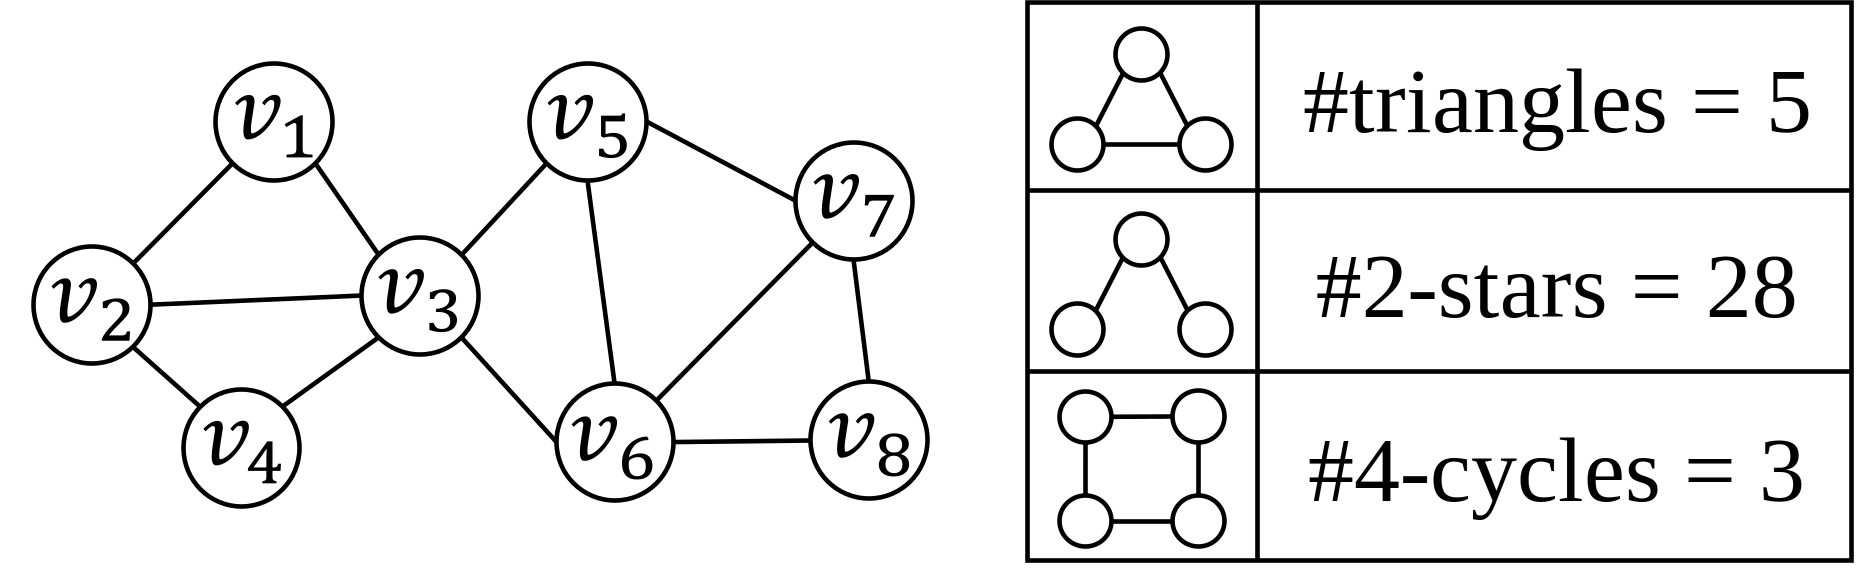
\includegraphics[width=0.95\linewidth]{fig/subgraphs.pdf}
%   
%   \caption{Subgraphs used in our theoretical analysis.}
%   \label{chap2-fig:subgraphs}
% \end{figure}

Figure~\ref{chap2-fig:resA_BAGraph} shows the results, where $\epsilon=1$ and
% $\mu_F$ ($= \mu_O^2 = \mu_T^3$)
$\mu^* = 10^{-3}$.
We observe that \AlgTwo{} significantly outperforms \AlgOne{} and \AlgThree{} when $m=500$, and that \AlgTwo{} performs almost the same as \AlgOne{} when $m=50$ or $114$.

To examine the reason for this, we also decomposed the estimation error into two components (the first error by empirical estimation and the second error by the Laplacian noise) in the same way as Figure~\ref{chap2-fig:res3_emp_Lap}.
Figure~\ref{chap2-fig:resA_BAGraph_emp_Lap} shows the results.
% In addition, we calculated the number $C_4$ of $4$-cycles in the BA graph.
We also show in Table~\ref{chap2-tab:resA_4cycles} the number $C_4$ of $4$-cycles in each BA graph ($m=50$, $114$, or $500$) and \GPlus{}.

From Figure~\ref{chap2-fig:resA_BAGraph_emp_Lap} and Table~\ref{chap2-tab:resA_4cycles}, we can explain Figure~\ref{chap2-fig:resA_BAGraph} as follows.
The BA graphs with $m=50$ and $114$ have a much smaller number $C_4$ of $4$-cycles than \GPlus{}, as shown in Table~\ref{chap2-tab:resA_4cycles}.
Consequently,
% the error caused by
the Laplacian noise is relatively large and dominant for these two graphs, as shown in Figure~\ref{chap2-fig:resA_BAGraph_emp_Lap}.
In particular,
% the relative error of
the Laplacian noise is the largest in \AlgThree{} because it cannot effectively reduce the global sensitivity by double clipping, as explained in Section~\ref{chap2-sec:double_clip}.
In contrast, the BA graph with $m=500$ has a larger number $C_4$ of $4$-cycles than \GPlus{}, and therefore the Laplacian noise is not dominant (except for \AlgThree{}).
This explains the results in Figure~\ref{chap2-fig:resA_BAGraph}.

These results
% , along with Section~\ref{chap2-sec:experiments},
% Our experimental results in Appendix~\ref{chap2-sec:BAmodel} and Section~\ref{chap2-sec:experiments},
show that \AlgTwo{} outperforms \AlgOne{} especially when the number $C_4$ of $4$-cycles is large.
As we have shown in Section~\ref{chap2-sec:experiments} and Appendix~\ref{chap2-sec:BAmodel}, $C_4$ is large in a large graph (e.g., $n \approx 10^6$) or dense graph (e.g., \GPlus{}, BA graph with $m=500$).

\begin{figure}[t]
  \centering
  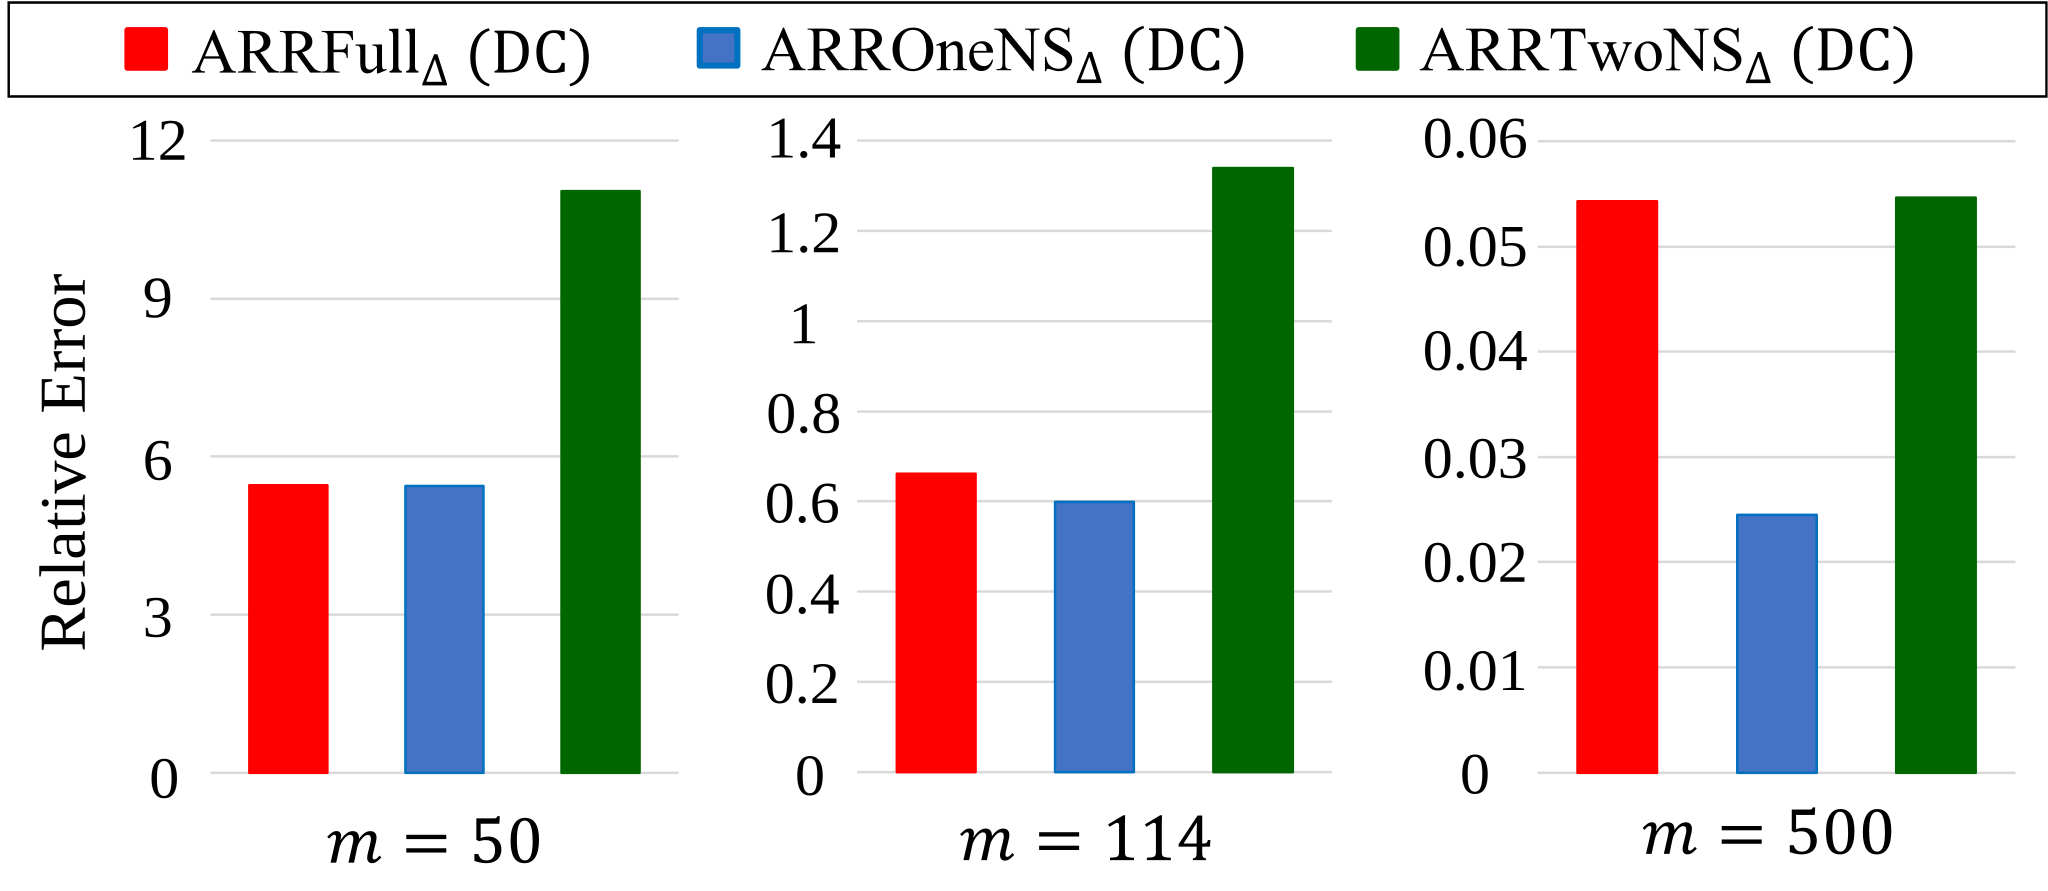
\includegraphics[width=0.99\linewidth]{fig/resA_BAGraph.pdf}
  
  \caption{Relative error of our three algorithms with double clipping in the BA graphs ($n=107614$, $\epsilon=1$, $\mu^* = 10^{-3}$).}
  \label{chap2-fig:resA_BAGraph}
% \end{figure}
\vspace{5mm}
% \begin{figure}[t]
  \centering
  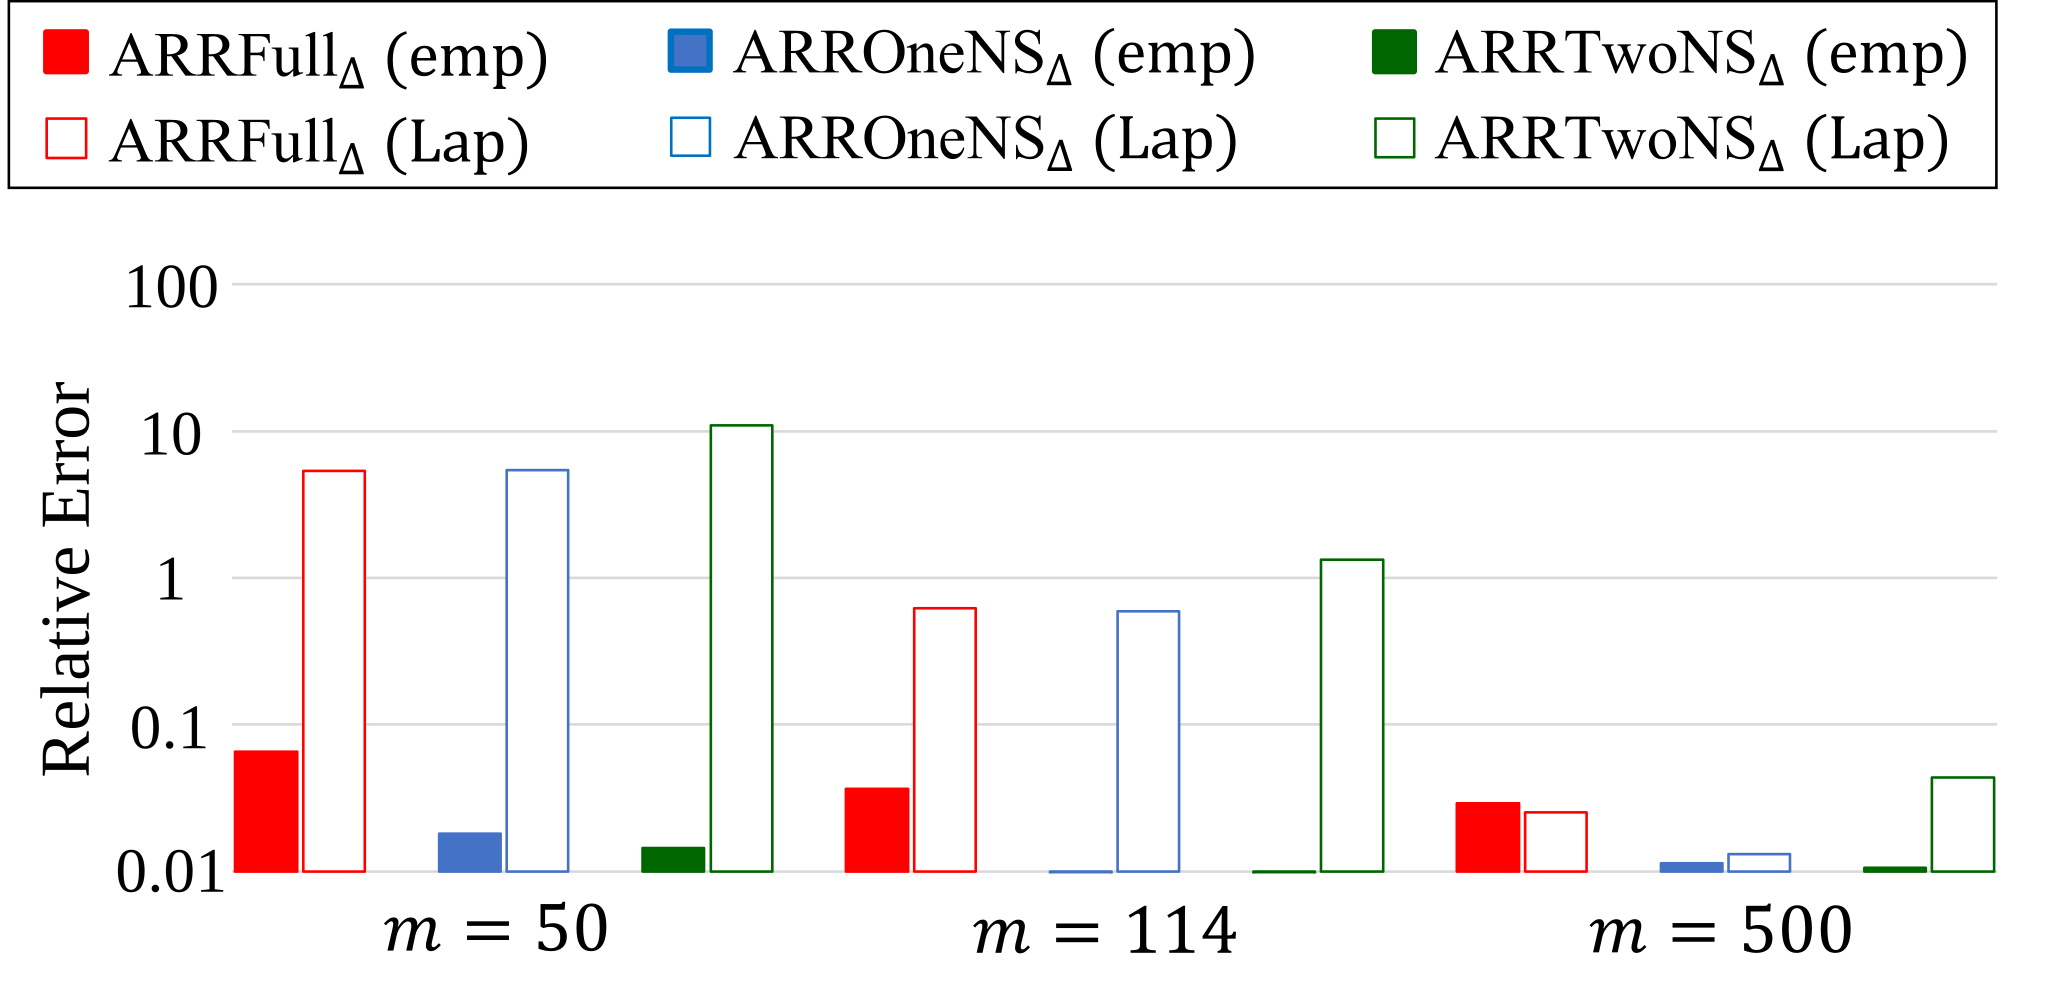
\includegraphics[width=0.95\linewidth]{fig/resA_BAGraph_emp_Lap.pdf}
  
  \caption{Relative error of empirical estimation and the Laplacian noise in our three algorithms with double clipping in the BA graphs ($n=107614$, $\epsilon=1$, $\mu^* = 10^{-3}$).}
  \label{chap2-fig:resA_BAGraph_emp_Lap}
\end{figure}

\section{Edge Clipping and Noisy Triangle Clipping}
\label{chap2-sec:EC_DC}
% \smallskip
% \noindent{\textbf{Edge Clipping and Noisy Triangle Clipping.}}~~
In Section~\ref{chap2-sec:experiments}, we showed that our double clipping significantly reduces the estimation error.
To investigate the effect of
% adaptive
edge clipping and noisy triangle clipping independently, we also performed the following ablation study.

We evaluated our three algorithms with only
% adaptive
edge clipping; i.e., each user calculates a noisy degree $\td_i$ (possibly with edge clipping) and then adds $\Lap(\frac{\td_i}{\epsilon_2}$) to her noisy triangle count.
Then we compared them with our algorithms with double clipping and without clipping.

\begin{table}[t]
\caption{\#$4$-cycles $C_4$ in each graph dataset.}
\centering
\hbox to\hsize{\hfil
\begin{tabular}{l|l|l|l|l}
\hline
		&	$m=50$   &  $m=114$   &  $m=500$   &  \GPlus{}\\
\hline
$C_4$   &   $8.8 \times 10^8$ &  $1.7 \times 10^{10}$ &   $3.1 \times 10^{12}$ &   $2.8 \times 10^{12}$\\
\hline
\end{tabular}
\hfil}
\label{chap2-tab:resA_4cycles}
\end{table}

\begin{figure}[t]
  \centering
  \includegraphics[width=0.99\linewidth]{fig/res2_w_Lap_EC.pdf}
  
  \caption{Relative error of our three algorithms without clipping (``$d_{max}$''), with only edge clipping (``EC''), and double clipping (``DC'') when $\epsilon=1$ and $\mu^* = 10^{-6}$ or $10^{-3}$ ($n=107614$ in \GPlus{}, $n=896308$ in \IMDB{}).}
  \label{chap2-fig:res2_w_Lap_EC}
\end{figure}

Figure~\ref{chap2-fig:res2_w_Lap_EC} shows the results, where $\epsilon=1$, $\mu^* = 10^{-6}$ or $10^{-3}$, and ``EC'' represents our algorithms with only
% adaptive
edge clipping.
We observe that ``EC''
% (only edge clipping)
outperforms ``$d_{max}$'' (w/o clipping) and is outperformed by ``DC'' (double clipping).
The difference between ``EC'' and ``DC'' is significant especially when $\mu^* = 10^{-6}$ (``DC'' is smaller than $\frac{1}{100}$ of ``EC'').
This is because our noisy triangle clipping reduces the global sensitivity by using a small value of
$\mu^*$. 
% $\mu_F$ ($=\mu_O^2 = \mu_T^3$).
From Figure~\ref{chap2-fig:res2_w_Lap_EC}, we conclude that each component (i.e.,
% adaptive
edge clipping, noisy triangle clipping) is essential in our double clipping.

\section{Proof of Proposition~\ref{chap2-prop:seq_comp_edge_LDP}}
\label{chap2-sec:proof_seq_comp_edge_LDP}
Let $\calR_i(\bma_i) = (\calR_i^1(\bma_i), \calR_i^2(M_i)(\bma_i))$ be the
randomizer used by user $v_i$ in the composition. To establish that
$\calR_i(\bma_i)$ satisfies $\epsilon$-edge LDP for every $v_i \in V$, we will
prove that~\eqref{chap2-eq:edge_LDP} holds for $\calR_i(\bma_i)$. To do this, first write
\begin{align*}
  &\;\Pr[(\calR_i^1(\bma_i), \calR_i^2(M_i)(\bma_i)) = (r_i^1, r_i^2)] = \\
  &\qquad\Pr[\calR_i^1(\bma_i) = r_i^1]\Pr[\calR_i^2(M_i)(\bma_i) = r_i^2 | \calR_i^1(\bma_i) = r_i^1] \\
  &\qquad\Pr[\calR_i^1(\bma_i) = r_i^1]\Pr[\calR_i^2(M_i)(\bma_i) = r_i^2 | M_i = \lambda_i(r_i^1)],
\end{align*}
where the last equality follows because $M_i = \lambda_i(\calR_i^1(\bma_i))$ for a post-processing algorithm $\lambda_i$.
Notice that the same equalities are true when we replace $\bma_i$ with $\bma_i'$.
Because $\calR_i^1$ and $\calR_i^2(M_i)$ (for any $M_i$) satisfy $\epsilon_1, \epsilon_2$-edge LDP, respectively,
we have
\begin{align*}
  &\;\Pr[\calR_i^1(\bma_i) = r_i^1]\Pr[\calR_i^2(M_i)(\bma_i) = r_i^2 | M_i = \lambda_i(r_i^1)] \\
  &\qquad\leq e^{\epsilon_1}\Pr[\calR_i^1(\bma_i') = r_i^1]e^{\epsilon_2}\Pr[\calR_i^2(\bma_i') = r_i^2 | M_i = \lambda_i(r_i^1)] \\
  &\qquad= e^{\epsilon_1 + \epsilon_2} \Pr[(\calR_i^1(\bma_i'), \calR_i^2(M_i)(\bma_i')) = (r_i^1, r_i^2)].
\end{align*}
This establishes the result. \qed

\section{Proof of Statements in Section~\ref{chap2-sec:algorithms}}
\label{chap2-sec:proof_algorithms}
\subsection{Proof of Theorem~\ref{chap2-thm:privacy_algorithms}}
Let $\bma_i, \bma'_i \in \{0,1\}^n$ be two neighbor lists that differ in one bit.
Let $t'_i$, $s'_i$, and $w'_i$ be respectively the values of $t_i$ (line 11 of Algorithm~\ref{chap2-alg:unify}), $s_i$ (line 12), and $w_i$ (line 13) when the neighbor list of user $v_i$ is $\bma'_i$.
Let $\Delta w_i = |w'_i - w_i|$.
Then we have $t'_i - t_i \in [0,d_{max}]$ and $s'_i - s_i \in [0,d_{max}]$, and therefore $\Delta w_i = |(t'_i - t_i) - \mu^* \rho(s'_i - s_i)| \leq d_{max}$.

Since we add
$\Lap\left(\frac{d_{max}}{\epsilon_2}\right)$
to $w_i$, the second round provides $\epsilon_2$-edge LDP.
The first round uses $ARR_{\epsilon_1,\mu}$ and provides $\epsilon_1$-edge LDP.
Thus, by sequential composition (Proposition~\ref{chap2-prop:seq_comp_edge_LDP}),
Algorithm~\ref{chap2-alg:unify} provides ($\epsilon_1+\epsilon_2$)-edge LDP in total.
It also provides ($\epsilon_1+\epsilon_2$)-relationship DP because it uses only the lower-triangular part of $\bmA$ (Proposition~\ref{chap2-prop:edge_LDP_entire_edge_LDP}).
% \ji{We should formally state the lower-triangular relationship DP result somewhere, I think maybe add it to proposition 1.}
\qed

\subsection{Proof of Theorem~\ref{chap2-thm:l2loss_algorithms}}
\label{chap2-sub:prrof_l2loss_algorithms}
% \paragraph{Unbiased Estimators}
% \smallskip
\noindent{\textbf{Unbiased Estimators.}}~~First, we will show that $\hf_\triangle(G)$ satisfies
$\E[\hf_\triangle(G)] = f_\triangle(G)$ for all $G \in \calG$, in \AlgOne{}, \AlgTwo{}, \AlgThree{}.
Regardless of algorithm, we have
\begin{align}
  &\;\E[\hf_\triangle(G)] \nonumber \\
  &= \frac{1}{\mu^*(1-\rho)}\sum_{i=1}^n \E[w_i] \nonumber \\
  &= \frac{1}{\mu^*(1-\rho)}\sum_{i=1}^n \E[t_i - \mu^* \rho s_i] \nonumber \\
  &= \frac{1}{\mu^*(1-\rho)}\sum_{i=1}^n \sum_{\substack{1 \leq j < k < i \leq n \\ a_{i,j} = a_{i,k} = 1}} \E[\textbf{1}_{(v_j, v_k) \in M_i} - \mu^* \rho],
  \label{chap2-eq:unbias_1}
\end{align}
where $\rho = e^{-\epsilon_1}$, and the quantites $\mu^*, t_i, s_i$ are defined in
Algorithm~\ref{chap2-alg:unify}. Given that $a_{i,j} = a_{i,k} = 1$, we have that
$\Pr[(v_i, v_j) \in E'] = \Pr[(v_i, v_k) \in E'] = \mu$ by definition of ARR.
Furthermore,
% $\Pr[(v_i, v_k) \in E'] = \mu$ if $a_{i,k} = 1$, and $\Pr[(v_i, v_k) \in E'] = \mu\rho$ otherwise.
$\Pr[(v_j, v_k) \in E'] = \mu$ if $a_{j,k} = 1$, and $\Pr[(v_j, v_k) \in E'] = \mu\rho$ otherwise.
Examining~\eqref{chap2-eq:M_i_I},~\eqref{chap2-eq:M_i_II}, and~\eqref{chap2-eq:M_i_III}, we have
\[
  \Pr[(v_j, v_k) \in M_i] =
  \begin{cases}
    \mu^* & a_{j,k} = 1 \\
    \mu^*\rho & a_{j,k} = 0
  \end{cases}
\]
for all the three algorithms (note that $\mu^* = \mu$, $\mu^2$, and $\mu^3$ in \AlgOne{}, \AlgTwo{}, \AlgThree{}, respectively).
Thus, $\E[\textbf{1}_{(v_j, v_k) \in M_i}] = \mu^* (\rho + (1-\rho) a_{j,k})$
($= \mu^*$ if $a_{i,j}=1$ and $\mu^* \rho$ if $a_{i,j}=0$).
Plugging into~\eqref{chap2-eq:unbias_1}, we have
\begin{align*}
  &\;\E[\hf_\triangle(G)] \\
  &=
  \frac{1}{\mu^*(1-\rho)}\sum_{i=1}^n \sum_{\substack{1 \leq j < k < i \leq n \\ a_{i,j} = a_{i,k} =
  1}} \mu^*(\rho + (1-\rho)a_{j,k}) - \mu^* \rho \\
  &= \frac{1}{\mu^*(1-\rho)}\sum_{i=1}^n \sum_{\substack{1 \leq j < k < i \leq n \\ a_{i,j} = a_{i,k} =
  1}} \mu^*(1-\rho)a_{j,k} \\
  &= \sum_{i=1}^n \sum_{\substack{1 \leq j < k < i \leq n \\ a_{i,j} = a_{i,k} =
  1}} a_{j,k} \\
  &= f_\triangle(G).
\end{align*} 
Thus, $\hf_\triangle(G)$ is unbiased. \qed

% \paragraph{$l_2^2$-Loss of Estimators}
\smallskip
\noindent{\textbf{$l_2$ Loss of Estimators.}}~~Using bias-variance decomposition, we have
for any graph $G$,
\begin{align*}
  l_2^2(f_\triangle(G), \hf_\triangle(G)) &= \E[(\hf_\triangle(G) - f_\triangle(G))^2] \\
  &= \E[(f_\triangle(G) - \E[\hf_\triangle(G)])^2] + \V[\hf_\triangle(G)] \\
  &= \V[\hf_\triangle(G)],
\end{align*}
where the last step follows because $\hf$ is unbiased.
Since $\hf_\triangle(G) = \frac{1}{\mu^*(1-\rho)} \sum_{i=1}^n \hw_i$, we have
% Substituting for $\hf_\triangle(G)$, we see
\begin{align}
  &\;\V[\hf_\triangle(G)] \nonumber \\
  &= \frac{1}{(\mu^*)^2(1-\rho)^2}\V\left[\sum_{i=1}^n \hw_i\right] \nonumber \\
  &= \frac{1}{(\mu^*)^2(1-\rho)^2}\V\left[\sum_{i=1}^n w_i + \Lap\left(\frac{d_{max}}{\epsilon_2} \right)\right] \nonumber \\
  &= \frac{1}{(\mu^*)^2(1-\rho)^2}\left(\V\left[\sum_{i=1}^n w_i\right] +
  n\V\left[\Lap\left(\frac{d_{max}}{\epsilon_2}\right)\right]\right) \nonumber \\
  &= \frac{1}{(\mu^*)^2(1-\rho)^2}\left(\V\left[\sum_{i=1}^n w_i\right] +
  2n\frac{d_{max}^2}{\epsilon_2^2}\right), \label{chap2-eq:inter_var}
\end{align}
where the
% third
fourth
line follows from independence of the added of Laplace noise.
Now, we will prove bounds on $\V[\sum_{i=1}^nw_i]$ for \AlgOne{}, \AlgTwo{}, and
\AlgThree{}. In the following, we let $S_k(G)$ be the number of $k$-stars in
$G$ and $C_4(G)$ be the number of $4$-cycles in $G$
% , and $P_3(G)$ be the number of
% $3$-paths in $G$.

% \paragraph{Bounding the Variance in \AlgOne{}}
\smallskip
\noindent{\textbf{Bounding the Variance in \AlgOne{}.}}~~In \AlgOne{}, $M_i$ is defined by \eqref{chap2-eq:M_i_I}. Thus we have
% we have $M_i = E'$, so we can write
\begin{align*}
  \sum_{i=1}^n w_i &= \sum_{i=1}^n \sum_{\substack{1 \leq j < k < i \leq n \\ a_{i,j} = 1, a_{i,k} = 1}} \textbf{1}_{(v_j, v_k) \in M_i} \\
  &= \sum_{1 \leq j < k \leq n} \sum_{k < i \leq n} a_{i,j} a_{i,k} \textbf{1}_{(v_j, v_k) \in E'} \\
  &= \sum_{1 \leq j < k \leq n} \textbf{1}_{(v_j, v_k) \in E'}\sum_{k < i \leq n} a_{i,j} a_{i,k}
\end{align*}
For $j < k$, we introduce the constant $c_{jk} = \sum_{k < i \leq n} a_{i,j} a_{i,k}$. Notice that
for any choice of $j$ and $k$, $\textbf{1}_{(v_j, v_k) \in E'}$ for $1 \leq j \leq k$ are mutually independent,
because all edges in $E'$ are mutually independent. Furthermore, the indicator
$\textbf{1}_{(v_j, v_k) \in E'}$ is a Bernoulli random variable with parameter
either $\mu$ or $\mu\rho$, and in either case, $\V[\textbf{1}_{(v_j, v_k) \in
E'}] \leq \mu$. We have
\begin{align*}
  \V\left[\sum_{i=1}^n w_i\right]
  &= \V\left[\sum_{1 \leq j < k \leq n} \textbf{1}_{(v_j, v_k) \in E'}c_{jk}\right] \\
  &= \sum_{1 \leq j < k \leq n} \V[\textbf{1}_{(v_j, v_k) \in E'}c_{jk}] \\
  &= \sum_{1 \leq j < k \leq n} \mu c_{jk}^2.
\end{align*}
By Lemma~\ref{chap2-lem:c_ij_4cycle_2star} (which is shown at the end of Appendix~\ref{chap2-sub:prrof_l2loss_algorithms}), we have $\sum_{1 \leq j < k \leq n} c_{jk}^2 \leq 2 C_4(G) + S_2(G)$.
Plugging into~\eqref{chap2-eq:inter_var} (and substituting $\mu^* = \mu$), we obtain
\begin{align*}
  \V[\hf_\triangle(G)]
  &= \frac{1}{(1-\rho)^2}\left(\frac{1}{\mu}(2C_4(G) + S_2(G)) +
  2n\frac{d_{max}^2}{\mu^2\epsilon_2^2}\right). \\
\end{align*}
This establishes the result. \qed

% \paragraph{Bounding the Variance in \AlgTwo{}}
\smallskip
\noindent{\textbf{Bounding the Variance in \AlgTwo{}.}}~~In \AlgTwo{}, for a fixed
$v_i \in V$, we have $(v_j, v_k) \in M_i$ if and only if
$j < k < i$, $(v_j, v_k) \in E'$, and $(v_i, v_k) \in E'$ from~\eqref{chap2-eq:M_i_II}. Thus,
\begin{align*}
\sum_{i=1}^n w_i &= \sum_{i=1}^n~\sum_{\substack{1 \leq j < k < i \leq n \\
a_{i,j} = 1, a_{i,k} = 1}} \textbf{1}_{(v_j, v_k) \in M_i} \\
&= \sum_{1 \leq j < k < i \leq n}
\textbf{1}_{(v_j, v_k) \in E'} a_{i,j}a_{i,k}\textbf{1}_{(v_i, v_k) \in E'}
\end{align*}

Define the random variable $F_{ijk} = \textbf{1}_{(v_j, v_k) \in
E'} \textbf{1}_{(v_i, v_k) \in E'}$. Substituting, we have
\begin{align*}
  \sum_{i=1}^n w_i &= \sum_{1 \leq j < k < i \leq n} a_{i,j} a_{i,k}F_{ijk} \\
  \V\left[\sum_{i=1}^n w_i\right]
  &= \sum_{\substack{1 \leq j < k < i \leq n \\ 1 \leq j' < k' <
  i' \leq n}} a_{i,j} a_{i,k} a_{i',j'} a_{i',k'} \cov(F_{ijk}, F_{i'j'k'}).
\end{align*}

The set $\{i,i',j,j',k,k'\}$ when $j < k < i$ and $j' < k' < i'$ can take between
three and six distinct values.
If $\{i,i', j,j', k,k'\}$ takes five or more distinct values, then $F_{ijk}$ and
$F_{i'j'k'}$ involve distinct edges and are independent random variables. Thus,
$\cov(F_{ijk}, F_{i'j'k'}) = 0$. Otherwise, the events are not independent, and we will
use the upper bound $\cov(F_{ijk}, F_{i'j'k'}) \leq \E[F_{ijk}F_{i'j'k'}]
% \leq
=
\Pr[F_{ijk} = F_{i'j'k'} = 1]$, which holds because the $F_{ijk}$ have domain $\{0,1\}$.
Thus,
% \[
\begin{align*}
&\;\V\left[\sum_{i=1}^n w_i \right] \\
&\leq
  \sum_{\substack{1 \leq j < k < i \leq n \\ 1 \leq j' < k' <
  i' \leq n \\ |\{i,j,k,i',j',k'\}| = 3 \text{ or } 4}} a_{i,j} a_{i,k} a_{i',j'} a_{i',k'} \Pr[F_{ijk} = F_{i'j'k'} = 1].
% \]
\end{align*}

Define a choice of $(i,j,k,i',j',k') \in [n]^6$ to be a \emph{valid} choice if
$j < k < i$, $j' < k' < i'$ (ordering requirement),
$a_{i,k} = a_{i,j} = a_{i',j'} = a_{i', k'} = 1$ (edge requirement), and
$3 \leq \{i,i',j,j',k,k'\} \leq 4$ (size requirement). We can write the above sum as
\[
  \V\left[\sum_{i=1}^n w_i \right] \leq
  \sum_{i,i',j,j',k,k'\text{ valid}} \Pr[F_{ijk} = F_{i'j'k'} = 1].
\]

In the above sum, each valid choice implies there exists
a subgraph of $G$ that associates
each of $\{v_i, v_{i'}, v_j, v_{j'}, v_k, v_{k'}\}$ with one node in the subgraph and contains edges $(v_i, v_j), (v_i, v_k), (v_{i'}, v_{j'}), (v_{i'}, v_{k'})$.
Conversely,
each
% labeled
subgraph of $G$ of three or four nodes can have a certain
number of valid choices mapped to it. For each
subgraph, we now go over the number of possible valid choices that can map to it:

\begin{enumerate}
    \item 4-cycle: By ordering, either $i$ or $i'$ is mapped to the node of the 4-cycle
    with maximal
    index. WLOG, suppose $i$ is mapped to this node. By edge requirements, $i'$ has an index equal
    to the opposite node in the $4$-cycle. By ordering, there is now one
    way to map $j,j',k,k'$. Thus, each 4-cycle can be associated with
    % at most
    $\mathbf{2}$ valid choices.
    \item 3-path: Consider the middle node $v_\ell$ in the 3-path (path graph on 4 nodes) that has
    the second-largest index.
    %higher index than the other middle node.
    By ordering, either $i=\ell$ or $i' = \ell$.
    WLOG, suppose $i = \ell$. Then, by the edge requirement $a_{i',j'} = a_{i', k'} = 1$, the middle node other than $v_\ell$ is
    $i'$. However, this means either $i = j'$ or $i = k'$, and we have $j' > i'$ or $k' > i'$.
    This violates the order requirement, and therefore there are $\textbf{0}$ valid choices.
    \item 3-star: By edge requirement, both $i,i'$ map to the central node in the 3-star.
    $j,j',k,k'$ can map to the other three nodes in any way that satisfies ordering.
    Suppose the three nodes are $v_{a}, v_{b}, v_c$ with $a < b < c$.
    % Each of
    Only one of
    the three nodes can be duplicated in this mapping.
    %once.
    %and if for example
    For example, if
    $a$ is duplicated, then both
    %$k,k'$
    $j$ and $j'$
    map to $v_a$, and there are two remaining choices
    for how to map
    %$j,j'$.
    $k$ and $k'$.
    % This means
    Thus,
    each $S_3$ can
    be associated with
    %at most
    $\mathbf{6}$ valid choices.
    \item Triangle: Either $i$ or $i'$ maps to the maximal node in the triangle
    by ordering. WLOG, suppose $i$ does. By the edge requirement, $i'$ maps
    to a different node. However, this means $i = k'$ or $i=j'$, so $k' > i'$,
    contradicting ordering. Thus, there are $\textbf{0}$ valid choices.
    \item 2-star: By edge requirements, both $i$ and $i'$ map to the central node in the
    2-star. We then have just one mapping for the remaining indices. Thus, there
    is $\textbf{1}$ valid choice.
\end{enumerate}
Figure~\ref{chap2-fig:associated_subgraphs} shows an example of two 4-cycles, six 3-stars, and one 2-stars.
We can see that the other possible subgraphs on 3 or 4 nodes are immediately
ruled out because they have too many or too few edges, violating edge requirements.

\begin{figure}[t]
  \centering
  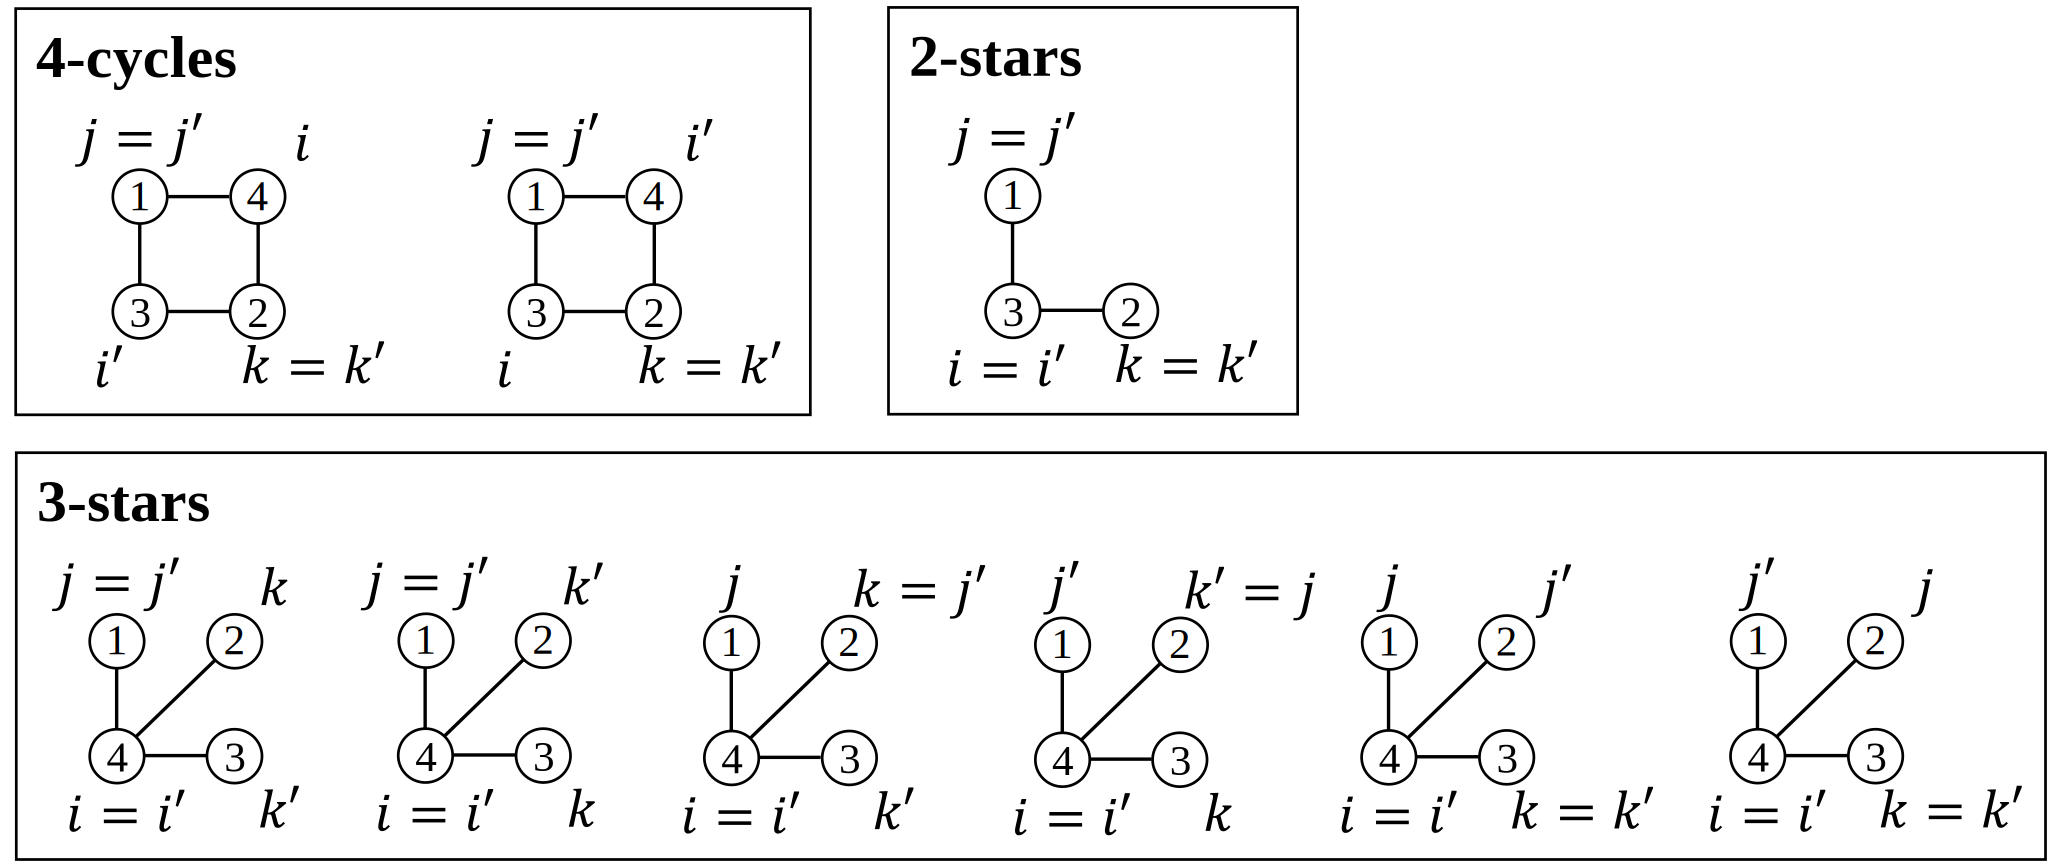
\includegraphics[width=0.99\linewidth]{fig/associated_subgraphs.pdf}
  
  \caption{Examples of two 4-cycles, six 3-stars, and one 2-stars.}
  \label{chap2-fig:associated_subgraphs}
\end{figure}

In the following, let $P(i,j,k)$ be the event that $F_{ijk} = F_{i'j'k'} = 1$.
Observing Figure~\ref{chap2-fig:four-cycle}, we can see that in both possible ways in
which a valid choice maps to a $4$-cycle, then $P(i,j,k)$ holds when at least $3$
edges in $E'$ are present. Each edge in $E'$ is independent,
and is present with probability at most $\mu$. Thus, $\Pr[P(i,j,k)] \leq \mu^3$.
Next, if a valid choice maps to a $3$-star, then $P(i,j,k)$ implies at least $3$
edges in $E'$ are present. Thus, $\Pr[P(i,j,k) = 1] \leq \mu^3$.
Finally, if a valid choice maps to a $2$-star, then $P(i,j,k) = 1$
if and only if $2$ edges in $E'$ are present. Thus, $\Pr[P(i,j,k) = 1] \leq \mu^2$.

Putting this together,
\[
  \V\left[\sum_{i=1}^n w_i\right] \leq 2 C_4(G) \mu^3 + 6 S_3(G) \mu^3 + S_2(G) \mu^2.
\]
Plugging into~\eqref{chap2-eq:inter_var}, we get
% \[
\begin{align*}
  &\;\V[\hf_\triangle(G)] \\
  &\leq \frac{1}{(1-\rho)^2} \left(\frac{1}{\mu}(2C_4(G) + 6S_3(G)) + \frac{1}{\mu^2} S_2(G) + 2n\frac{d_{max}^2}{\mu^4\epsilon_2^2}\right).
% \]
\end{align*}
This establishes the result. \qed

\smallskip
\noindent{\textbf{Bounding the Variance in \AlgThree{}.}}~~In \AlgThree{}, for a fixed
$v_i \in V$, we have $(v_j, v_k) \in M_i$ if and only if
$j < k < i$, $(v_j, v_k) \in E'$, $(v_i, v_k) \in E'$, and $(v_i, v_k) \in E'$
from~\eqref{chap2-eq:M_i_III}. Thus,
\begin{align*}
\sum_{i=1}^n w_i &= \sum_{i=1}^n~\sum_{\substack{1 \leq j < k < i \leq n \\
a_{i,j} = 1, a_{i,k} = 1}} \textbf{1}_{(v_j, v_k) \in M_i} \\
&= \sum_{1 \leq j < k < i \leq n}
a_{i,j}a_{i,k}\textbf{1}_{(v_j, v_k) \in E'} \textbf{1}_{(v_i, v_k) \in E'}\textbf{1}_{(v_j, v_k) \in E'}.
\end{align*}

Define the random variable $F_{ijk} = \textbf{1}_{(v_j v_k) \in E'}
\textbf{1}_{(v_i, v_k) \in E'} \allowbreak \textbf{1}_{(v_j, v_k) \in E'}$. Following the same
steps as those in the proof of \AlgTwo{}, we have
\begin{align*}
  \V\left[\sum_{i=1}^n w_i\right]
  &= \sum_{\substack{1 \leq j < k < i \leq n \\ 1 \leq j' < k' <
  i' \leq n}} a_{i,j} a_{i,k} a_{i',j'} a_{i',k'} \cov(F_{ijk}, F_{i'j'k'}) \\
  &\leq
  \sum_{i,i',j,j',k,k'\text{ valid}} \Pr[F_{ijk} = F_{i'j'k'} = 1].
\end{align*}

As we showed in the proof for \AlgTwo{}, each $4$-cycle of $G$ has at most
2 valid choices mapped to it, each $3$-star of $G$ has at most 6 valid
choices mapped to it, and each $2$-star of $G$ has at most one valid choice
mapped to it.

In the following, let $P(i,j,k)$ be the event that $F_{ijk} = F_{i'j'k'} = 1$.
Observing Figure~\ref{chap2-fig:four-cycle}, we can see that for each possible
mapping of a valid choice to a $4$-cycle, five edges must be present in $G'$ in
order for $P(i,j,k) = 1$. Thus, $\Pr[P(i,j,k) = 1] \leq \mu^5$. For each possible
mapping of a valid choice to a $3$-star, five edges must be present in $G'$ in
order for $P(i,j,k) = 1$. Thus, $\Pr[P(i,j,k) = 1] \leq \mu^5$. For each possible
mapping of a valid choice to a $2$-star, three edges must be present in $G'$ in
order for $P(i,j,k) = 1$. Thus, $\Pr[P(i,j,k) = 1] \leq \mu^3$.

Plugging into~\eqref{chap2-eq:inter_var}, we get
% \[
\begin{align*}
  &\;\V[\hf_\triangle(G)] \\
  &\leq \frac{1}{(1-\rho)^2} \left(\frac{1}{\mu}(2C_4(G) + 6S_3(G)) + \frac{1}{\mu^3} S_2(G) + 2n\frac{d_{max}^2}{\mu^6\epsilon_2^2}\right).
% \]
\end{align*}
This establishes the result.
\qed

\begin{lemma}
  \label{chap2-lem:c_ij_4cycle_2star}
  Let $c_{ij} = \sum_{l < i \leq n} a_{l,i} a_{l,j}$. Then,
\[
    \sum_{i,j=1, i<j}^n c_{ij}^2 \leq 2 C_4(G) + S_2(G).
\]
\end{lemma}
\begin{proof}
  \begin{align*}
      \sum_{i,j=1, i<j}^n c_{ij}^2
      &= \sum_{i,j=1, i<j}^n c_{ij} + \sum_{i,j=1, i<j}^n c_{ij}(c_{ij}-1) \\
      &= S_2(G) + \sum_{i,j=1, i<j}^n c_{ij}(c_{ij}-1).
  \end{align*}
  Let $C_{i-*-j-*-i}(G)$ be the number of 4-cycles in $G$
  %that starts with $i$ and reaches $j$ after two hops.
  such that the first and third nodes are $v_i$ and $v_j$, respectively $(i<j)$, and the remaining two nodes have smaller indices than $i$.
  From middle nodes in 2-paths starting at $v_i$ and ending at $v_j$, we can choose two nodes as the second and fourth nodes in the 4-cycles.
  $c_{ij}$ is the number of nodes that have smaller IDs than $v_i$ and are connected to $v_i$ and $v_j$.
  Thus,
  $C_{i-*-j-*-i}(G) = \binom{c_{ij}}{2}$.
  Therefore, we have
  \begin{align*}
      \sum_{i,j=1, i<j}^n c_{ij}^2
       &= S_2(G) + \sum_{i,j=1, i<j}^n 2C_{i-*-j-*-i}(G) \\
      &\leq S_2(G) + 2 C_4(G).
  \end{align*}
The last inequality comes from the fact that
two nodes with the largest indices may not be opposite to each other in some 4-cycles in $G$.
\end{proof}

\section{Proof of Statements in Section~\ref{chap2-sec:double_clip}}
\label{chap2-sec:proof_double_clip}
\subsection{Proof of Theorem~\ref{chap2-thm:privacy_DC}}

Let $\bma_i, \bma'_i \in \{0,1\}^n$ be two neighbor lists that differ in one bit.
Let ${t_i}'$, $s'_i$, and ${w_i}'$ be respectively the values of $t_i$ (in line 8 of Algorithm~\ref{chap2-alg:clip}), $s_i$ (in line 9), and $w_i$ (in line 10) when the neighbor list of user $v_i$ is $\bma'_i$.
Let $\Delta w_i = |{w_i}' - w_i|$.

We assume that $|\bma'_i| = |\bma_i| + 1$ without loss of generality.
Let $\bar{\bma}_i, \bar{\bma}'_i \in \{0,1\}^n$ be neighbor lists corresponding to $\bma_i$ and $\bma'_i$, respectively, after edge clipping.
Note that $|\bar{\bma}_i| = |\bar{\bma}'_i| \leq \td_i$.
There are three cases for $\bar{\bma}_i$ and $\bar{\bma}'_i$:
\begin{enumerate}
    \item $\bar{\bma}_i$ is identical to $\bar{\bma}'_i$ and $|\bar{\bma}_i| = |\bar{\bma}'_i| = \td_i$.
    \item $\bar{\bma}_i$ and $\bar{\bma}'_i$ differ in one bit and $|\bar{\bma}'_i| = |\bar{\bma}_i| + 1$.
    \item $\bar{\bma}_i$ and $\bar{\bma}'_i$ differ in two bits and $|\bar{\bma}_i| = |\bar{\bma}'_i| = \td_i$.
\end{enumerate}
Note that the third case can happen when $|\bma'_i| \geq \td_i$.
For example, assume that $n=8$, $\td_i=4$, $\bma_i=(1,1,0,1,0,1,1,1)$ and $\bma'_i=(1,1,1,1,0,1,1,1)$.
If we select four ``1''s in the order of 3, 1, 4, 6, 8, 2, 7, and 5-th bit in the neighbor list,
$\bar{\bma}_i$ and $\bar{\bma}'_i$ will be:
$\bar{\bma}_i=(1,0,0,1,0,1,0,1)$ and $\bar{\bma}'_i=(1,0,1,1,0,1,0,0)$,
which differ in two bits.

If $\bar{\bma}_i$ and $\bar{\bma}'_i$ differ in one bit ($|\bar{\bma}'_i| = |\bar{\bma}_i| + 1$), then ${t_i}' - t_i \in [0,\kappa_i]$ and $s'_i - s_i \in [0,\td_i]$, hence $\Delta w_i = |({t_i}' - t_i) - \mu^*\rho(s'_i - s_i)| \leq \kappa_i$.
If $\bar{\bma}_i$ and $\bar{\bma}'_i$ differ in two bits ($|\bar{\bma}_i| = |\bar{\bma}'_i| = d_{max}$), then ${t_i}' - t_i \in [-\kappa_i,\kappa_i]$ and $s_i = s'_i = \binom{\td_i}{2}$, hence $\Delta w_i \leq \kappa_i$.

Therefore, we always have $\Delta w_i \leq \kappa_i$
(if $\bar{\bma}_i$ is identical to $\bar{\bma}'_i$, $\Delta w_i =0$).
Since we add $\Lap(\frac{1}{\epsilon_0})$
to $d_i$ and
$\Lap(\frac{\kappa_i}{\epsilon_2})$
to $w_i^*$, the second round provides ($\epsilon_0+\epsilon_2$)-edge LDP.
The first round provides $\epsilon_1$-edge LDP and we use only the lower-triangular part of $\bmA$.
Thus, by sequential composition (Proposition~\ref{chap2-prop:seq_comp_edge_LDP}) 
and Proposition~\ref{chap2-prop:edge_LDP_entire_edge_LDP},
$\calR_i$ satisfies $(\epsilon_0 + \epsilon_1 + \epsilon_2)$-edge LDP, and $(\calR_1, \ldots, \calR_n)$ satisfies $(\epsilon_0 + \epsilon_1 + \epsilon_2)$-relationship DP.
\qed

\subsection{Proof of Theorem~\ref{chap2-thm:triangle_excess}}

Recall that
$t_{i,j} = |\{(v_i,v_j,v_k) : a_{i,k} = 1, (v_j,v_k) \in M_i, j<k<i \}|$.
Let
$t'_{i,j} = |\{(v_i,v_j,v_k) : a_{i,k} = 1, (v_j,v_k) \in M_i \}|$.
Then $t_{i,j} \leq t'_{i,j}$.
Thus we have
\begin{align*}
    \Pr(t_{i,j} > \kappa_i) \leq \Pr(t_{i,j} \geq \kappa_i) \leq \Pr(t'_{i,j} \geq \kappa_i).
\end{align*}

Below we first prove (\ref{chap2-eq:AlgI_clip_bound}) and (\ref{chap2-eq:AlgII_clip_bound}). Then we prove (\ref{chap2-eq:AlgIII_clip_bound}).

\smallskip
\noindent{\textbf{Proof of (\ref{chap2-eq:AlgI_clip_bound}) and (\ref{chap2-eq:AlgII_clip_bound}).}}~~For each edge $(v_i,v_j)$, we have $\sum_{k \ne i,j} \textbf{1}_{(v_i,v_k) \in E} \leq \td_i$.
% In addition, each edge $(v_j,v_k)$ is included in $E'$ with probability at most $\mu^*$, and all the events are independent in \AlgOne{} and \AlgTwo{}.
In \AlgOne{}, each edge $(v_j,v_k)$ is included in $E'$ with probability at most $\mu$, and all the events are independent.
In \AlgTwo{}, each of the edges $(v_i,v_k)$ and $(v_j,v_k)$ is included in $E'$ with probability at most $\mu$, and all the events are independent.
Thus, $\Pr(t'_{i,j} \geq \kappa_i)$ is less than or equal to the probability that the number of successes in the binomial distribution $B(\td_i, \mu^*)$ ($\mu^* = \mu$ in \AlgOne{} and $\mu^2$ in \AlgTwo{}) is larger than or equal to $\kappa_i$.

Let $X_{n,p}$ be a random variable representing the number of successes in the binomial distribution $B(n,p)$, and $F(\kappa_i;n,p) = \Pr(X_{n,p} \leq \kappa_i)$; i.e., $F$ is a cumulative distribution function of $B(n,p)$.
Since $\kappa_i \geq \mu^* \td_i$, we have
\begin{align*}
    &\Pr(t'_{i,j} \geq \kappa_i) \\
    &\leq \Pr(X_{\td_i, \mu^*} \geq \kappa_i) \\
    &= F(\td_i - \kappa_i; \td_i, 1-\mu^*) \\
    &\leq \exp \left[-\td_i D \left(\frac{\td_i - \kappa_i}{\td_i} \parallel 1-\mu^* \right) \right]  \text{(by Chernoff bound)}\\
    &= \exp \left[-\td_i D \left(\frac{\kappa_i}{\td_i} \parallel \mu^* \right) \right],
\end{align*}
which proves (\ref{chap2-eq:AlgI_clip_bound}) and (\ref{chap2-eq:AlgII_clip_bound}) (as $\Pr(t_{i,j} > \kappa_i) \leq \Pr(t'_{i,j} \geq \kappa_i)$).

\smallskip
\noindent{\textbf{Proof of (\ref{chap2-eq:AlgIII_clip_bound}).}}~~Assume that $\kappa_i \geq \mu^2 \td_i$ in \AlgThree{}.
For each edge $(v_i,v_j)$, we have $\sum_{k \ne i,j} \textbf{1}_{(i,k) \in E} \leq \td_i$.
In addition, each of the edges $(v_i,v_k)$ and
$(v_j,v_k)$ are included in $E'$ with probability at most $\mu$, and all the events are independent.

If $(v_i,v_j)$ is included in $E'$ (which happens with probability at most $\mu$), $\Pr(t'_{i,j} \geq \kappa_i)$ is less than or equal to the probability that the number of successes in the binomial distribution $B(\td_i, \mu^2)$ is larger than or equal to $\kappa_i$.
Otherwise (i.e., if $(v_i,v_j)$ is not included in $E'$), then $t'_{i,j} = 0$.

Thus, if $\kappa_i \geq \mu^2 \td_i$, we have
\begin{align*}
    &\Pr(t'_{i,j} \geq \kappa_i) \\
    &\leq \mu \Pr(X_{\td_i, \mu^2} \geq \kappa_i) \\
    &= \mu F(\td_i - \kappa_i; \td_i, 1-\mu^2) \\
    &\leq \mu \exp \left[-\td_i D \left(\frac{\td_i - \kappa_i}{\td_i} \parallel 1-\mu^2 \right) \right]  ~ \text{(by Chernoff bound)}\\
    &= \mu \exp \left[-\td_i D \left(\frac{\kappa_i}{\td_i} \parallel \mu^2 \right) \right],
\end{align*}
and therefore (\ref{chap2-eq:AlgIII_clip_bound}) holds (as $\Pr(t_{i,j} > \kappa_i) \leq \Pr(t'_{i,j} \geq \kappa_i)$).


If $\mu^3 \td_i \leq \kappa_i < \mu^2 \td_i$, (\ref{chap2-eq:AlgIII_clip_bound}) can be written as: $\Pr(t_{i,j} > \kappa_i) \leq \mu \exp \left[-\td_i D \left(\mu^2 \parallel \mu^2 \right) \right] = \mu$.
This clearly holds because each edge $(v_i,v_j)$ is included in $E'$ with probability at most $\mu$.
\qed
}


\end{document}
\endinput
%%
%% End of file `sample-sigconf.tex'.
